\documentclass[openany]{book}
\author{Bryan Wolfford}
\title{GPGPU Accelerated Iterative Filtering of Scalar Fields on Discrete Manifolds}
\date{\today}
%
\usepackage{syntonly}
%\syntaxonly
\usepackage{amsmath}
\usepackage{tikz}
\usepackage{graphicx}
%\usepackage[lofdepth,lotdepth]{subfig}
\usepackage[colorinlistoftodos]{todonotes}
\usepackage{makeidx}
\usepackage[intoc]{nomencl}
\usepackage[numbib,numindex]{tocbibind}
\usepackage[font=small,labelfont=bf,labelsep=period,justification=centerlast]{caption}
\usepackage{subcaption}
\usepackage{floatrow}
\usepackage{parskip}
\usepackage[bookmarks,colorlinks]{hyperref}
\hypersetup{colorlinks,
	citecolor=[rgb]{0,0,0.5},
	filecolor=[rgb]{0,0,0.5},
	linkcolor=[rgb]{0,0,0.5},
	urlcolor=[rgb]{0,0,0.5},
	pdfinfo={
		Author={Bryan Wolfford},
		Title={GPGPU Accelerated Iterative Filtering of Scalar Fields on Discrete Manifolds},
	}
}
%
\newcommand{\bp}{\mathbf{p}}
\newcommand{\bs}{\mathbf{s}}
\newcommand{\bc}{\mathbf{c}}
\newcommand{\Dc}{\Delta c}
\newcommand{\Dm}{\Delta_\text{min}}
\newcommand{\sipo}{i\kern-.7pt\scalebox{0.66}{+}\kern-1.2pt1}
%
\newcommand{\igHalfWidth}{0.48\linewidth}
%TODO:why can"t I use this as an option for includegraphics?
%
\newcommand{\todoRemove}[1]{\todo[color=red!40]{#1}}
\newcommand{\todoCitation}[1]{\todo[color=teal!40]{citation required}}
\newcommand{\todoResearch}[1]{\todo[color=cyan!40]{#1}}
\newcommand{\todoElaborate}[1]{\todo[color=violet!40]{#1}}
\newcommand{\todoReword}[1]{\todo[color=magenta!40]{#1}}
\newcommand{\todoStyle}[1]{\todo[color=pink!40]{#1}}
%xcolor base colors:
%	black
%	blue
%	brown
%%%	cyan
%	lime
%%%	magenta
%	olive
%	orange
%%%	pink
%	purple
%%%	red
%%%	teal
%%%	violet
%	white
%	yellow
%
\includeonly{
%	chapters/0-Front-matter,
%	chapters/1-Introduction-Motivation,
%	chapters/2-Background,
%	chapters/3-Related-Work,
	chapters/4-One-Ring-Filter,
%	chapters/5-Profiling-Exploiting-Concurrency,
%	chapters/6-Meat-3,
%	chapters/7-Experiments-Evaluation,
%	chapters/8-Distribution,
%	chapters/9-Conclusion,
%	chapters/A1-Appendix,
%	chapters/A2-Appendix,
%	chapters/Z1-Back-Matter
}
%
\makeindex
\makenomenclature
\begin{document}
\include{chapters/0-Front-matter}
%
\mainmatter
\chapter{Introduction \& Motivation}
\section{3D Data is important (and big).}
Lorem ipsum dolor sit amet, consectetur adipiscing elit. Morbi tincidunt eget 
ipsum eu iaculis. Cras vel sem eu velit eleifend porta vel sit amet massa. Etiam 
a posuere nunc. Aenean aliquam viverra dapibus. Aliquam ac eros a purus feugiat 
rhoncus. Donec faucibus ut nibh ut cursus. Aliquam erat volutpat. Proin efficitur 
nulla sit amet iaculis condimentum. Cras placerat leo vitae venenatis feugiat. In 
hac habitasse platea dictumst. Orci varius natoque penatibus et magnis dis 
parturient montes, nascetur ridiculus mus. In aliquet sagittis dui eu pulvinar. 
Morbi a arcu eu dolor sagittis varius. Aliquam dignissim tortor sed tortor 
suscipit, eget imperdiet mauris convallis.~\cite[p.~00]{todoCitation}\todoCitation


\section{Serial is slow.}
Lorem ipsum dolor sit amet, consectetur adipiscing elit. Morbi tincidunt eget 
ipsum eu iaculis. Cras vel sem eu velit eleifend porta vel sit amet massa. Etiam 
a posuere nunc. Aenean aliquam viverra dapibus. Aliquam ac eros a purus feugiat 
rhoncus. Donec faucibus ut nibh ut cursus. Aliquam erat volutpat. Proin efficitur 
nulla sit amet iaculis condimentum. Cras placerat leo vitae venenatis feugiat. In 
hac habitasse platea dictumst. Orci varius natoque penatibus et magnis dis 
parturient montes, nascetur ridiculus mus. In aliquet sagittis dui eu pulvinar. 
Morbi a arcu eu dolor sagittis varius. Aliquam dignissim tortor sed tortor 
suscipit, eget imperdiet mauris convallis.~\cite[p.~00]{todoCitation}\todoCitation



\section{Concurrency is fast.}
Lorem ipsum dolor sit amet, consectetur adipiscing elit. Morbi tincidunt eget 
ipsum eu iaculis. Cras vel sem eu velit eleifend porta vel sit amet massa. Etiam 
a posuere nunc. Aenean aliquam viverra dapibus. Aliquam ac eros a purus feugiat 
rhoncus. Donec faucibus ut nibh ut cursus. Aliquam erat volutpat. Proin efficitur 
nulla sit amet iaculis condimentum. Cras placerat leo vitae venenatis feugiat. In 
hac habitasse platea dictumst. Orci varius natoque penatibus et magnis dis 
parturient montes, nascetur ridiculus mus. In aliquet sagittis dui eu pulvinar. 
Morbi a arcu eu dolor sagittis varius. Aliquam dignissim tortor sed tortor 
suscipit, eget imperdiet mauris convallis.~\cite[p.~00]{todoCitation}\todoCitation



\section{GPUs are commercially available, use to exploit concurrency.}
Lorem ipsum dolor sit amet, consectetur adipiscing elit. Morbi tincidunt eget 
ipsum eu iaculis. Cras vel sem eu velit eleifend porta vel sit amet massa. Etiam 
a posuere nunc. Aenean aliquam viverra dapibus. Aliquam ac eros a purus feugiat 
rhoncus. Donec faucibus ut nibh ut cursus. Aliquam erat volutpat. Proin efficitur 
nulla sit amet iaculis condimentum. Cras placerat leo vitae venenatis feugiat. In 
hac habitasse platea dictumst. Orci varius natoque penatibus et magnis dis 
parturient montes, nascetur ridiculus mus. In aliquet sagittis dui eu pulvinar. 
Morbi a arcu eu dolor sagittis varius. Aliquam dignissim tortor sed tortor 
suscipit, eget imperdiet mauris convallis.~\cite[p.~00]{todoCitation}\todoCitation



\section{Noise propagates when processing dense meshes}
When the field of function values $f(\bp_i)$ are rendered as isolines, or when one visualizes connected components of segmented areas of interest.

In dense, high-resolution meshes, which can feature several hundred points per mm$^2$~\cite[p.~00]{todoCitation}\todoCitation, one can see noise propagating within the results of the MSII filter as jagged outlines.~\cite[s.~3.2]{Mara17}

The design principles for filtering of function 
values in irregular grids are the same as for those well-known algorithms used 
for raster images. However, they require adaptation as there is no fixed 
distance between the points and no fixed number of neighboring points in 
1-rings of irregular grids.~\cite[s.~3.2]{Mara17}



\section{Structure of this paper}
This paper is structed as follows:
1. 3D data acquisition
2. noise filtering
3. GPGPUs, parallel processing, concurrency profiling
4. the published and current fast 1-ring smoothing filters
5. how we exploit found concurrency
6. experiments and mesh generators
7. compare serial vs parallel results and compute times

\chapter{Background}
\label{ch2}
As computational geometry is based on many other fields of study in both mathematics and computer science, so does \Fors{t} also rely on their foundation. In this chapter we will briefly examine the underlying theory, concepts, and frameworks upon which the research was founded in order to develop this filter and implement with parallel processing, its convolution over a mesh of acquired \tdd{}, and upon which we will depend to convey the ideas presented in this thesis.
\todoReword{Elaborate like a teasing summary}

%
%
%
%
%
%
\section{Elementary Theoretical Basis}
\label{ch2sETB}
In this section, an abbreviated list of the important theoretical concepts, are described. These concepts, which are used throughout the rest of this chapter and the remainder of this thesis, include: set theory in Section~\ref{ch2sETBssST}, linear algebra in Section~\ref{ch2sETBssLA}, geometry in Section~\ref{ch2sETBssG}, and topology in Section~\ref{ch2sETBssT}.

%
%
%
%
\subsection{Set Theory}
\label{ch2sETBssST}
A set is one of the most fundamental concepts in mathematics. Informally, a set is a collection of distinct objects, and is also itself considered to be an object. In this thesis, sets are denoted using capital, calligraphic letters, including: $\bE$, $\bF$, $\bM$, $\fM$, $\bN$, $\bP$, and $\bT$; each of which will be defined and described in detail when introduced individually later in this thesis. In this section, we will introduce the concepts and nomenclature used to define a set, reference special sets, determine the cardinality of a set, as well as apply membership, relational, and binary operators on sets.

%
%
\subsubsection{Set Definitions}
\label{ch2sETBssSTsssSD}
As several different sets are used throughout the remainder of the thesis, we must first discuss how it is one may define a set and its membership, including ``intensional definitions'' and ``extensional definitions''. An intensional definition uses semantic rules and symbols, where each symbol can be translated into words so that the definition may be coherently read aloud. For example:
%
\begin{equation}
	\bP := \left \{\:\bp_v \mid v \in \mathbb{N}, \;\text{and}\; 1\leq v \leq v_{max}\:\right \}
\end{equation}
%
which should be read as, ``the set $\bP$ is defined as the set of all points $\bp_v$, such that the index $v$ is a member of the set of natural numbers, and $v$ is a number from 1 to the maximum index of points in the set.''

The other option, extensional definition, is denoted by enclosing the list of members in curly brackets, and optionally invoking an ellipsis (``\dots'') for continuing into infinity. For example:
%
\begin{equation}
	\mathbb{N} = \left \{\:0,\,1,\,2,\,3,\,\ldots\:\right \}
\end{equation}
%
which in words, means ``the set of natural numbers, is the set which includes every integer from zero\footnote{In some literature, zero is excluded from the set of natural numbers.} until infinity.''

It is allowed to list a set member two or more times in a definition, for example $\left \{\:4,\,2,\,2\:\right \}$. However, it is identical to the set $\left \{\:4,\,2\:\right \}$ per the axiom of extensionality\todoResearch{Zermelo–Fraenkel set theory., Axiom of extensionality, logical extensionality}, which states that two definitions of sets, which differ only in that one of the definitions lists members multiple times, define the same set.

%
%
\subsubsection{Special Sets}
\label{ch2sETBssSTsssSS}
There exists some sets which are used in mathematical literature with such frequency as to demand their own standardized symbols. In this thesis\todoReference{defineSetofNaturalNumbers}, we have already encountered $\mathbb{N}$, which denotes the set of all natural numbers, but more often, we will use the set of all real numbers $\mathbb{R}$, which can be described as ``the set of all positive or negative, rational or irrational numbers, including zero''; in short, any number which is not imaginary. This special set, is also usually written with a superscript denoting a specific dimensionality, as in $\bR{3}$ for three-dimensional data.

%
%
\subsubsection{Cardinality}
\label{ch2sETBssSTsssC}
Many times throughout this thesis, we will reference the cardinality of set, which simply means the total count of its membership, and is denoted by two enclosing bars. For example, if $\bM$ is defined as the set $\left \{\,\bP,\,\bT\right \}$, then $|\bM\,| $, read the cardinality of $\bM$, equals two. Cardinality is a very important metric\footnote{Closely related to cardinality, is the concept of a census, which as used in this thesis, is devoid of any special symbol, but is defined as the total count of all members, of every member, of a multidimensional set or family of sets. An algorithm for computing a census is even presented in Section~\ref{ch6sBNPssPRCN}.} for the research conducted for this thesis, for example, in reasoning about the number of faces in a mesh, or discussing the count of points in a neighborhood.

%
%
\subsubsection{Membership \& Relational Operators}
\label{ch2sETBssSTsssMRO}
If an object is said to be a member of a set, it is written with the symbol $\in$ and expressed as either ``belonging to'', or ``being an element of'', or simply being ``in'' the set. Similarly, a set may be the subset of another set, written with the symbol $\subseteq$, meaning that every member of the first set is also a member of second set. A superset works exactly in reverse, written with the symbol $\supseteq$, it is the identity where every member of the second set is also a member of first set.

In mathematical notation, the membership and relational operators are written as\footnote{The negative operators also exists as $\notin$, $\nsubseteq$, and  $\nsupseteq$}
\begin{align}
	B & \in \left \{A,\,B,\,C\right \} \\
	\left \{A,\,B\right \} & \subseteq \left \{A,\,B,\,C\right \} \\
	\left \{A,\,B,\,C\right \} & \supseteq \left \{A,\,B\right \}
\end{align}

Furthermore, a ``family of sets'' is defined as a multidimensional set, or rather, a set of sets. In general, each member of a family of sets, is a set which shares some common quality with the other members of the family. For example, in Section~\ref{ch2s3ssORN} we will define the set of sets of neighbors as a family of sets, with each member being a set of points comprising a single neighborhood. In this example, it would also be correct to reference to it as simply, a set of neighborhoods.

%
%
\subsubsection{Binary Operations}
\label{ch2sETBssSTsssBO}
Among all the basic binary operations one can perform on a set\footnote{which are the union, intersection, complement, and Cartesian product}, in this thesis, we exclusively use the union operation, denoted as $\cup$, whose output is the set of all objects that are members of either set, or both. For example:
%
\begin{equation}
	\left \{0,\,1,\,2\right \} \cup \left \{2,\,3,\,4\right \} = \left \{0,\,1,\,2,\,3,\,4\right \}
\end{equation}

Also noteworthy, are the commutative and associative properties of the union\todoCitation{associatePropertyOfUnions} operation, which are analogous to the similarly named properties of the addition operator for scalar values. These properties say that the order of the sets, and how the sets are grouped, do not change the final result of the operation\todoCitation{properties of operations, link in notes}, for example:
%Halmos, P. R. (2013-11-27). Naive Set Theory. Springer Science & Business Media. ISBN 9781475716450.
%
\begin{equation}
\begin{aligned}
	\big( \left \{0,\,1\right \} \cup \left \{1,\,2\right \} \big) \cup \left \{3,\,4\right \} & = \left \{0,\,1\right \} \cup \big( \left \{3,\,4\right \} \cup \left \{1,\,2\right \}\big) \\
	& = \left \{0,\,1\right \} \cup \left \{1,\,2\right \} \cup \left \{3,\,4\right \} \\
	& = \left \{0,\,1,\,2,\,3,\,4\right \}
	\label{eq:ascAndComPropertiesOfUnions}
\end{aligned}
\end{equation}

The commutative and associative properties of the union operation are exploited in both Algorithm~\ref{alg:serialBuildNeighborhoods} and Algorithm~\ref{alg:parallelBuildNeighborhoods} in order to reduce the complexity of the computations required to ultimately convolve \Fors{t}. In the next section, we will introduce another branch of mathematics which is essential to the research of this thesis; that being linear algebra.

%
%
%
%
\subsection{Linear Algebra}
\label{ch2sETBssLA}
Nearly as fundamental as set theory, linear algebra is the branch of mathematics which studies the different methods and representations which may concern a line, including: sets of equations, matrices, transformations, vector spaces, norming functions, etc. It is used in almost all scientific domains that use mathematics, including geometry and scientific computing, and also provides the symbols and concepts for performing blocks of operations in parallel.~\cite{Weisstein19i} In this section, we will briefly introduce only the major concepts used in our research, position vectors, the subtraction of two vectors, and computing the L2-norm of a vector.

%
%
\subsubsection{Position Vectors}
\label{ch2sETBssLAsssPV}
\todoCitation{position vector}
The concept of position vectors is of paramount importance for nearly all of the calculations which must be performed by the \fors{t}, as the research in this thesis is focused on the efficient convolution of the filter, over a discrete manifold embedded in 3D-space, which is composed of a set of discrete points, each being represented by a set of three Cartesian coordinates; equating points with position vectors.

As in \tdd{}, all position vectors are represented by a set of Cartesian coordinates with cardinality matching that of the dimensionality of the Euclidean space in which it is embedded. For example, in Section~\ref{ch2s3ssP} we say that a point can also be called a position vector, so if we are given a point in $\bR{3}$, it is defined by the three Cartesian coordinates $x$, $y$, and $z$. ``Cartesian'' refers to the French scholar René Descartes~\cite{EB1}, and ``Euclidean'' refers to Euclid of Alexandria, the Ancient Greek mathematician~\cite{EB2}.

Figure~\ref{fig:definePositionVector} provides three examples of why a point may be called a position vector. Any set of coordinates has an implied direction pointing away from the origin, which in $\bR{3}$ is located at $(0, 0, 0)$. In (a) the point $\bp_a$ is in $\bR{1}$ and located at at coordinate $(4)$ which is at a distance of $4$ units away from the origin. In (b) the point $\bp_b$ is in $\bR{2}$ and located at at coordinates $(4,\,4)$ which is at a distance of $4\sqrt{2}$ units away from the origin. In (c) the point $\bp_c$ is in $\bR{3}$ and located at at coordinates $(4,\,4,\,4)$ which is at a distance of $4\sqrt{3}$ units away from the origin\footnote{The lengths in this example increase with each additional dimension: $4 < 4\sqrt{2} \approx 5.657 < 4\sqrt{3} \approx 6.928$}. This concept extends to any Euclidean space $\bR{n}$.

\begin{figure}[ht]
\ffigbox
	{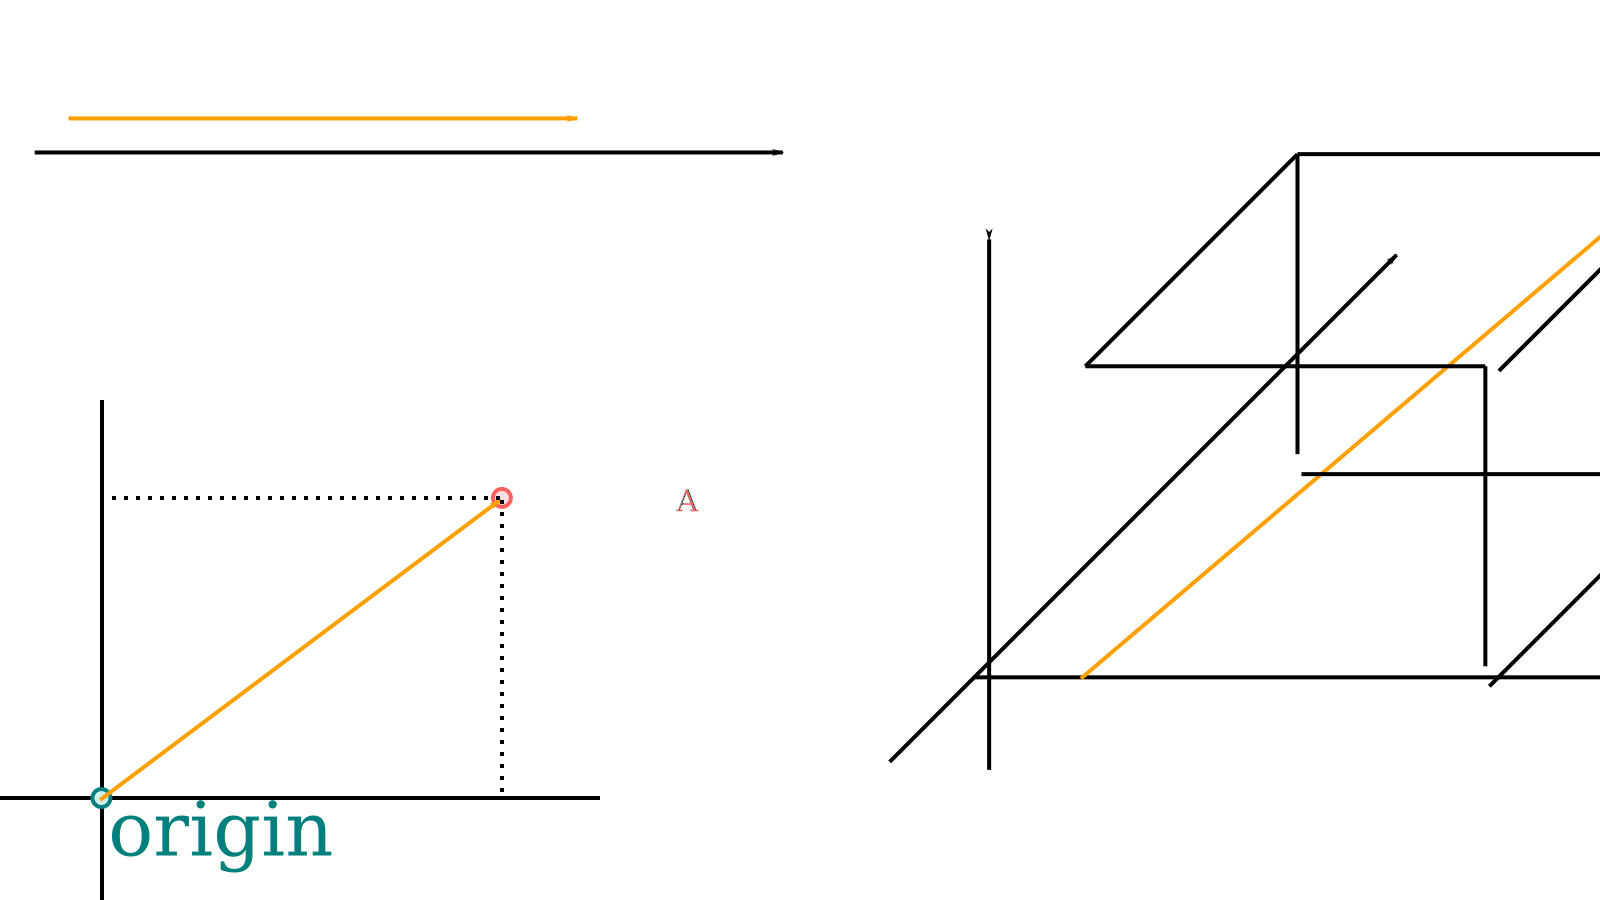
\includegraphics[width=1.0\linewidth]{figures/definePositionVector.png}}
	{\caption[Examples of Position Vector]{Three examples of position vectors shown as arrows in sand color pointed from the origin in teal color to the points in coral color: (a) $\bp_a$ in $\bR{1}$ at coordinate $(4)$ with length 4, (b) $\bp_b$ in $\bR{2}$ at coordinates $(4,\,4)$ with length $4\sqrt{2}$, (c) $\bp_c$ in $\bR{3}$ at coordinates $(4,\,4,\,4)$ with length $4\sqrt{3}$. The origins are located at $(0)$, $(0,\,0)$, and $(0,\,0,\,0)$ respectively.}\label{fig:definePositionVector}}
\end{figure}

%
%
\subsubsection{Subtracting Two Vectors}
\label{ch2sETBssLAsssS2V}
Among the various binary operators with which one could operate on vectors, this thesis is primarily concerned with subtraction, because it will be used to not only calculate the distance between each pair of adjacent points in the mesh, but also in order to interpolate and extrapolate the function values during the calculations of the \wmfv{s} described in detail in Sections~\ref{ch4sIE}~and~\ref{ch4sWM}.

In order to use the subtraction operator on two vectors in the same Euclidean space, one must simply subtract each component element-wise.~\cite{Weisstein19j} For example, given two points in $\bR{3}$, $A$ and $B$, the difference is calculated as
%
\begin{equation}
	A - B = (A_x - B_x,\,A_y - B_y,\,A_z - B_z)
	\label{eq:vectorSubtraction}
\end{equation}
%
which results in the single set of new coordinates, $\{C_x, C_y, C_z\}$, which both represents the point $C$ located there, or the position vector pointed there from the origin.

%
%
\subsubsection{L2-norm}
\label{ch2sETBssLAsssL2N}
The L2-norm may be seen elsewhere in the literature abbreviated as $L^2$ or $\ell^2$, or perhaps called the ``Euclidean norm'' or ``Euclidean distance''. It is so named because it is the ordinary, straight line distance between two points in Euclidean space, and in the case of a position vector $\bP$ in $\bR{3}$, those two points are the origin at $(0, 0, 0)$ and $\bp$ at the coordinates $\{\bP_x,\,\bP_y,\,\bP_y\}$~\cite{Weisstein19h}.

The purpose for calculating the L2-norm of a vector is to determine the ordinary, uni-dimensional length of the vector, regardless of the dimensionality of Euclidean space in which it is embedded. The significance of this distinction can be seen in Figure~\ref{fig:definePositionVector}; despite having all coordinates exclusively set to $4$, the position vector on (a) is of length $4$, in (b) it is of length $4\sqrt{2} \approx 5.657$, and in (c) it is of length $4\sqrt{3} \approx 6.928$.

To determine the length of a vector, one can use the equation for the L2-norm
\begin{equation}
	|\bp| \enspace=\enspace \|\bp\|_2 \enspace=\enspace \sqrt{x^2 + y^2 + z^2 + \ldots + n^2} \enspace:\enspace \bp \in \bR{n}
	\label{eq:l2norm}
\end{equation}

In this thesis, the L2-norm is denoted using the abbreviated symbols $|\bp|$. Please note the similar notation for the cardinality of a set $|\bP|$. While the matching symbols do represent somewhat similar concepts, cardinality is the count of elements in the set, but the L2-norm of a vector is calculated as in Equation~\ref{eq:l2norm}.~\cite[p.~26]{Mara12}
\todoReword{should I just use the long version?}

%
%
%
%
\subsection{Geometry}
\label{ch2sETBssG}
As vast and encompassing is geometry as a field of study, in this section, we will only introduce the few concepts which are of paramount importance for \fors{t}, including: geodesic discs for ensuring a consistent filter widow size for the duration of each convolution in Section~\ref{ch4sSEL}, the characteristics of a circle sector to be used in calculating the area and center of gravity in Section~\ref{ch4sACG}, as well as interpolation and extrapolation for calculating the \wmfv{s} in Section~\ref{ch4sWM}.
\todoResearch{weighted averaging using density}
\todoResearch{static filter window size importance}

%
%
\subsubsection{Geodesic Discs}
\label{ch2sETBssGsssGD}
Geodesy, the term from which geodesic discs get their name, is defined differently in many fields.\todoCitation{geodesy} A geodesic, defined in the original sense, was the shortest route between two points on the Earth's surface; so a straight line distance in curved space. In this thesis, we use the term geodesic disc to mean the surface area on a manifold, encompassed by a circle with a given radius, which itself is also embedded in $\bR{3}$, and reference to such a disc with the symbol $\bO$.
\todoResearch{create figure of geodeisc disc in 3d}

The significance being the similar mathematical treatment of all adjacent faces in any given neighborhood, in order to ensure a consistent filter window size for the duration of each convolution of \fors{t}, despite that given the nature of acquired \tdd{} as discussed in Section~\ref{ch2s3ssAVS3}, which likely all exist on different planes in $\bR{3}$. Also, from the geodesic disc, we derive the circle sectors which are described in detail in the next section.
\todoResearch{static filter window size importance}
\nomenclature[aa]{$\bO$}{a geodesic disc}%
\nomenclature[ab]{$\bO_v$}{a specific geodesic disc centered about the point $\bp_v$}%

%
%
\subsubsection{Circle Sectors}
\label{ch2sETBssGsssCS}
A circular sector, or circle sector, is the portion of a disc enclosed by two radii and an arc. In general, the larger area is known as the major sector, however \fors{t} is only concerned with the area of the other, smaller area, known as the minor sector as it is a natural way to partition a geodesic disc embedded in $\bR{3}$, where each sector can be delineated by the border of two triangular faces which likely exists on different planes.\todoReference{figure of geodesic disc in 3d, once made} Going forward, the minor circle sector will be abbreviated as just ``the circle sector'', or even more simply, ``the sector'', and will be denoted as $\bs$, or $\bs_i$ in reference to a specific circle sector, as described in Section~\ref{ch4sSEL}.%
\nomenclature[ba]{``the sector''}{or the circle sector; the minor sector of a circle defined by its radius and central angle}%
\nomenclature[bb]{$\bs$}{a circle sector}%
\nomenclature[bc]{$\bs_i$}{a specific circle sector}%

As the sector can be described entirely by the central angle $\alpha$ and the circle's radius\footnote{$\ell_{a,b}$ was chosen to represent the radius instead of the much more common $r$, because in \tdd{}, edges are not stored, yet distances between points can be calculated as shown in Section~\ref{ch2s3ssEL}} $\ell_{a,b}$, the area of the sector can be given as
%
\begin{equation}
	A = \pi \ell_{a,b}^2\frac{\alpha}{2\pi} = \frac{\ell_{a,b}^2\alpha}{2}
	\label{eq:areaOfCircleSector}
\end{equation}
%
because of the fact that in radians, the ratio of a sector's central angle $\alpha$ to the complete angle of the circle $2\pi$, is equal to the ratio of that sector's area to area of the whole circle.~\cite{Weisstein19d}%
\nomenclature[bd]{$A$}{an area of a circular sector}%

%
%
\subsubsection{Center of Gravity}
\label{ch2sEBTssGsssCG}
Along with area, the other important characteristic of a circle sector for \fors{t} is the centroid, or center of gravity, which is used in both Algorithms~\ref{alg:serialConvolveFilter}~and~\ref{alg:parallelConvolveFilter} in order to calculate the \wmfv{s}, by serving as the location to which the function values are interpolated, the operation which is discussed in the next section.

The center of gravity is named so, because it is the point where the sector would balance on a pin\footnote{given that it had been bestowed a volume with uniform density}. The center of gravity $\bc$ is calculated as the distance from the center point $\bp_a$, along the line which bisects the central angle $\alpha$, and is given by
%
\begin{equation}
	\check{\ell} := \frac{4\:\gelm\:\sin(\frac{\alpha_i}{2})}{3\,\alpha_i}
	\label{eq:ch2distToCoG}
\end{equation}%%
\nomenclature[ca]{$\bc$}{the center of gravity of circle sector $\bs_i$}%
\nomenclature[cb]{$\check{\ell}$}{the distance from $\bp_0$ to $\bc$}%

In the Figure~\ref{fig:circleSector}, a circle sector is produced by the points $\bp_a$, $\bp_b$, and $\bp_c$, has the central angle $\alpha$, which is bisected by a dotted line, and $\ell_{a,b}$ representing the length between points $\bp_a$ and $\bp_b$, which is equal radius of the circle. Also shown, is the center of gravity $\bc$, as well as $\check{\ell}$, the distance to $\bc$ from the center point $\bp_a$.

\begin{figure}[ht]
\ffigbox
	{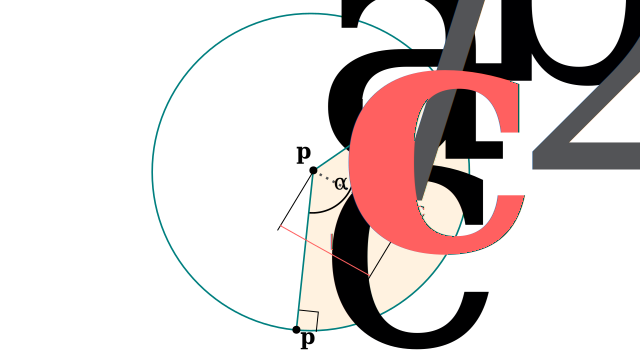
\includegraphics[width=0.6\linewidth]{figures/circleSector.png}}
	{\caption[A Circle Sector in Detail]{The circle sector produced by points $\bp_a$, $\bp_b$, and $\bp_c$, with $\alpha$ as the central angle bisected by a dotted line, and $\ell_{a,b}$ as the length between points $\bp_a$ and $\bp_b$ which is equal radius of the circle. Also labeled is the center of gravity $\bc$ as well as the distance from the center point $\bp_a$ to $\bc$, drawn in a coral color as $\check{\ell}$}\label{fig:circleSector}}
\end{figure}

The line which bisects the central angle of a circle sector, while not used explicitly in calculations, is an important concept for much of the computations used by \fors{t}, as will be seen in Chapter~\ref{ch4}. Therefore, we make a special note here that the abbreviated, ``bisecting line'', indeed refers to this line which splits the circle sector, and its central angle $\alpha$, into two equivalent halves.%
\nomenclature[cc]{``bisecting line''}{the line which bisects the central angle of a circle sector}%

%
%
\subsubsection{Interpolation \& Extrapolation}
\label{ch2sETBssGsssIE}
Simply stated, interpolation is a method of constructing new data points within the range of a discrete set of known data points, such as those points found in the discrete manifolds of in \tdd{}. There exist a large variety of methods for interpolating different kinds of data\todoCitation{different kinds of interpolation}, but in this thesis, we will only consider linear interpolation, which is simple to calculate\footnote{however can become imprecise in relation to the square of the distance between the data points.}\todoCitation{footnote:error of linear interpolation} and can be extended for n-dimensions\todoCitation{n-dimensional linear interpolation}.

Given the two data points in $\bR{2}$, $(x_a, y_a)$ and $(x_b, y_b)$, the $y_c$ coordinate of a third point located along a straight line drawn between the first two points, while also having the coordinate $x_c$, can be calculated as
%
\begin{equation}
	y_c = y_a + (y_b - y_a) \frac{x_c - x_a}{x_b - x_a}
	\label{eq:interpolationGeneral}
\end{equation}

To elaborate the concept of interpolation, now consider the two points $(1, 2)$ and $(5, 1)$, then find the $y$ coordinate of a point between them, located at the intersection of the line which contains the first two points and $x = 3$
%
\begin{align}
	y_c & = 2 + (1 - 2) \frac{3 - 1}{5 - 1} \\
	& = 2 + -1 \frac{2}{4} \enspace = \enspace  1.5
	\label{eq:interpolationSpecific}
\end{align}
%
We therefore interpolate the value halfway between the two given points to be $(3,\,1.5)$, which is halfway between as expected, as illustrated in Figure~\ref{fig:interpolation}.

Conversely, extrapolation is a method for constructing new data points \textit{outside} the range of a discrete set of known data points. The process of linear extrapolation is equivalent\footnote{The difference between interpolation and extrapolation is largely an academic one, owing primarily to the lack of boundaries and increasing error rates associated with extrapolation.} to linear interpolation; namely, first calculating the line between two points, then the $y$ coordinate of a third point at a new value of $x$, either greater than or less than both of the first two points.

As illustrated by Figure~\ref{fig:interpolation}, the similarities and differences between the processes of interpolation and extrapolation, become even more intuitive when seen graphically, where having chosen the two points $\bp_a$ and $\bp_b$, a third point $\bp_c$ is interpolated between the two points, while the fourth point $\bp_d$ is extrapolated outside their domain.

\begin{figure}[ht]
\ffigbox
	{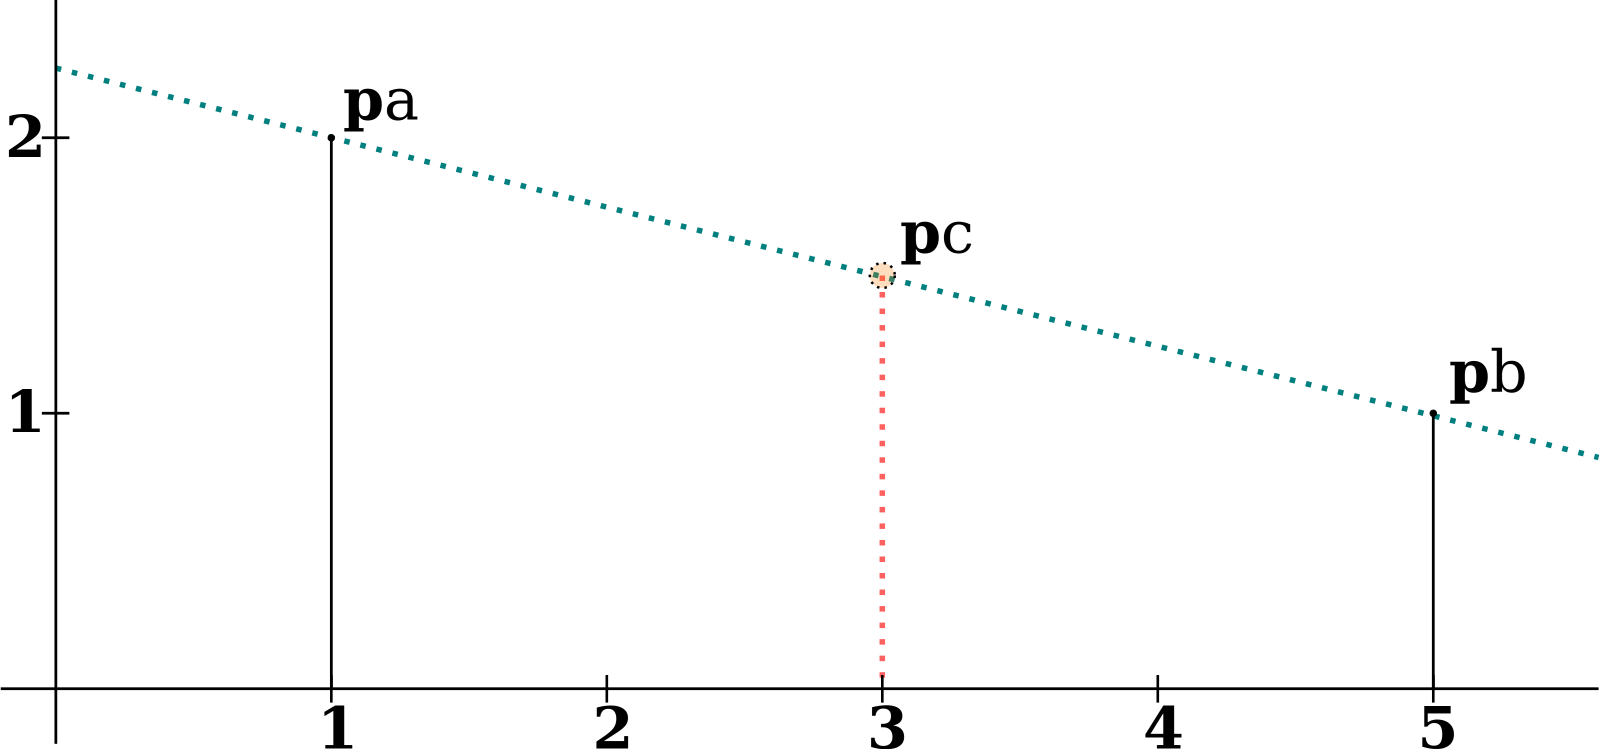
\includegraphics[width=1.0\linewidth]{figures/interpolation.png}}
	{\caption[Interpolation between two points in $\bR{2}$]{$\bp_c$ is interpolated as a value between $\bp_a$ and $\bp_b$}\label{fig:interpolation}}
\end{figure}

Later in this thesis, we will use both interpolation and extrapolation together, in order to calculate the \wmfv{s} at the center of gravity of circle sectors, so that the function values may be weighted fairly in regards to their distance to the other points in the one-ring neighborhood, as discussed in detail in Section~\ref{ch4sIE}.

%
%
%
%
\subsection{Topology}
\label{ch2sETBssT}
Topology is the mathematical study of the properties of space that are preserved through deformations, twistings, and stretchings of objects\footnote{but not tearing or gluing}, which developed as a field of study from geometry and set theory through analysis of concepts such as space, dimension, and transformation. For example, a circle is topologically equivalent to an ellipse, because it can be deformed by stretching.~\cite{Weisstein19c}

Of all the major concepts studied in topology, this thesis is only concerned manifolds, as \tdd{} is composed primarily of two-dimensional discrete manifolds embedded in three-dimensional space, as well as neighborhoods, the general concept from which one-ring neighborhoods are derived, thus the basis upon which \fors{t} is founded.

%
%
\subsubsection{Manifolds}
\label{ch2sETBssTsssM}
A manifold is a topological space that is locally, but possibly not globally, Euclidean; a concept that is central to many parts of geometry because it allows complicated structures, such as the triangle mesh, to be described and understood in terms of the simpler, local topological properties. Said another way, this means that a manifold is an $n$D-subset of an Euclidean space $\mathbb{R}^{>n}$.~\cite[p.~199]{Mara12} For example, 1-dimensional manifolds in $\mathbb{R}^{2}$ include lines and circles, and 2-dimensional manifolds in $\mathbb{R}^{3}$, also called surfaces, can include commonly-known shapes such as the plane, the sphere, and the torus, but also of prime importance for this thesis, the triangle mesh.

The significance to our research, is that each convolution of \Fors{t} is comprised of calculations of the \wmfv{s} at the central point of a one-ring neighborhood, having weighted the function values in relation to the distance between each neighbor, and because those distances are uniformly dissimilar in acquired \tdd{}\todoCitation{tdd{} is not regular}, maintaining a consistent filter window size is only accomplished by defining the geodesic disc, which exists on the manifold defined by the mesh. Therefore, as discussed in more detail in Chapter~\ref{ch4}, the weights may be calculated sector-wise, as if all sectors were on the same plane, greatly reducing the complexity of the entire procedure.

%
%
\subsubsection{Neighborhoods}
\label{ch2sETBssTsssN}
A neighborhood is also one of the basic concepts of topology. Intuitively speaking, a neighborhood of a point is a set of points containing that point, where one can move in any direction without leaving the set. While determining the neighborhood is trivial for uni-dimensional manifolds\footnote{where each neighborhood only consists of a point, and the two points to either side of it on the line}, and relatively simple for regular two-dimensional manifolds\footnote{such as with a 2D-image, whose pixels have at most four neighbors in orthogonal directions with a geometric distance of 1, as well as four neighbors at the diagonal directions with a geometric distance of $\sqrt{2}$}, determining the neighborhood becomes more complicated for irregular surfaces like those found in \tdd{}. With those surfaces, one must determine the set of neighbors using the associations that define the triangular faces; the details of which are covered in detail in Section:~\ref{ch2s3ssORN}, after the necessary topics regarding \tdd{} have already been discussed.

Figure~\ref{fig:neighborhoods} illustrates the differences among one-ring neighborhoods in different kinds of manifolds: (a) a regular square mesh as with pixels of a digital image, (b) a regular triangle mesh, as in a hexagonal tessellation, then in (c) the figure shows two very different neighborhoods in a single, irregular triangle mesh typical of acquired \tdd{}. In particular, notice in (c) the completely arbitrary shape and size of the one-ring neighborhoods found in the irregular triangle mesh; even the number of neighbors varies widely. From this observation is where much of the motivation behind \fors{t} came.

\begin{figure}[ht]
\ffigbox
	{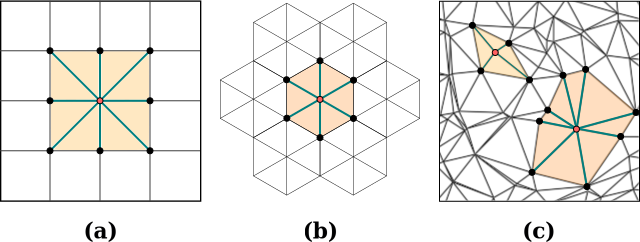
\includegraphics[width=1.0\linewidth]{figures/neighborhoods.png}}
	{\caption[One-ring neighborhoods in regular and irregular meshes]{One-ring neighborhoods in (a) a regular square mesh, as in pixels of a digital image (b) a regular triangle mesh, as in a hexagonal tessellation (c) an irregular triangle mesh, typical of acquired \tdd{}}\label{fig:neighborhoods}}
\end{figure}

%
%
%
%
%
%
\section{\tdd}
\label{ch2s3}
The data upon which one convolves \fors{t} is called \tdd\todoCitation{\tdd{} name origin, BB82 from Mara12}. As described in Section~\ref{ch2s3ssM}, \tdd{} consists primarily of a single mesh $\bM$, which is composed of $\bP$, a set of points, and the set $\bT$, consisting of triangular faces, each to be covered in Sections~\ref{ch2s3ssP} and~\ref{ch2s3ssF} respectively. \tdd{} also comes in two distinct flavors depending on its origin: acquired or synthetic, as discussed in Section~\ref{ch2s3ssAVS3}. The data can also include a texture map and other various types of information stored as scalar or vector fields, as elaborated on in~\ref{ch2s3ssFV}.

%
%
%
%
\subsection{Points}
\label{ch2s3ssP}
A point $\bp$ is the most primitive element of \tdd{}. ``Point'' is the abbreviated form of ``measuring point'', and is also known in other fields of study as a vertex, or a position vector $\bR{3}$\todoCitation{other names for a point}. A point is defined by the 3-dimensional Cartesian coordinates $x$, $y$, and $z$, and in \tdd{}, points are generally unique and not required to be in any particular order. In this thesis, a point is addressed using several different subscripts, depending on the context.

In this thesis, when referring to a point in $\bP$, $v$ is used as the globally unique index; the index with which we can define the set
%
\begin{equation}
	\bP := \left \{\:\bp_v \mid v \in \mathbb{N}, \;\text{and}\; 1\leq v \leq v_{max}\:\right \}
	\label{eq:defineSetOfPoints}
\end{equation}
%
where $v_{max}$ is the maximum index\footnote{\label{indicesFootnote}Beginning indices with 1 is significant because of the discordant conventions between addressing the first element of a data structure with 0 in programming languages, such as C++ and python, versus addressing first elements with 1, as is the standard for mathematical literature. Because this thesis should indeed be considered mathematical literature, we will always start indices at 1, and only use index 0 for special cases. For example, $\bp_0$ is used in Chapter~\ref{ch4} to represent the center point of the one-ring neighborhood.} of points in the data, and is equivalent to the cardinality of the set of points $|\bP|$.%
\nomenclature[ea]{$\bP$}{the set of points $\bp$ in $\bM$}%
\nomenclature[eb]{$\bp_v$}{a specific point in $\bP$}%

Otherwise, when referencing to a point within a particular face or neighborhood, the three corners can be referenced indirectly\footnote{or even more generally, as $\bp_a$, $\bp_b$, and $\bp_c$ in the case of Equation~\ref{eq:defineEdgeLengthFace}, or in the case of a nested loops: as $\bp_j$ and $\bp_{\sjpo}$ in Algorithms~\ref{alg:serialConvolveFilter}~and~\ref{alg:parallelConvolveFilter}} as $\bp_i$, $\bp_{\sipo}$, and $\bp_{\sipt}$, or directly as $\bp_0$\footref{indicesFootnote}, $\bp_1$, $\bp_2$, etcetera.~\cite[p.~25]{Mara12}%
\nomenclature[ec]{$\bp_i$}{also $\bp_{\sipo}$, and $\bp_{\sipt}$; one of three indirectly referenced points comprising a face}%

%
%
%
%
\subsection{Faces}
\label{ch2s3ssF}
Faces are the another primitive element of \tdd{}. As we are working exclusively with triangular meshes~\cite[p.~26]{Mara12}, we define a face $\bt$ by the set of three distinct points, which we will index in clockwise order\footnote{It is worth mentioning here that many software packages, such as the GigaMesh Framework~\cite[p.~89]{Mara12}, may expect counter-clockwise ordering of indexes. This is significant because the ordering provides an orientation by which visualization software can apply texture and/or lighting. The only mathematical significance of the ordering is the sign of the area of a face, and totally inconsequential when the absolute value is expected, as shown by~\cite[p.~2]{Braden86}. This is yet another example of the difference between the conventions of mathematical literature versus those of computer science. And again, because this thesis should indeed be considered mathematical literature, we will continue to follow the conventions of mathematical literature.}~\cite[p.~4]{Mara17}.
\todoResearch{does the "right-hand-rule apply here?"}
%
\begin{equation}
	\bt := \left \{\,\bp_a,\,\bp_b,\,\bp_c\right \} = \left \{\,\bp_1,\,\bp_2,\,\bp_3\right \}
	\label{eq:defineFaces}
\end{equation}

With the introduction of faces comes the concept of adjacency. A face $\bt_i$ is said to be adjacent to another face $\bt_j$ if, and only if, they share together the same subset of two points. Similarly, a point $\bp_a$ is said to be adjacent to another point $\bp_b$ if, and only if, the set $\{\bp_a, \bp_b\}$ is a subset of at least one face $\bt \in \bT$. A synonym for adjacent is ``neighboring'', and this thesis will use both interchangeably. \todoReword{add equation for these identities}\todoReword{index entry for adjacent}

Figure~\ref{fig:triangularFaces} shows two adjacent triangular faces $\bt_1$ and $\bt_2$, and the relationship between their points $\bp_a$, $\bp_b$, and $\bp_c$, their edge lengths $\ell_a$, $\ell_b$, and $\ell_c$, and their clockwise orientation. Because the concept illustrated in this figure is fundamental to understanding the structure of all \tdd{}, therefore also \Fors{t}, and yet may not be immediately intuitive without proper context, we reference this figure several times throughout the rest of this thesis.

\begin{figure}[ht]
\ffigbox
	{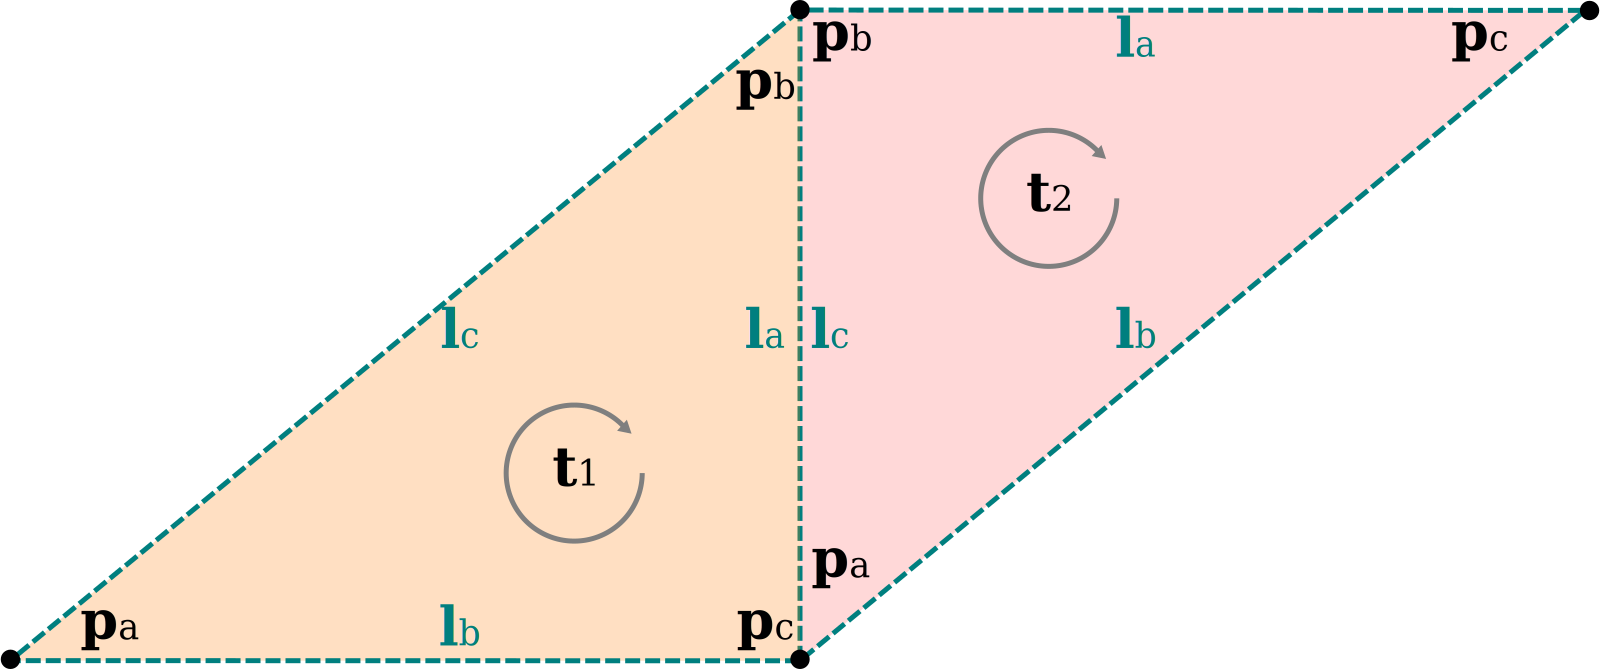
\includegraphics[width=1.0\linewidth]{figures/triangularFaces.png}}
	{\caption[Two Triangular Faces]{Two adjacent triangular faces $\bt_1$ and $\bt_2$, showing the relationship between their points $\bp_a$, $\bp_b$, and $\bp_c$, their edge lengths $\ell_a$, $\ell_b$, and $\ell_c$, and their clockwise orientation.}\label{fig:triangularFaces}}
\end{figure}

Each distinct triangular face is addressed using the global index $k$, and when taken together, comprise the set
%
\begin{equation}
	\bT := \left \{\:\bt_k \mid k \in \mathbb{N}, \;\text{and}\; 1\leq k \leq k_{max}\:\right \}
	\label{eq:defineSetOfFaces}
\end{equation}
%
where $k_{max}$ is the maximum index of faces in the data, and is equivalent to the cardinality of the set of faces $|\bT|$.%
\nomenclature[fa]{$\bT$}{the set of faces $\bt$ in $\bM$}%
\nomenclature[fb]{$\bt_k$}{a specific face in $\bT$}%

%
%
%
%
\subsection{Edge Lengths}
\label{ch2s3ssEL}
As illustrated in Figure~\ref{fig:triangularFaces}, each triangular face is implicitly composed of three edges. Despite the fact that an edge is not typically\footnote{Other data structures, such as the Winged-Edge~\cite[p.~1]{Baumgart75}, may use edges as a primitive element} a primitive element of \tdd{}, we will endeavor to define the length of an edge $\ell$, because edge lengths are of particular significance for both the design and implementation of \fors{t}.

What is also particularly interesting about Figure~\ref{fig:triangularFaces}, is that when edge lengths are defined by the points of specific faces, each non-border edge length, illustrated in the figure as $\ell_a$ in $\bt_1$, and $\ell_c$ in $\bt_2$, will be labeled twice, despite representing the same distance.

When in the context of a particular face $\bt_k$, we will use a single index to define the length
%
\begin{equation}
	\ell_a := |\bp_b - \bp_c| \enspace:\enspace \left \{\,\bp_a,\,\bp_b,\,\bp_c\right \} = \bt_k
	\label{eq:defineEdgeLengthFace}
\end{equation}%
\nomenclature[ga]{$\ell_i$}{the length of the edge opposite the point $\bp_i$ of a specific face}%
%
and double indices when an edge length is referenced in relation to a specific point $\bp_v$ and its neighbor $\bp_i$
%
\begin{equation}
	\ell_{\sv{i}} := |\bp_i - \bp_v|
	\label{eq:defineEdgeLengthPoint}
\end{equation}%
\nomenclature[gb]{$\ell_{\sv{i}}$}{the length of the edge between points $\bp_v$ and $\bp_i$}%

Please note the similar notation for the cardinality of a set $|\bP|$, to that for the calculation for the length of the edge $|\bp_i - \bp_v|$ as defined in Equation~\ref{eq:defineEdgeLengthPoint}. While cardinality is simply the count of elements in the set, the length is calculated as the L2-norm of the referenced vector.~\cite[p.~26]{Mara12}

\begin{equation}
\begin{aligned}
	|\bp_i - \bp_v| & = \lVert\bp_i - \bp_v\rVert_2 \\
					& = \sqrt{(x_i-x_v)^2 + (y_i-y_v)^2 + (y_i-y_v)^2}
	\label{eq:defineEdgeLengthCalc}
\end{aligned}
\end{equation}
\todoResearch{can I avoid sqrt altogether by performing entire algorithm squared?}

%
%
%
%
\subsection{Meshes}
\label{ch2s3ssM}
In \tdd{}, a mesh $\bM$ is the digital representation of a discrete manifold embedded in $\bR{3}$, and is typically\footnote{except in the case of specifically designed synthetic data~\ref{ch7sSD}} two-dimensional, non-planar and comprised of non-regular, triangular faces composed of connected points.~\cite[p.~25]{Mara12} A mesh is the set defined as
%
\begin{equation}
	\bM := \left \{\bP,\:\bT\right \}
	\label{eq:defineMesh}
\end{equation}%
\nomenclature[da]{$\bM$}{a mesh; the set including the sets of all points $\bp$ and faces $\bt$}%
%
with the set $\bP$ consisting of points, and the set $\bT$ consisting of triangular faces.

Many 3D-scanners produce point clouds\todoCitation{3D-scanners produce point clouds}, which as the name suggests, are comprised soley of a set of points $\bP$ and do not provide the set $\bT$. However, it is possible, and necessary for the production of a mesh, to perform a point set triangulation\todoCitation{perform a point set triangulation} in order to connect $\bP$ into a set of triangle faces, enabling one to combine the two sets into a mesh.~\cite[p.~26]{Mara12} For example, during our experiments, we perform the well-known Delaunay triangulation\todoCitation{Delaunay triangulation} in order to produce a mesh from a randomly generated point cloud\todoReference{experiments}.
\todoResearch{add figure of point cloud to triangulation}

%
%
%
%
\subsection{One-Ring Neighborhoods}
\label{ch2s3ssORN}
It was mentioned in Section~\ref{ch2sETBssTsssN}, that it is a non-trivial task to determine the neighborhood of a point $\bp_v$, which exists in an irregular triangle mesh embedded in three-dimensions. Having now examined the definitions of points, faces, and meshes, we can now formalize the one-ring neighborhood in \tdd{} as
%
\begin{equation}
	\bN_v := \left \{\;\bp_i\;:\;\left \{\,\bp_i,\,\bp_v\right \} \subseteq \bt \quad \forall \bt \in \bT\;\right \}
	\label{eq:defineNeighborhood}
\end{equation}%
\nomenclature[ha]{$\bN_v$}{the set of points comprising the one-ring neighborhood about $\bP_v$}%
\nomenclature[hb]{$\bp_i$}{a one-ring neighbor of $\bp_v$}%
%
which in words, means that the neighborhood $\bN_v$ is defined as the set of points $\bp_i$ such that both $\bp_i$ and $\bp_v$ are two points of a triangular face $\bt$, for all faces in the mesh. Therefore, the adjacency of points is defined by the co-membership within a face $\bt$, from the set of faces $\bT$.

When taken together, all the neighborhoods $\bN_v$ comprise a set of sets of neighbors; the family of sets
%
\begin{equation}
	\bN := \left \{\bN_v,\,\bN_{v+1},\ldots,\,\bN_{v_max}\right \}
	\label{eq:defineNeighborhood}
\end{equation}%
\nomenclature[hc]{$\bN$}{a family of sets of neighbors, the set of neighborhoods}%
This definition shares the indices $v$ and $v_{max}$ with the definition for a set of points, Equation~\ref{eq:defineSetOfPoints}, to highlight the fact that neighborhoods are defined per point, therefore there must be a correlation in the cardinality between the two sets.

Conversely, the cardinality of each individual neighborhood $|\bN_v|$ will likely vary among other neighborhoods in $\bN$, however, the value must always be $\geq 2$, and though there is no upper limit, $|\bN_v|$ is typically $\leq 12$. Furthermore, the neighboring points are always indexed in a clockwise direction for the same reasons as discussed in Section~\ref{ch2s3ssF}.
\todoResearch{get real upper limit for n}.%

As illustrated in Figure~\ref{fig:neighborhoods}, the set of black points are the neighbors $\bp_i$ which belong to $\bN_v$, what is known as a one-ring neighborhood\footnotemark of $\bp_v$, because they are directly connected with the center point $\bp_v$ drawn in coral color. The moniker originates from graph theory where each adjacent point is said to have a relative distance of 1 within the graph of the mesh. \footnotetext{The one-ring can be extended to a 2-ring by taking the union of the neighborhood $\bN_v$ with the neighborhood of each one-ring neighbor $\bp_i$, which adds to the neighborhood, points with the relative distance of 2 within the graph. This iterative concept can be repeated k times and the neighborhood is than referred to as k-ring. Unfortunately, regardless of the fact that the relative distance within the graph can not be assumed equal to the geometric distance nor geodesic distance, it is still used throughout the literature – especially in the field of Computer Graphics.~\cite[p.~29]{Mara12}}
\todoBackground{add a subsection on graph theory in basic theory section}

Our solution for maintaining a constant filter window size while convolving \fors{t} over neighborhoods of varying shapes and sizes is to determine the global minimum edge length, then use that as the radius of the geodesic disc centered at the central point of a neighborhood, in order calculate the \wmfv{s} of each circle sector, after interpolating each value function value from the neighboring points to the center of gravity, as explained in greater detail in Chapter~\ref{ch4}, later in this thesis.

%
%
%
%
\subsection{Acquired vs Synthetic \tdd{}}
\label{ch2s3ssAVS3}
The corpus of all \tdd{} exists in two flavors, acquired and synthetic data, with each being handily classifiable by the fashion in which it was generated, and the characteristics innate to those techniques.\todoReword{consider adding a figure here showing difference, or referencing a figure or pair of figures that does}

Acquired \tdd{} is typically captured as a point cloud utilizing various methods, such as: LiDAR (Light Detection and Ranging), Structured Light, or Structure from Motion~\cite[p.~19]{Mara12}. Then the data is exported from software packages accompanying the 3D-scanners as either just the point cloud as a simple set of points $\bP$, or optionally as a triangle mesh $\bM$, described by one or more scalar-fields. Acquired \tdd{} also often consists upwards of a million points and as many as twice that number of faces\todoReference{the interesting experimental finding about face to vertex ratio; add as a footnote}. These exported meshes ~\cite[p.~25]{Mara12} uniformly contain noise and may exhibit other complexities for analysis, such as: non-manifold points, multiple borders and holes in the surface, inverted face orientation, non-manifold edges, and agglutination or degenerate faces. ~\cite[p.~28-32]{Mara12}

Conversely, synthetic \tdd{} is artfully crafted to avoid the complexities exhibited by acquired data. When modeling 3-dimensional objects, synthetic \tdd{} can require significantly less memory for storage, as simplifications can be made for large regular surfaces. For example, even the largest flat, rectangular surface can be modeled with only four points and two faces, whereas the acquired data methods require that the Nyquist–Shannon sampling theorem\todoCitation{Nyquist Shannon Theorem} be obeyed for the smallest detectable feature throughout the entire surface.~\cite[p.~19]{Mara12}~\cite[p.~3]{Mara17}

For our experiments\todoReference{experiments}, we created another kind of synthetic \tdd{} which does not model a 3D-object. Instead, these synthetic-mesh generators produce different types of tessellations on arbitrarily large, planar surfaces, accompanied by a configurable scalar-field of function values.

%
%
%
\subsection{Function Values}
\label{ch2s3ssFV}
In addition to the three Cartesian coordinates, point which comprise a mesh may also contain other relevant data in the form of scalar fields, or vector fields, when combined together into multi-dimensional data. This information, which is stored at each point $\bp$, often includes data regarding: RGB color, material type, reflectivity, transparency, quality, confidence, or the resulting function values from an analytical filter such as the Multi-Scale Integral Invariants (MSII) filter~\cite[p.~21]{Mara12}, but can be extended to include data important to other fields of study, such as: infrared or ultraviolet light, temperature, rainfall, population, crime-rates, etc; essentially, any kind of data that may be measured at a point. As \fors{t} will currently\todoReference{future work/applications} only process a single field at a time, we can define a scalar field simply as the set of function values
%
\begin{equation}
	\bF := \left \{\: f_v \mid v \in \mathbb{N}, \;\text{and}\; 1\leq v \leq v_{max} \:\right \}
	\label{eq:defineSetOfFunctionValues}
\end{equation}%
\nomenclature[ia]{$\bF$}{the set of function values $f$; a scalar field}%
\nomenclature[ib]{$f_v$}{a specific function value in $\bF$, corresponding to $\bp_v$}%
%
This definition shares the indices $v$ and $v_{max}$ with, Equation~\ref{eq:defineSetOfPoints}, the definition for a set of points, because indeed, it is a fact that the cardinality of $|\bF|$ must be equal to $|\bP|$
%
\begin{equation}
	|\bF| \mbeq |\bP|
\end{equation}
%
because function values are only stored alongside the Cartesian coordinates, 1-for-1 with points, due to \tdd{} existing as a discrete manifold. The significance of which is another motivating factor behind the research conducted in this thesis.

%
%
%
%
%
%
\section{Parallel Processing}
\label{ch2sPP}

%
%
%
%
\subsection{Architecture of Concurrency} %Hardware
Of the 4 classifications of the architectures of concurrency\todoCitation{Flynn, 1966 doi:10.1109/TC.1972.5009071.}, this thesis is primarily concerned with SIMD\footnote{or SIMT as is branded by NVIDIA}\todoCitation{NVIDIA SIMT 4.1. SIMT Architecture}, single instruction, multiple data streams, which is the architecture of commercial workstations in use today. The SIMD classification is characterized by single instructions being executed in parallel on multiple data, which means simultaneously, typically requiring synchronization before the results may be further processed.

Figure~\ref{fig:simdArchitecture}, illustrates a simplified impression of system which employs SIMD architecture.

\begin{figure}[ht]
\ffigbox
	{\includegraphics[width=1.0\linewidth]{figures/simdArchitecture.png}}
	{\caption[SIMD Architecture]{The architecture characterized as SIMD by Flynn's Taxonomy of systems, where a single instruction is executed simultaneously, in parallel, on }\label{fig:simdArchitecture}}
\end{figure}\todoCitation{Flynn, 1966 doi:10.1109/TC.1972.5009071.}

The major advantage obtained by implementing software in SIMD system is the speedup gained when repetitive tasks which would otherwise be executed serially in a loop, one after another, can instead be computed simultaneously, incurring only minor synchronization overhead. Any operation performed in linear algebra, such as the multiplication of an entire vector by a scalar, is thus made much more scalable in regards to the time required to complete the computation for growing sizes of vectors.

This concept can be extended to more complex programs, and indeed, the topic of the research presented in this thesis is implementing the convolutions of the complex algorithm for \Fors{t} to be executed for every point in a mesh, simultaneously, in parallel, on a SIMD system.

All modern computers implement some form of parallelism, be it multi-core or multi-threaded processors, stream processors as found in GPUs, or networks of supercomputers or data centers. This thesis will focus on implementing \fors{t} in a way which can utilize the parallelism provided by the array of stream processors found in a commercially available GPGPU.

GPGPU stands fo General Use Graphics Processing unit, as coined by Mark Harris, the founder of GPGPU.org\todoCitation{Mark Harris}, coined the term GPGPU.and it describes the hardware

The technology

%\subsection{Host Memory and Device Memory}
\todoBackground{memory vs speed}
Hardware consists of memory and processors. Memory is divided into a hierarchy which starting at the registers on the processors themselves, increases in capacity, but decreases in speed.\todoReword{moves away from} Of particular interest to this thesis...\todoReword{continue}



%
%
%
%
\subsection{Serial Computation \& Threads}
\todoBackground{"spawning a thread"}
In a very general sense, when a computer executes a serial program, it proceeds one instruction at a time, sequentially in the order that it is written, reading and writing to memory as required. Individually, these are called threads of execution, and a single processing core can only process a single such thread at a time, however, it can rapidly perform context switching\todoCitation{context switching} among a multitude of self-contained threads, each with their own unique ids and memory addresses, in order to give the illusion of parallel processing.

As memory to be processed by a thread is stored somewhere in a hierarchy which increases in size, but decreases in speed as one moves from the processor's registers, it is likely that a context switch will cause what is known as a cache miss\todoCitation{cache hit or miss, check Lang}, which incurs a time penalty while the processing stalls and the required memory is read from slower hardware sources.



%
%
%
%
\subsection{Program Correctness}
\ldots

%
%
\subsubsection{Control \& Data Dependencies}
\label{ch2sPPssCS}
%Data Dependencies: ~\cite[p.~358]{Lang17}
%Section~\ref{ch2sACssCVP}
%Data Partitioning:
%Calculations depend on specific data structures.~\cite[p.~357]{Lang17}
%As in edge lengths depend on the neighborhoods.
\todoResearch{https://en.wikipedia.org/wiki/Loop-level\_parallelism}
%True (Flow) Dependence	S1 ->T S2	A true dependence between S1 and S2 means that S1 writes to a location later read from by S2
%Anti Dependence	S1 ->A S2	An anti-dependence between S1 and S2 means that S1 reads from a location later written to by S2.
%Output Dependence	S1 ->O S2	An output dependence between S1 and S2 means that S1 and S2 write to the same location.
%Input Dependence	S1 ->I S2	An input dependence between S1 and S2 means that S1 and S2 read from the same location.
The concepts of control and data dependencies are not new ones, and can be dated back to the invention of multi-pass compilers\todoCitation{Data Dependencies and multi-pass compilers}. The field of study regarding the details is called dependence analysis and has far-reaching consequences from business management, economics, as well as software optimization\todoCitation{dependence analysis}. In general, the basic concept behind both control and data dependencies is that some procedure A is said to be dependent on another procedure B, if A requires B to be executed first.

Figure~\ref{fig:simpleControlDependency} shows the ubiquitous if-then control structure as a simple example of a control dependency. It reads, ``if B is true, then do A''. In this case A is control dependent on B, because B must execute before it can be determined wether or not to execute A.

\begin{figure}[ht]
	\includestandalone[width=0.35\textwidth]{figures/tikz/simpleControlDependency}
	{\caption[If-Then Control Dependency]{A simple example of control dependency using the if-then control structure, with each distinct operation colored in teal, and control dependency marked with an arrow.}\label{fig:simpleControlDependency}}
\end{figure}

Figure~\ref{fig:dataDependencyOfL2Norm} illustrates the less-than-simple example of data dependencies inherent to calculating the L2-norm of a position vector in $\mathbb{R}^{3}$, which has already been seen in Equation~\ref{eq:l2norm}, and will be seen often in this thesis. There are six individual procedures involved with calculating the L2-norm: three squarings, two additions, and one square root. The three squaring procedures are totally independent of each other and can be performed in any order, indeed even concurrently, in relation to one another. In contrast, the two additions are totally dependent on their addends. While the order in which the first two of the three addends are used is inconsequential, the first addition is always dependent on the completion of two squarings, and the second addition is dependent on not only the sum from the first addition, but the product of the third squaring as well. Finally, because the square root procedure is dependent on the execution of both additions, it also inherits their dependencies on the squaring procedures, and therefore must wait until the very end before executing last.\todoResearch{name of this inheritance, associative?}

\begin{figure}[ht]
	\includestandalone[width=1.0\textwidth]{figures/tikz/dataDependencyOfL2Norm}
	{\caption[Data Dependencies in the L2-norm Calculation]{The data dependencies inherent to calculation of the L2-norm of a position vector in $\bR{3}$, with each distinct operation colored in teal, and data dependencies marked with arrows. The centered block in sand color represents an exclusive-or situation, abbreviated as xor, where one, and only one pair of operations shall execute.}\label{fig:dataDependencyOfL2Norm}}
\end{figure}

%
%
\subsubsection{Critical Sections}

%
%
\subsubsection{Mutexes}
%Mutexes and semaphores (binary semaphore}
While it is true that any locking mechanism can be expensive to both compute time and memory, \todoResearch{how expensive are locking mechanisms} typically, with acquired \tdd{}, the ratio of points in $\bP$ to the average neighborhood size \todoReword{add symbol for average neighborhood size} approaches $|\bP|$, therefore the speedup gained by exploiting the concurrency is definitely\todoResearch{quantify the cost} worth the cost of the added synchronization overhead when computing with even moderately sized meshes on a SIMP or SIMT modeled architecture.
starts at ~\cite[~p.20]{Lang17}

%
%
\subsubsection{Explicit Synchronization}%3.2.5.5.3. Explicit Synchronization}
\todoBackground{synchronizeThreads()}
sand color to highlight the fact that the values stored in memory will change throughout the life of the total procedure, and without the protection of a locking mechanism, therefore, extra care must be taken so that the implementation of the parallel variant of the serial algorithm will maintain correctness.

%
%
%
%
\subsection{Evaluation and Analysis of Concurrent Algorithms}~\cite[p.~330]{Lang17}
\subsubsection{Timing}
\begin{equation}
	N = input size (num. ops)
	P = processor count
	Ts(N) = Sequential execution time
	Tbest(N) = Optimal execution time
	TP(N, P) = Parallel runtime
\end{equation}
\subsubsection{Speedup, efficiency}
	Speedup:
S(N, P) = Tbest(N)/TP(N, P)

	Efficiency:
E(N, P) = Tbest (N)/PTP(N, P) = S/P

	Costs:
C(N, P) = PTP(N, P)

\subsubsection{Degree of Parallelism}
	0 < q < 1 is the sequential part
	1-q = is the parallelizable part


%\subsection{Hardware Implementation}%4. Hardware Implementation}
%\section{CUDA extended C++: An interface for GPGPU implementation}
%\subsection{CUDA C Runtime}%3.2. CUDA C Runtime}
%\subsection{Versioning and Compatibility}%3.3. Versioning and Compatibility}
%\subsection{Versions <9, vs >= 9}
%
%\subsection{Iso-efficiency}
%	WK(P) = iso-efficient if it fulfills:
%	TO(WK(P), P) = KWK(P)~\cite[p.~350]{Lang17}
%
%\subsection{Scalability}
%	A parallel system is called scalable only if in has an iso-efficency function
%
%
%
%
%
\section{Summary}
%

\chapter{Related Work}
%
\section{2D filters}
%	like from Digital Image Processing: i.e. Jaehne~\cite[p.~00]{todoCitation}\todoCitation{}



\section{Work with Diffusion Processes}
%	like from Digital Image Processing: i.e. Jaehne~\cite[p.~00]{todoCitation}\todoCitation{}



\section{Other Mesh filters}
%	which I could have done~\cite[p.~00]{todoCitation}\todoCitation{}



\section{Other approaches to accelerate}
%	operations on a mesh~\cite[p.~00]{todoCitation}\todoCitation{}



\section{Summary}
%

%
\chapter{Fast One-Ring Smoothing}
\label{ch4}
In this chapter we present an updated version of \Forf{t}, based on the filter initially proposed by H. Mara and S. Krömker at the EUROGRAPHICS Workshop on Graphics and Cultural Heritage (2017) ~\cite[s.~3.2]{Mara17}. Since publication, further research has been conducted by the authors, and it was determined that improving the weighting methods was possible, therefore, modifcations to the algorithm were implemented directly within the GigaMesh \todoCitation{GigaMesh} framework. This chapter presents the as-yet-unpublished version of \forf{t} as it exists now, with more accuracte weighting based on the interpolation of function values to the center of gravity for each circular sector comprising the geodesic disc centered upon a vertex in a mesh.

%
%
%
%
\section{The Shortest Edge Length}
\label{ch4sSEL}
Given the triangle mesh of \tdd{} $\bM$, a superset of both a set of points $\bP$ and a set of faces $\bT$, the procedure for \forf{t}  begins by choosing a point $\bp_v$, which defines the one-ring neighborhood $\bN_v$, then calculating the shortest edge length $\elm$ among all the points $\bp_i$ adjacent to the center point $\bp_v$, which  is indexed locally within the neighborhood as $\bp_0$. That shortest edge length
%
\begin{equation}
	\elm(\bp_0) := \text{min}^{|\bN_v|}_{i=1}\,\big(|\bp_i - \bp_0|\big)
	\label{eq:localMinimumEdgeLength}
\end{equation}%
\nomenclature[ja]{$\bp_0$}{the center point of $\bN_v$}%
\nomenclature[jb]{$\elm(\bp_v)$}{the shortest edge length in $\bN_v$}%
%
when considered as a radius, defines the geodesic circle $\bO_v$ about the point $\bv$. Furthermore, to ensure that the filter window remains the same size for the entirity of the mesh\footnote{a footnote about filter window size importance}\todoReword{footnote about filter window size importance}\todoCitation{SBN-13: 9781598296204}\todoResearch{call to question the importance of global minimum edge length in light of the typo found in source}, we define
%
\begin{equation}
	\gelm := \min\left \{\elm(\bp_0) \;|\; \bp_0 \in \bM\,\right \}
	\label{eq:globalMinimumEdgeLength}
\end{equation}%
\nomenclature[jc]{$\gelm$}{the shortest edge length in $\bM$}%
%
as the shortest edge length among all adjacent points in the mesh $\bM$, so that in lieu of $\elm$, we can use $\gelm$ in all the following computations presented in this chapter.

Figure~\ref{fig:geodesicDisc} shows a typical configuration of a one-ring neighborhood with irregular faces, the geodesic disc $\bO$ with radius $\elm$, and the circular sectors $\bs_i$.

\begin{figure}[ht]
\ffigbox
	{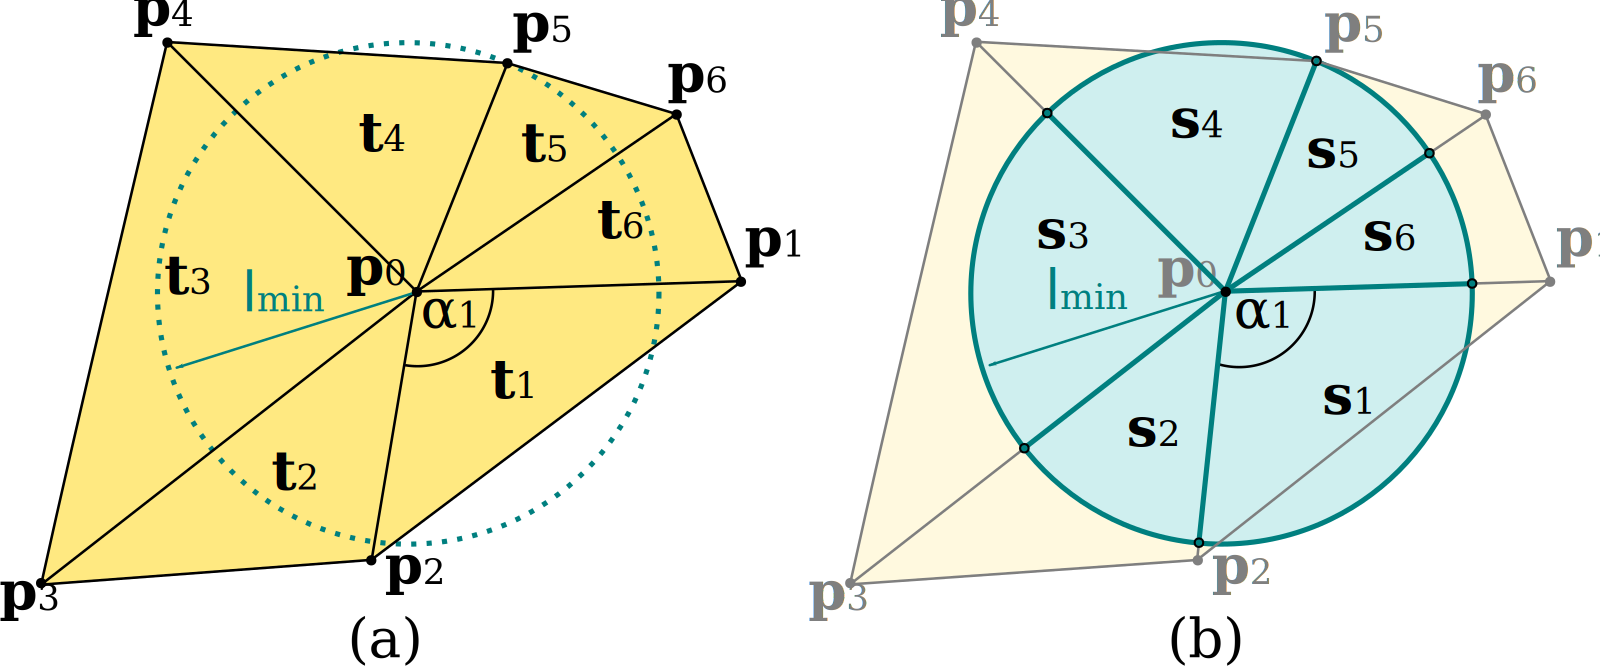
\includegraphics[width=1.0\linewidth]{figures/geodesicDisc.png}}
	{\caption[One-ring and geodesic disc]{A typical one-ring neighborhood $\bN$ with (a) irregular triangular faces $\bt_i$, the smallest edge length $\elm = \ell_5 = |\bp_5 - \bp_0|$ illustrated with a teal arrow as the radius of the geodesic disc, and $\alpha_1$ as the central angle of $\bt_1$ (b) the complete geodesic disc $\bO$, comprised of all its circular sectors $\bs_i$}\label{fig:geodesicDisc}}
\end{figure}%

%
%
%
%
\section{Angles}
\label{ch4sIA}
Before we can calculate the area of the circle sectors in $\bO_v$, we must first compute the inner angle $\alpha$ for each triangle $\bt$ in the neighborhood $\bN_v$. That is possible using the using the Law of Cosines~\cite{Weisstein19e}
%
\begin{equation}
	\alpha_i = cos^{-1}(\frac{|\bp_0 - \bp_{i}|^2 + |\bp_0 - \bp_{\sipo}|^2 - |\bp_i - \bp_{\sipo}|^2}{2\cdot|\bp_0 - \bp_{i}|\cdot|\bp_0 - \bp_{\sipo}|})
\end{equation}
%
or more compactly:
%
\begin{equation}
	\alpha = cos^{-1}\left (\frac{\ell_c^2 + \ell_b^2 - \ell_a^2}{2\cdot\ell_c\cdot\ell_b}\right )
	\label{eq:alphaFromEdgeLengths}
\end{equation}%
\nomenclature[ka]{$\alpha$}{the central angle of circle sector $\bs_i$}%

In order to interpolate the function values from each point over the entire sector, we must first interpolate the values one side of the bisecting line at a time, as will be discussed in detail in Section~\ref{ch4sWM}. For those coupled computations, the angles $\beta$ will be required, and having now obtained the $\alpha$, they can be calculated using a proxy right triangle and the third angle theorem\footnote{otherwise known as the Angle-Angle-Angle Theorem, abbreviated as AAA}~\cite{Weisstein19f} as
%
\begin{equation}
	\beta = \Big(\frac{\pi}{2} - \frac{\alpha}{2}\Big) = \frac{(\pi - \alpha)}{2}
	\label{eq:betaFromHalfAlpha}
\end{equation}%
\nomenclature[kb]{$\beta$}{the third angle with $\frac{\alpha}{2}$ and $\frac{\pi}{2}$}%

Figure~\ref{fig:anglesAndCenterOfGravity} extends Figure~\ref{fig:geodesicDisc} by enhancing the circle sector $\bs_1$ to show an example of the angles $\alpha/2$ and $\beta$, with the proxy right triangles used to calculate it, as well as the center of gravity which is discussed in detail in Section~\ref{ch4sIACG}.

%
%
%
%
\section{Area \& Center of Gravity}
\label{ch4sIACG}
Because a circle sector may be described entirely by its radius and central angle~\cite{Weisstein19d}, having now calculated $\gelm$ and $\alpha$, the area of the sector can be obtained using the formula
%
\begin{equation}
	A = \frac{(\gelm)^2\alpha}{2}
	\label{eq:circularSectorArea}
\end{equation}
%
and similarly $\check{\ell}$, the distance from the center point $\bp_0$ along the bisecting line to the center of gravity $\bc$ can be calculated directly using the formula
%
\begin{equation}
	\check{\ell} := \frac{4\:\gelm\:\sin(\frac{\alpha}{2})}{3\,\alpha}
	\label{eq:distToCoG}
\end{equation}%

Figure~\ref{fig:anglesAndCenterOfGravity} extends Figure~\ref{fig:geodesicDisc} by enhancing the circle sector $\bs_1$ to illustrate the center of gravity $\bc$ and its distance from the center point $\bp_0$. In general, while holding the radius constant, the smaller the angle $\alpha$ becomes, the longer the distance $\check{\ell}$ becomes.

\begin{figure}[ht]
\ffigbox
	{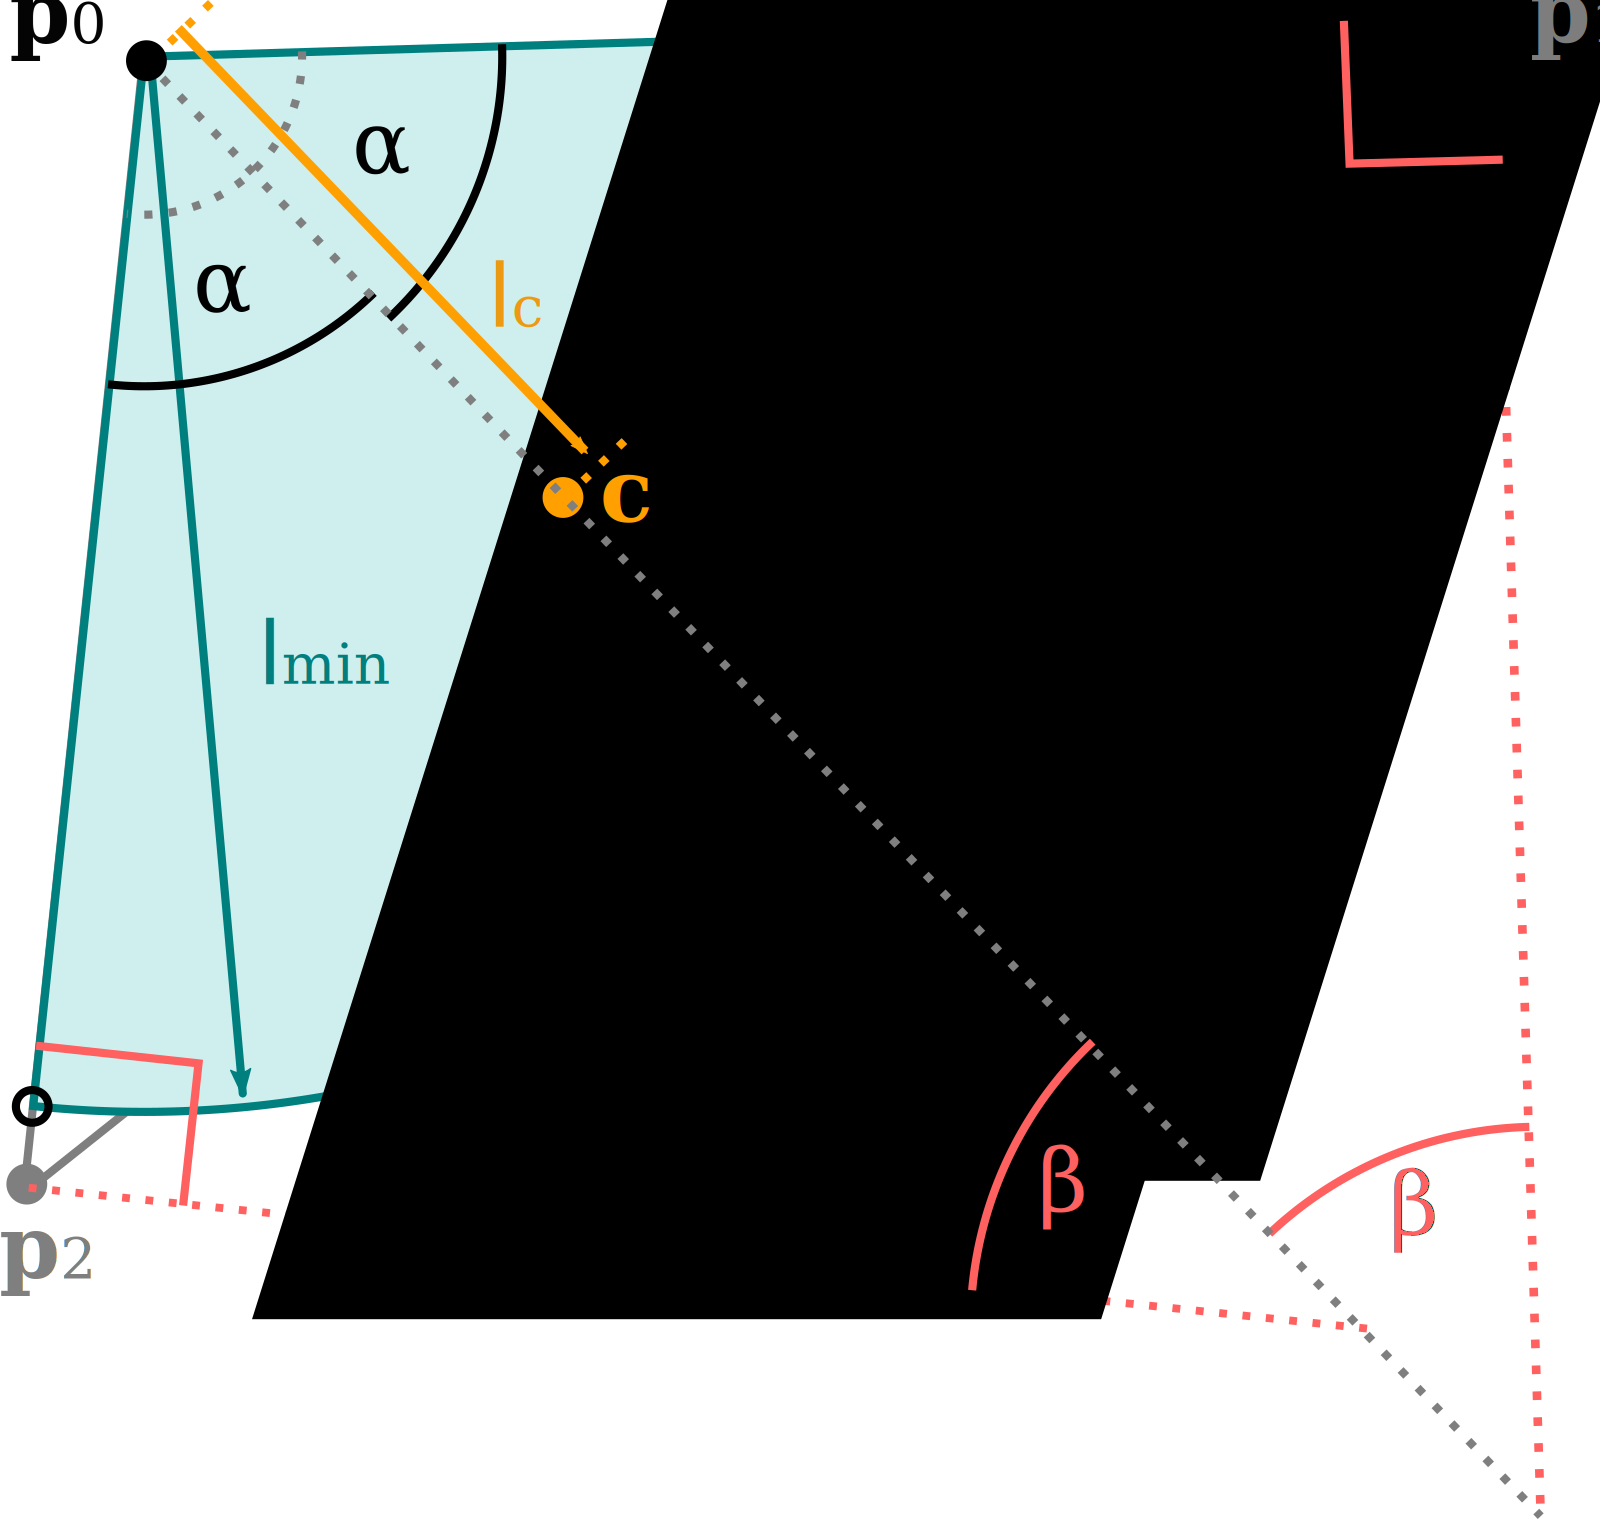
\includegraphics[width=0.8\linewidth]{figures/anglesAndCenterOfGravity.png}}
	{\caption[Angles and Center of Gravity]{An enhanced view of Figure~\ref{fig:geodesicDisc}, focusing on the circle sector $\bs_1$, showing $\alpha$ and the bisecting line in gray dots. In sand color is the center of gravity $\bc$ and $\check{\ell}$, the distance to it from $\bp_0$ along the bisecting line. Also shown in coral color, are the angles $\beta$, with the proxy right triangles used to calculate them.}\label{fig:anglesAndCenterOfGravity}}
\end{figure}%

%
%
%
%
\section{Interpolation}
\label{ch4sI}
Given the scalar field\footnote{\forf{T} is agnostic to the meaning of information represented by the data stored as function values in scalar fields, therefore, it can similarly convolve any such data. However, because the filter was designed to only convolve scalar fields, any multi-dimensional data, such as RGB color, must be processed individually as independent scalar fields.} of function values $\bF$, and having now calculated $\beta$, and $\gelm$, both values which are constant between halves of the circle sector, we can next use the Law of Sines~\cite{Weisstein19g} to obtain the constant ratio
%
\begin{equation}
	\zeta = \frac{\gelm}{\sin(\beta)}
	\label{eq:zeta}
\end{equation}%
\nomenclature[la]{$\zeta$}{constant ratio for interpolation derived from Law of Sines}%

It should be noted, that because the points $\bp_j$ and $\bp_{\sjpo}$ are likely\footnote{One need only to look at Figures~\ref{fig:geodesicDisc} or~\ref{fig:anglesAndCenterOfGravity} for an example of why that may be.} at different distances from the center point $\bp_0$, we must now begin calculating for each half of the circular sector individually. Therefore, while the index for $\zeta$ remains the match for the index of the circle sector $\bs$, we will now use the index $j$ to denote the side of the sector defined by its point $\bp_j$ or $\bp_{\sjpo}$.

Next, using $\zeta$, we can interpolate the offset from the original function values $f_j$ and $f_{\sjpo}$ at the points $\bp_j$ and $\bp_{\sjpo}$.
\begin{align}
	\tilde{\ell}_j & = \kern2pt\frac{\zeta}{\kern2pt\ell_j\kern2pt}\kern1pt = \kern3pt\frac{\zeta}{|\bp_j - \bp_0|}
	\label{eq:distanceIForInterpolation}\\
	\tilde{\ell}_{\sjpo} & = \frac{\zeta}{\ell_{\sjpo}} = \frac{\zeta}{|\bp_{\sjpo} - \bp_0|}
	\label{eq:distanceIp1ForInterpolation}
\end{align}%
\nomenclature[lb]{$\tilde{\ell}_j$}{also $\tilde{\ell}_{\sjpo}$, the distances for interpolation of $f_j$ and of $f_{\sjpo}$ towards $f_0$}%

Then, applying the offset distances $\tilde{\ell}_j$ and $\tilde{\ell}_{\sjpo}$, to the original function values $f_0$, $f_j$, and $f_{\sjpo}$, we can now interpolate the function values at $\bp_j$ and $\bp_{\sjpo}$ as
\begin{align}
	f'_j & = f_0(1 - \tilde{\ell}_j) + f_j\tilde{\ell}_j
	\label{eq:interpolatedFi} \\
	f'_{\sjpo} & = f_0(1 - \tilde{\ell}_{\sjpo}) + f_{\sjpo}\tilde{\ell}_{\sjpo}
	\label{eq:interpolatedFip1}
\end{align}%
\nomenclature[lc]{$f'_j$}{also $f'_{\sjpo}$, the interpolated values of $f_j$ and $f_{\sjpo}$ toward $f_0$}%

Figure~\ref{fig:interpolatedFunctionValues} illustrates an enhanced view of the circle sector $\bs_1$, continuing with the example introduced in Figure~\ref{fig:geodesicDisc}. It shows how, as a result of \tdd{} being composed of a discrete manifold, therefore, all function values must be stored 1-for-1 at the location of each point, instead of simply interpolating the function values at the corners of the geodesic disc, which are at the distance $\gelm$ between $\bp_0$ and $\bp_j$ or $\bp_{\sjpo}$, we must\todoAsk{but must we? we aren't ever going to save these values since they are unique to every neighborhood} instead interpolate as if $f_j$ were at $\gelm$, then calculate the $f'_j$ at the point $\bp_j$, so that either $f_0 \leq f_j \leq f'_j$ or $f_0 \geq f_j \geq f'_j$ are true\footnote{or both in the case that $\ell_j$ is equal to $\gelm$}, then likewise for $f'_{\sjpo}$. Furthermore, it illustrates how we must also interpolate from the points to the center of gravity, which we will discuss in detail Section~\ref{ch4sWM}.

\begin{figure}[ht]
\ffigbox
	{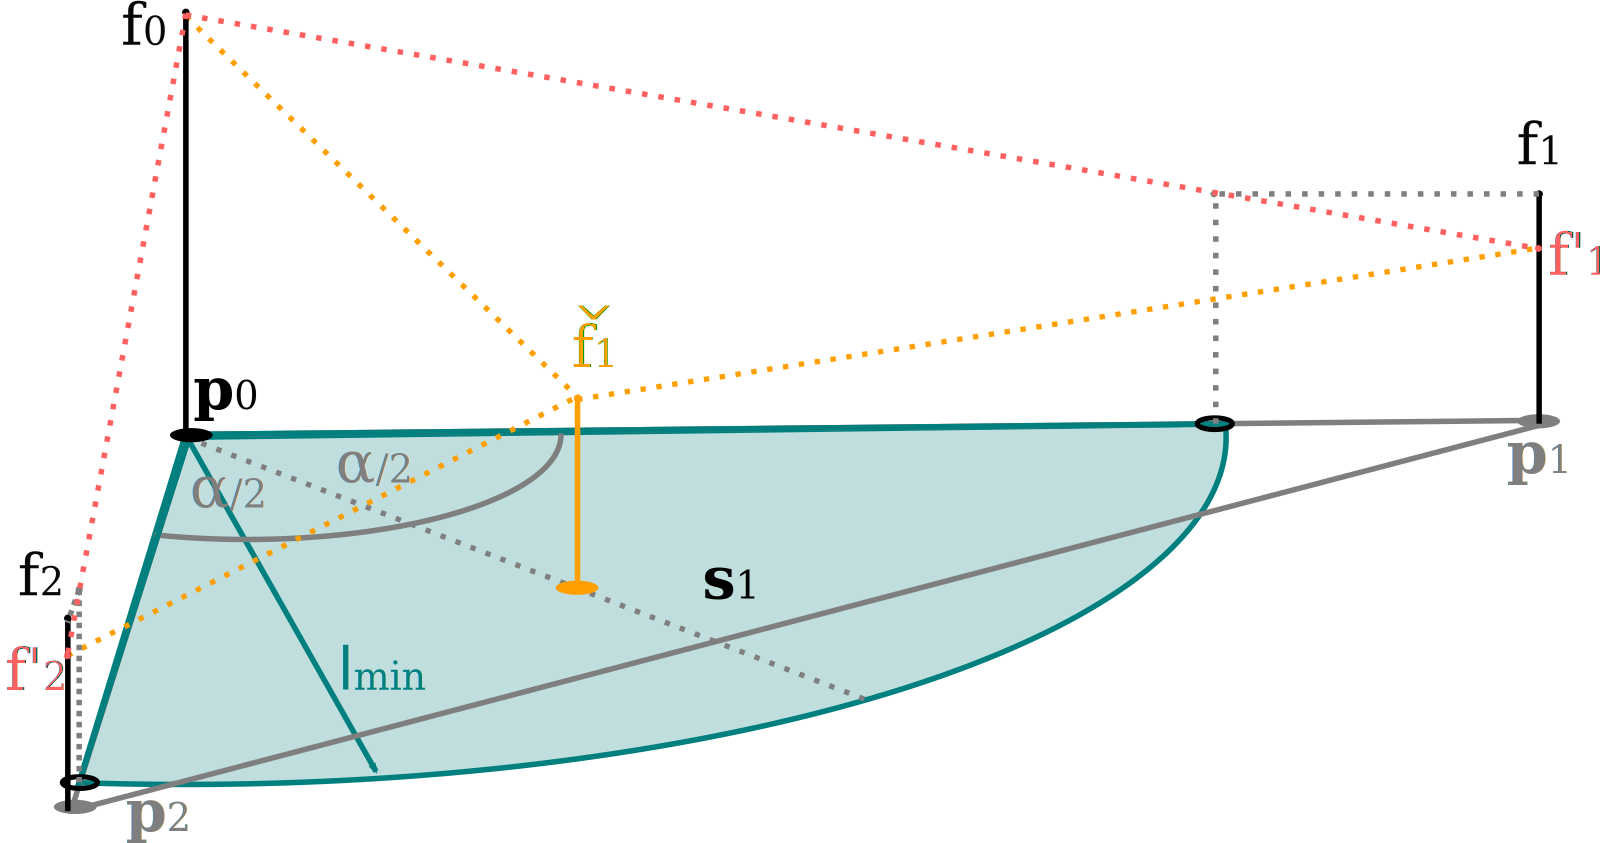
\includegraphics[width=1.0\linewidth]{figures/interpolatedFunctionValues}}
	{\caption[Interpolation of Function Values toward the Center of Gravity]{An enhanced view of the circle sector $\bs_1$, continuing with the example introduced in Figure~\ref{fig:geodesicDisc}, labeled in black are the function values $f_0$, $f_1$, and $f_2$, with the height of the line indicating magnitude of the value. Drawn in coral color, are the interpolated function values $f'_1$ and $f'_2$, along with the dotted lines illustrating how they were determined. In sand color is $\check{f}_1$, the weighted mean function value for the entire sector.}\label{fig:interpolatedFunctionValues}}
\end{figure}
\todoStyle{the fs need to match $f$}

%
%
%
%
\section{Weighted Mean}
\label{ch4sWM}
In order to calculate the weighted mean function value at the center of gravity $\bc$, of the circle sector $\bs_i$, we must combine the original function value at the center point $f_0$, and both interpolated function values, $f'_j$ and $f'_{\sjpo}$. Then using the distance to the center of gravity $\check{\ell}$, and the formula
\begin{equation}
	\check{f} = f_0\,(1 - \check{\ell}) + \frac{(f'_j + f'_{\sjpo})\,\check{\ell}}{2}
	\label{eq:weightedMeanAtCoGatSector}
\end{equation}%
\nomenclature[ma]{$\check{f}$}{the weighted mean function value at $\bc$ of $\bs_i$}%
we obtain the weighted mean function value $\check{f}$, at the center of gravity, representing the entire circle sector.

Figure~\ref{fig:interpolatedFunctionValues} illustrates $\check{f}$ in sand color as a volume over an enhanced view of the circle sector $\bs_1$, continuing with the example introduced in Figure~\ref{fig:geodesicDisc}. The figure also shows details pertaining to the interpolation of the function values $f_j$ and $f_{\sjpo}$, as discussed in detail in Section~\ref{ch4sFVI}.

Finally, we can compute the one-ring weighted mean function value at $\bp_0$ by first multiplying each interpolated function value located at each circle sector's center of gravity $\check{f}$, by each sector's area $A$, to obtain a volume of function value over the entire circle sector. Then by dividing the sum of all the function value volumes, by the total area of the geodesic disc $\bO_v$, we can compute
\begin{equation}
	f'_v := \frac{\sum A\check{f}}{\sum A} \quad \forall i \in \{1,\ldots,|\bt_v|\}
	\label{eq:meanFuncValAtPv}
\end{equation}%
\nomenclature[mb]{$f'_v$}{the one-ring weighted mean function value at $\bp_v$}%
the one-ring weighted mean\footnote{The one-ring smoothing filter can be modified to use the median operation, instead of the mean, by using all the equations except Equation~\ref{eq:meanFuncValAtP0} and then sorting the results of Equation~\ref{eq:weightedMeanAtCoGatSector}. The details of which can be found by the original publication ~\cite[s.~3.2]{Mara17}, but as it was not implemented in GPGPU for this thesis, we exclude the details here.} function value for $\bp_v$, which is the center point $\bp_0$ of the neighborhood $\bN_v$.

Figure~\ref{fig:weightedMean} illustrates the geodesic disc $\bO$, as introduced in Figure~\ref{fig:geodesicDisc}, with volumes of interpolated function value over each circle sector, which shall be divided by each sector's area in order to obtain the the one-ring weighted mean function value $f'_v$ at $\bp_v$.
\begin{figure}[ht]
\ffigbox
	{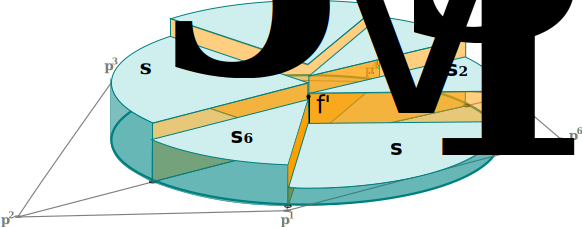
\includegraphics[width=1.0\linewidth]{figures/funcValVolumes.png}}
	{\caption[Weighted Mean Function Value $f'_v$at $\bp_v$]{The geodesic disc $\bO$, as introduced in Figure~\ref{fig:geodesicDisc}, with volumes of interpolated function values over each circle sector $\bs$, which shall be divided by each sector's area $A$ in order to obtain the the one-ring weighted mean function value $f'_v$ at $\bp_v$.}\label{fig:funcValVolumes}}
\end{figure}
%
\section{Summary}
\label{ch4sS}
In this chapter we presented an updated version of \Forf{t}, which since its original publication~\cite[s.~3.2]{Mara17}, now utilizes the entire area of the geodesic discs $\bO$ centered at each point in the mesh $\bp_v$, in order to calculate the weighted average of all the function values in its one-ring neighborhood. First, we illustrated in detail how one can calculate the globally shortest edge length $\gelm$, interior angles $\alpha$ and $\beta$, the area $A$, and the distance $\check{\ell}$ from the center point to the center of gravity $\bc$, for any given of a sector $\bs$ of a geodesic disc $\bO$ in a one-ring neighborhood $\bN$ of mesh $\bM$. Next, we provided the equations for interpolating the three function values $f_0$, $f_j$, and $f_{\sjpo}$, using the pairwise constant ratio $\zeta$, in order to obtain the weighted mean function value for each $\bs$, and finally the weighted mean function value $\bar{f_0}$ at point ${\bp_0}$ for the entire one-ring neighborhood $\bN$. Convolving this filter with the scalar field of function values at each vertex in a mesh, for any number of iterations, thus produces a smoothing effect with increasing intensity in relation to the number of iterations.

\chapter{Profiling \& Exploiting Concurrency}
In the previous chapter we presented an improved version of the Fast One-Ring smoothing filter for scalar fields on discrete meshes as it is currently implemented within the GigaMesh framework, and while it has improved accuracy, it is entirely serial in design so that unfortunately, its performance suffers greatly under the complexity of modern mesh sizes, which with the current high resolution scanners in use \todoCitation{hi rez scanners}... as large as \todoCitation{mesh sizes}. We will now endeavor to profile this as-yet-unpublished algorithm in order to discover opportunities to exploiting any cuncurrency and improve its performance.
\todoReword{is profile really the best word?}
%
\section{Serial Implementation}
\label{cFPECsSI}
In this section, with the goal of \sout{facilitating} understanding\todoReword{facilitating understanding sounds bad} of the implementation of the improved Fast One-Ring smoothing filter, we now combine all of the equations from the previous chapter,~\ref{eq:localMinimumEdgeLength} through~\ref{eq:meanFuncValAtP0} into an three-part algorithm using mathematical pseudo-code. \todoReword{better transition} The convolution of the filter requires that the one-ring neighborhoods be known and uses all edge lengths once per iteration, and twice for non-border edge lengths which are shared between adjacent neighborhoods. Thus, it is beneficial to split the algorithm into three distict parts, then save the results of the first two parts to be used in the iterative convolutions of the second part, all in order to increase efficency by reducing the number of calculations-per-iteration required.
\todoBackground{add adjacent neighborhoods to background}
\todoBackground{add convolution and convolve to background}
\todoBackground{mention how 3Ddata doens't save neighborhood information, and only winged pairs save edge info}
%
\subsection{Discover Neighborhoods}
Initially, one must discover all points $\bp_k \; \forall k \in \bN_v$ which are members of each neighborhood $\bN_v \; \forall v \in \bM$. Although building this family of sets outside of the principle loop adds an additional $2\cdot f^3$ operations, as we will see in Algorithm~\ref{alg:serialCompute}, doing so enables the main procedure to constrain the number of required iterations to only $\tau^{(v^k)}$, significantly decreased from the $\tau^{(v^{|\mathcal{F}|})}$ otherwise needed had the procedure been requried to discover $\bN_v$ in each iteration.
\todoBackground{family of sets, https://en.wikipedia.org /wiki/Family\_of\_sets}
%
\begin{algorithm}
	\DontPrintSemicolon
	\SetCommentSty{small}
	\SetKwFor{For}{for}{:}{}

	\SetKwInOut{Input}{Input}\SetKwInOut{Output}{Output}
	\Input{things for filter}
	\Output{new function values}

	\bigskip
	\FuncSty{serialBuildNeighborhoods}\FuncArgSty{(a,b)}\;
\nl	\For{$f \in \mathcal{F}$}{
\nl		\For{$i \in \{0,1,2\}$}{
			\linespread{1.5}\selectfont
%seperated
%\nl			$\bp_a \leftarrow \bp_{\big((i\kern-.7pt\scalebox{0.66}{+}\kern-1.2pt1)\%3\big)}$\;
%\nl			$\bp_b \leftarrow \bp_{\big((i\kern-.7pt\scalebox{0.66}{+}\kern-1.2pt2)\%3\big)}$\;
%\nl			$\bN_{\widehat{\bp_i}} \leftarrow \bN_{\widehat{\bp_i}} \cup \{\bp_a, \bp_b\}$\;
%together
\nl			$\bN_{\widehat{\bp_i}} \leftarrow \bN_{\widehat{\bp_i}} \cup \left \{\bp_{\big((\sipo)\%3\big)}, \bp_{\big((\sipt)\%3\big)}\right \}$\;\label{serialBuildNeighborhoodsComplexSubscripts}
		}
	}
	\caption{Serial algorithm for discovering the neighborhoods required by the Fast One-Ring smoothing filter, before it can begin iteratively convolving a mesh\label{alg:serialBuildNeighborhoods}}
\end{algorithm}%
\todoStyle{brackets are ugly}%
\nomenclature[fa]{$\mathcal{F}$}{the set of Faces comprising the mesh}%
\nomenclature[fb]{$\widehat{\bp_i}$}{the unique index for point $\bp_i$, correspondign to $v \in \bM$}%
\nomenclature[fc]{$\Ds$}{the most costly operation in the Fast One-Ring filter, due to use of $\sqrt{(\cdot)}$}%

Algorithm~\ref{alg:serialBuildNeighborhoods} uses complex subscripts in line~\ref{serialBuildNeighborhoodsComplexSubscripts}. The meaning is to increment over the set of points $\{\bp_0$, $\bp_1$, $\bp_2\}$, which define each face $\mathbf{f} \in \mathcal{F}$. The symbol $\widehat{\bp_i}$ represents the unique index for point $\bp_i$, corresponding to $v \in \bM$, so that we can discover the neighborhood $\bN_{\widehat{\bp_i}}$ by performing a union operation with the set of neighboring points $\left \{\bp_{\big((\sipo)\%3\big)}, \bp_{\big((\sipt)\%3\big)}\right \}$,\todoStyle{brackets are ugly} whose indices change incrementally with $i$ in order to always represent the two neighbors of $\bp_i \in f$.
\todoBackground{have defined $f$ already, and add to nomenclature, update entire document. deconflict with function symbol, should follow style of for faces $\mathbf{f}_i$, cardinality of should be $f$}
%
\subsection{Calculate Edge Lengths}
In Algorithm~\ref{alg:serialCalculateEdgeLengths}, we calculate the edge lengths $\eta_{vk} \; \forall v \in \bM, \; \forall  k \in \bN_v$, as well as the global minimum edge length $\gDm$ of $\bM$. Although building this set outside of the principle loop requires ${\Ds}^{(v^k)}$ operations, where $\Ds$ is the most costly operation in the entire algorithm\todoCitation{calculating $\Ds$ is expensive}, as we will see in Algorithm~\ref{alg:serialCompute}, doing so enables the main procedure to completly exclude all $\Ds$ operations from the principle loop, reducing the total count to only the initial $1\cdot v^k$, which is completely independant of $\tau$ and significantly decreased from the ${(2\,\xi_{border} + 4\,\xi_{non-border})\cdot\tau^v}$ otherwise needed had the procedure been required to calculate an edge length each time it was used in computation.
\todoReword{mention memory costs}%
\todoBackground{add $\Ds$}%
\begin{algorithm}
	\DontPrintSemicolon
	\SetCommentSty{small}
	\SetKwFor{For}{for}{:}{}

	\SetKwInOut{Input}{Input}\SetKwInOut{Output}{Output}
	\Input{things for filter}
	\Output{new function values}

	\bigskip
	\FuncSty{CalculateEdgeLengths}\FuncArgSty{(a,b)}\;
\nl	\For{$v\leftarrow 1\;\KwTo\;m$}{
\nl		\For{$k\leftarrow 1\;\KwTo\;n_v$}{
			\linespread{1.5}\selectfont
\nl			$\eta_{vk} \leftarrow |\bp_k - \bp_v|$\label{precal-bpkbpv}\tcc*[r]{every edge length}
\nl			$\gDm \leftarrow \min\{\gDm, \eta_{vk}\}$\tcc*[r]{Eq:~\ref{eq:globalMinimumEdgeLength}}
		}
	}
	\caption{Serial algorithm for the calculations required by the Fast One-Ring smoothing filter, before it can begin iteratively convolving a mesh\label{alg:serialCalculateEdgeLengths}}
\end{algorithm}%
\nomenclature[f03]{$v$}{the cardinality of $\bN$ about $\bp_i$}%
\nomenclature[f04]{$k$}{the index for a point in $\bN_v$}%
\nomenclature[f05]{$\eta_{vk}$}{the length of the edge between $\bp_v$ and $\bp_k$}%
% If alg.1 changes, update refence to number of new symbols.

Algorithm~\ref{alg:serialCalculateEdgeLengths} introduces five new symbols: $v$ is used to represent a unique index for each vertex in $\bM$; $k$ indexes each neighboring point in the one-ring neighborhood $\bN_v$; whose cardinality is $n_v$, $|\bp_k-\bp_v|$ from line~\ref{precal-bpkbpv} is analogous to $|\bp_i-\bp_0|$ from Equation~\ref{eq:localMinimumEdgeLength} when $\bp_v$ becomes $\bp_0$; and lastly, $\eta_{vk}$ is the length of the edge between $\bp_v$ and $\bp_k$.%
\todoReword{combine all $\xi \eta \delta$, all represent aan edge length}
%
\subsection{Computation}
In Algorithm~\ref{alg:serialCompute}, we illustrate the remaining steps required to process a mesh using the one-ring filter, after having completed the pre-calculations in~\ref{alg:serialCalculateEdgeLengths} and~\ref{alg:serialBuildNeighborhoods}.
\begin{algorithm}
	\DontPrintSemicolon
	\SetCommentSty{small}
	\SetKwFor{For}{for}{:}{}

	\SetKwInOut{Input}{Input}\SetKwInOut{Output}{Output}
	\Input{things for filter}
	\Output{new function values}

	\bigskip
	\linespread{1}\selectfont
	\FuncSty{Calculate}\FuncArgSty{(a,b)}\;
	\nl\For{$\tau\leftarrow 1\;\KwTo\;\#iterations$}{
	\nl	\For{$v\leftarrow 1\;\KwTo\;m$}{
	\nl		\For{$i \leftarrow 1\:\KwTo\:|\bN_v|$}{
				\linespread{2}\selectfont
	\nl			$\alpha_i \leftarrow$ \begin{large}
					$\text{cos}^{-1}\Big(\frac{
						(\eta_{\widehat{\bp_i},\widehat{\bp_{\sipt}}})^2 +
						(\eta_{\widehat{\bp_i},\widehat{\bp_{\sipo}}})^2 -
						(\eta_{\widehat{\bp_{\sipo}},\widehat{\bp_{\sipt}}})^2
					}{2
						(\eta_{\widehat{\bp_i},\widehat{\bp_{\sipt}}})
						(\eta_{\widehat{\bp_i},\widehat{\bp_{\sipo}}})
					}\Big)$\tcc*[r]{Eq:~\ref{eq:alphaFromEdgeLengths}}
				\end{large}
				\linespread{1.5}\selectfont
	\nl			$\beta_i \leftarrow (\pi - \alpha_i)\mathbin{/}2$\tcc*[r]{Eq:~\ref{eq:betaFromHalfAlpha}}
	\nl			\kern-2pt$A_i \leftarrow \gDm^2\alpha_i\mathbin{/}2$\tcc*[r]{Eq:~\ref{eq:circularSectorArea}}
	\nl			\kern-7pt$\Dc_i \leftarrow \big(2\:\gDm\:\sin(\alpha_i\mathbin{/}2)\big)\mathbin{/}(3\alpha_i\mathbin{/}2)$\tcc*[r]{Eq:~\ref{eq:distToCoG}}
	\nl			\kern1pt$\zeta_i \leftarrow \gDm\mathbin{/}\sin(\beta_i)$\tcc*[r]{Eq:~\ref{eq:zeta}}
	\nl			\For{$j \in {1,2}$}{
	\nl				\kern-8pt$\Dz_j \leftarrow \zeta_i\mathbin{/}|\bp_0 - \bp_j|$\tcc*[r]{Eq:~\ref{eq:distanceIForInterpolation},~\ref{eq:distanceIp1ForInterpolation}}
	\nl				$f'_j \leftarrow f_0(1 - \Dz_j) + f_j\Dz_j$\tcc*[r]{Eq:~\ref{eq:meanFuncValAtP0},~\ref{eq:interpolatedFip1}}
				}
	\nl			$f^\bs_i \leftarrow f_0(1 - \Dc_i) + \big((f_1 + f_2)\Dc_i\big)\mathbin{/}2$\tcc*[r]{Eq:~\ref{eq:weightedMeanAtCoGatSector}}
	\nl			\kern-2pt$\tilde{A}_v \leftarrow \tilde{A}_v + A_i$\tcc*[r]{Eq:~\ref{eq:meanFuncValAtP0}}
	\nl			$\tilde{f}_v \leftarrow \tilde{f}_v + A_if^{\bs}_i$\tcc*[r]{Eq:~\ref{eq:meanFuncValAtP0}}
			}

	\nl		$\bar{f}_v \leftarrow \tilde{f}_v\mathbin{/}\tilde{A}_v$\tcc*[r]{Eq:~\ref{eq:meanFuncValAtP0}}
		}
	}
	\caption{Serial algorithm for the Fast One-Ring smoothing filter for scalar fields on discrete manifolds\label{alg:serialCompute}}
\end{algorithm}%
\nomenclature[f06]{$\eta^v_{1,2}$}{the length of the edge between $\bp_i$ and its neighbors in $\bt_i$, $\bp_1$ and $\bp_2$}%
%
\section{Data Partitioning}~\cite[p.~357]{Lang17}
Data Partitioning is important.


%
\section[Acceleration by GPGPU]{Acceleration by GPGPU (General-purpose
computing on graphics processing units)}

%
\section{Summary}
then calculate all the edge lengths $\eta_{vk}$, as well as the global minimum edge length $\gDm$. Afterwards, one may efficiently convolve the filter, for as many number of iterations as required to achieve the desired smoothing effect.


\chapter{Meat 3}
\section{Summary}
Lorem ipsum dolor sit amet, consectetur adipiscing elit. Morbi tincidunt eget 
ipsum eu iaculis. Cras vel sem eu velit eleifend porta vel sit amet massa. Etiam 
a posuere nunc. Aenean aliquam viverra dapibus. Aliquam ac eros a purus feugiat 
rhoncus. Donec faucibus ut nibh ut cursus. Aliquam erat volutpat. Proin efficitur 
nulla sit amet iaculis condimentum. Cras placerat leo vitae venenatis feugiat. In 
hac habitasse platea dictumst. Orci varius natoque penatibus et magnis dis 
parturient montes, nascetur ridiculus mus. In aliquet sagittis dui eu pulvinar. 
Morbi a arcu eu dolor sagittis varius. Aliquam dignissim tortor sed tortor 
suscipit, eget imperdiet mauris convallis.

%
\chapter{Experiments \& Evaluation}
An important test for any filter\todoCitation{} \todoResearch{convolutions in furior space, think Jaehne}, is to apply the filter iteratively upon a Dirac delta function\todoCitation{}.
\section{Synthetic Data}
Synthetic Examples are generated with ideal vertices, unlike acquired examples.

\subsection{Random Noise Function}\todoResearch{Currently, no meshes exist for research}

\subsection{Vector Fields}\todoResearch{Set up: choose color with different RGB, like Cyan. Add noise to each channel. Use filter to process each channel seperately and display results.}

\subsection{A Flat surface with Dirac Delta function}
\subsubsection{Square Tesselation, two triangles}
\begin{figure}[ht]
\ffigbox
	{\begin{subfigure}[b]{0.48\linewidth}
		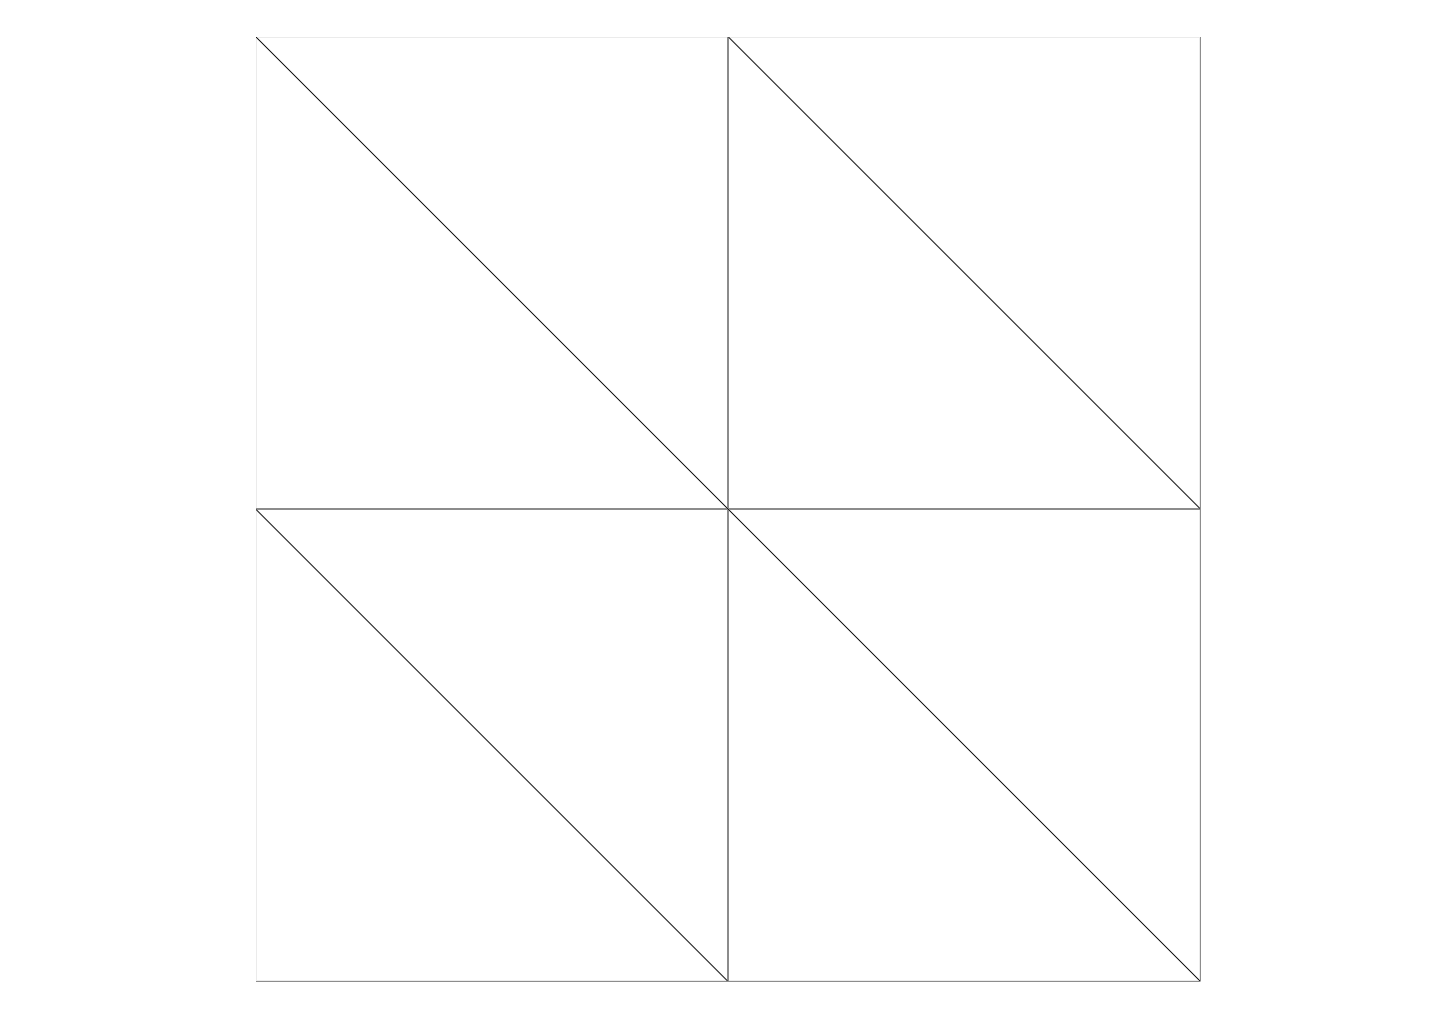
\includegraphics[width=1.0\linewidth,height=0.32\textheight,keepaspectratio]{data/synthetic_meshes/square_tesselation_2tri_Dirac_delta_1_v9_f8_wireframe.png}
		\caption{Sq2 v9\_f8 wireframe}\label{fig:sq2.a}
	\end{subfigure}
	\begin{subfigure}[b]{0.48\linewidth}
		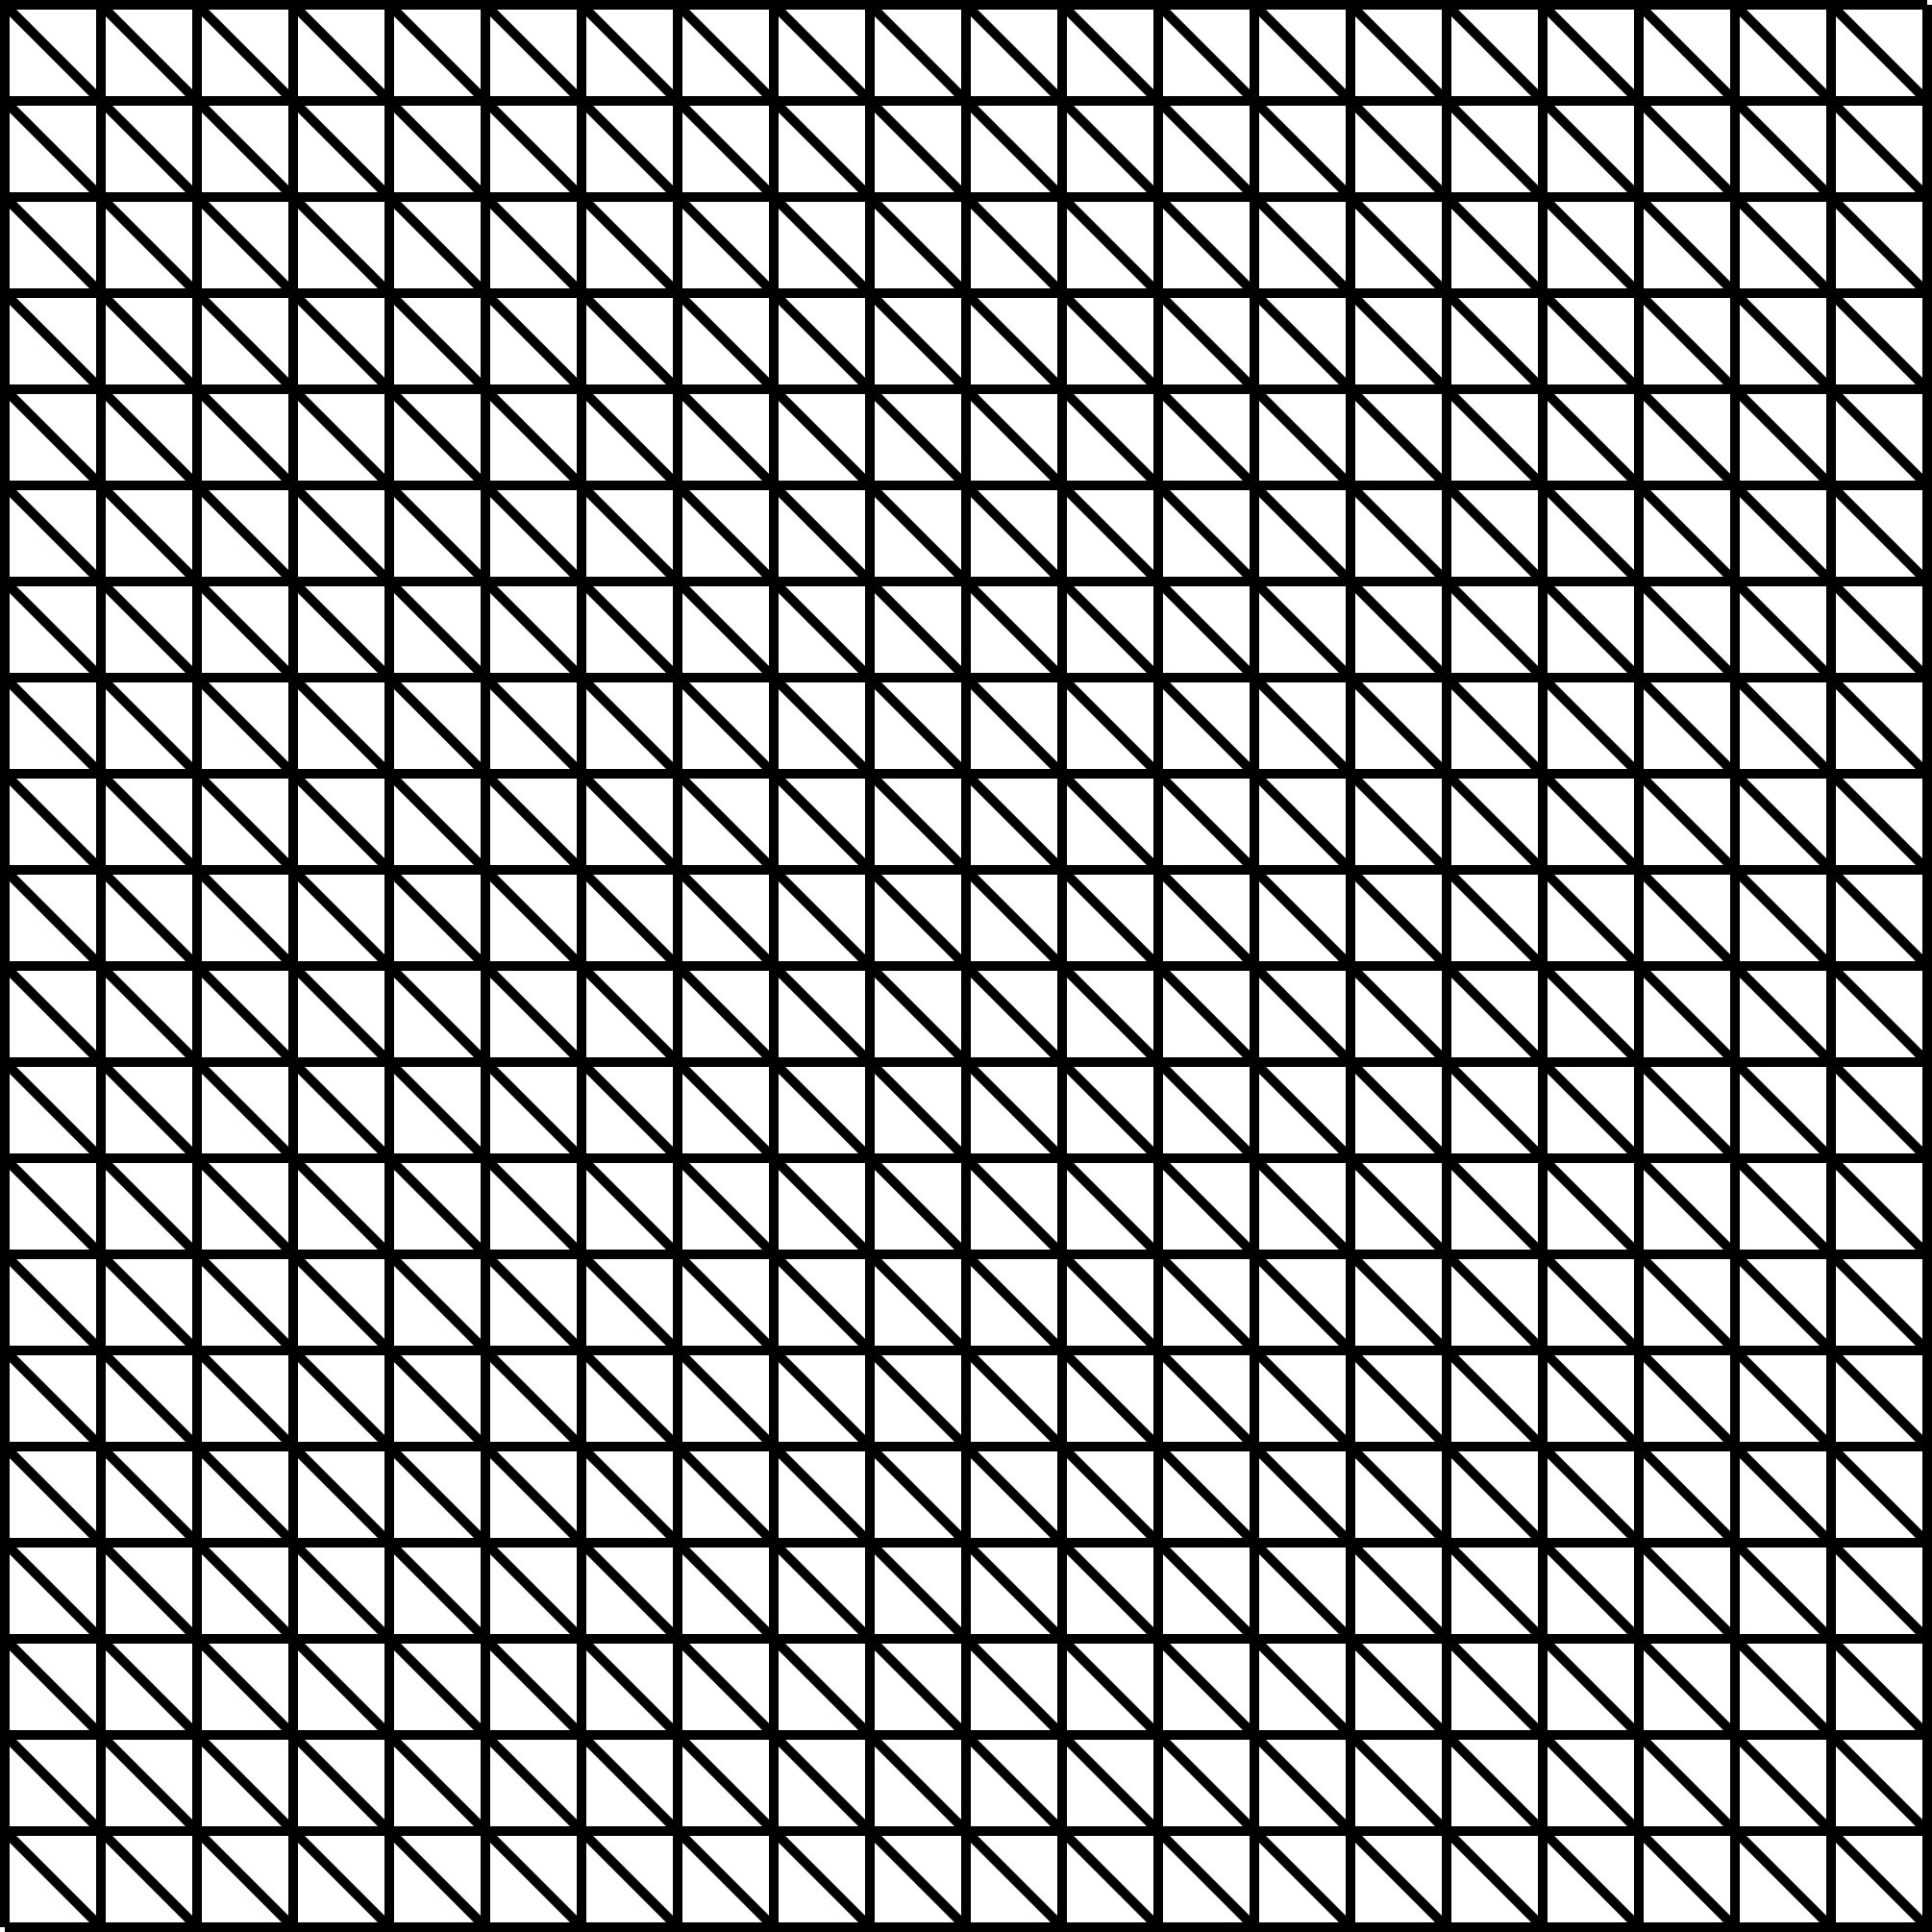
\includegraphics[width=1.0\linewidth,height=0.32\textheight,keepaspectratio]{data/synthetic_meshes/square_tesselation_2tri_Dirac_delta_10_v441_f800_wireframe.png}
		\caption{Sq2 v441\_f800 wireframe}\label{fig:sq2.b}
	\end{subfigure}

	\bigskip
	\begin{subfigure}[b]{0.48\linewidth}
		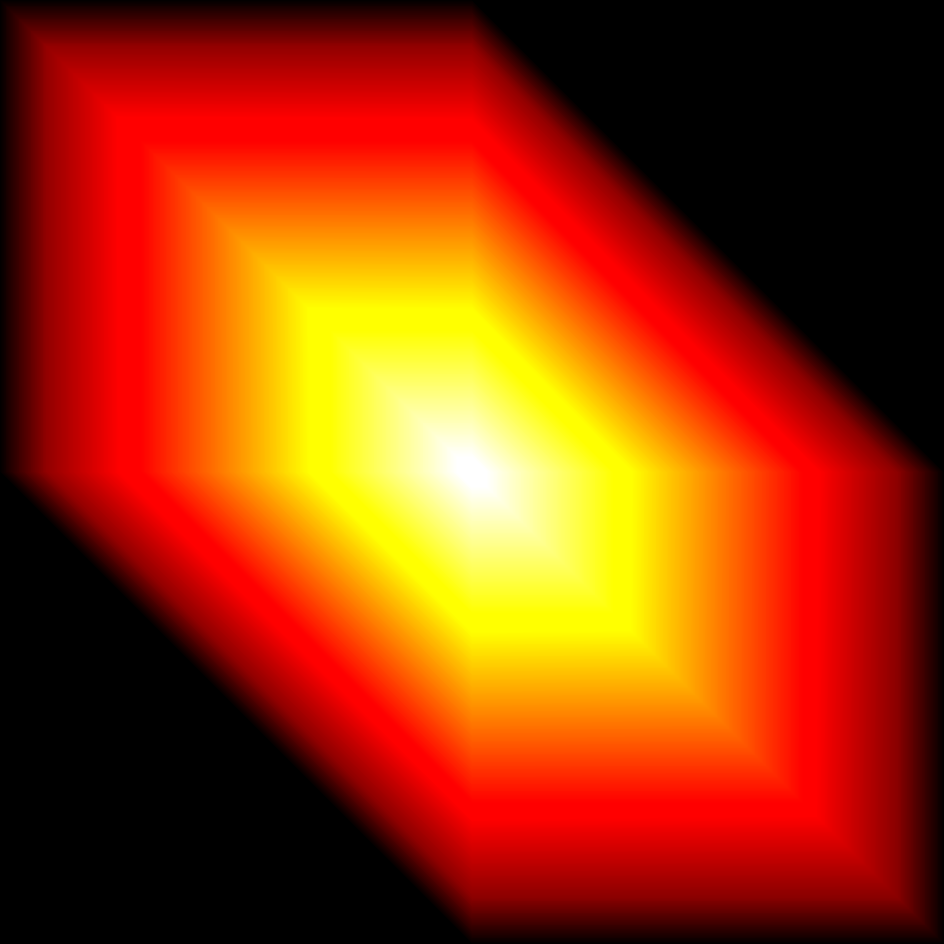
\includegraphics[width=1.0\linewidth,height=0.32\textheight,keepaspectratio]{data/synthetic_meshes/square_tesselation_2tri_Dirac_delta_1_v9_f8_funcvals_0iter_crop.png}
		\caption{Sq2 v9\_f8 iter 0}\label{fig:sq2.c}
	\end{subfigure}
	\begin{subfigure}[b]{0.48\linewidth}
		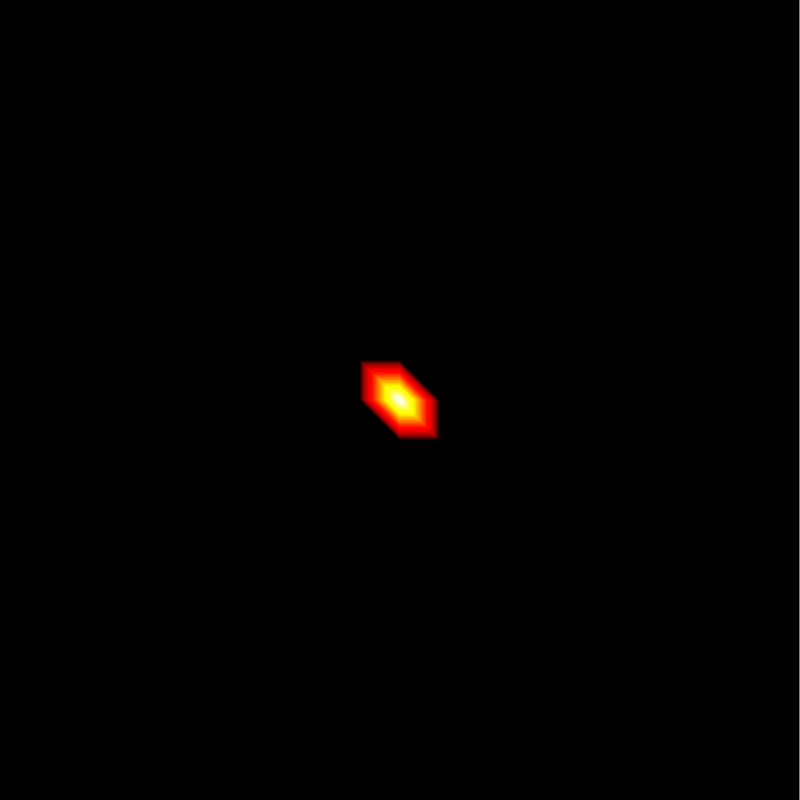
\includegraphics[width=1.0\linewidth,height=0.32\textheight,keepaspectratio]{data/synthetic_meshes/square_tessellation_2tri_Dirac_delta_10_v441_f800_funcvals_0iter.png}
		\caption{Sq2 v441\_f800 iter 0}\label{fig:sq2.d}
	\end{subfigure}

	\bigskip
	\begin{subfigure}[b]{0.48\linewidth}
		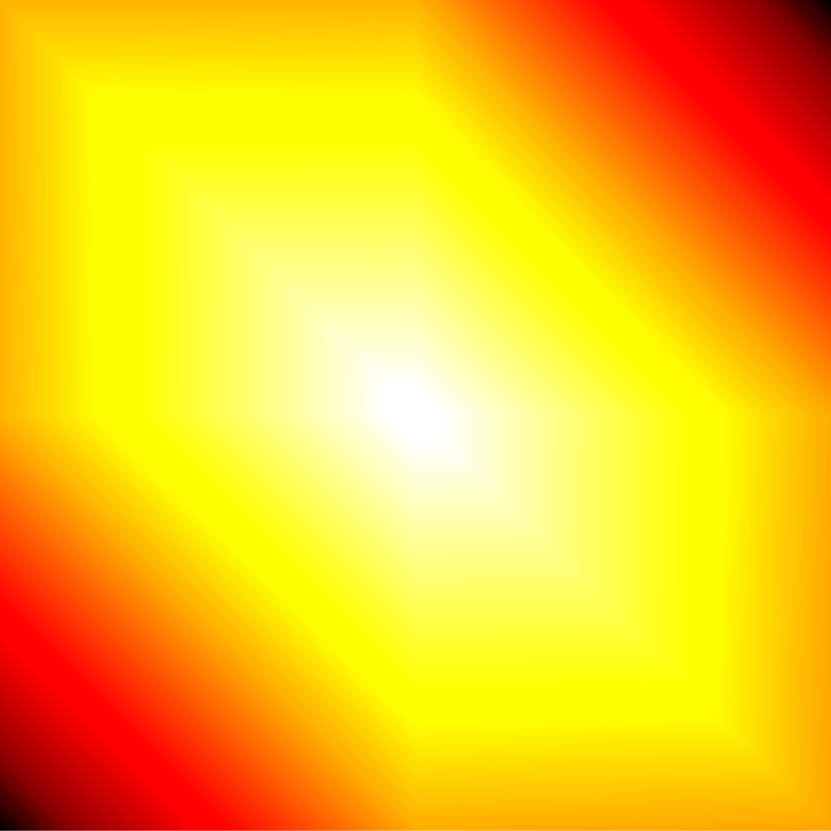
\includegraphics[width=1.0\linewidth,height=0.32\textheight,keepaspectratio]{data/synthetic_meshes/square_tesselation_2tri_Dirac_delta_1_v9_f8_funcvals_1iter_crop.png}
		\caption{Sq2 v9\_f8 iter 1}\label{fig:sq2.e}
	\end{subfigure}
	\begin{subfigure}[b]{0.48\linewidth}
		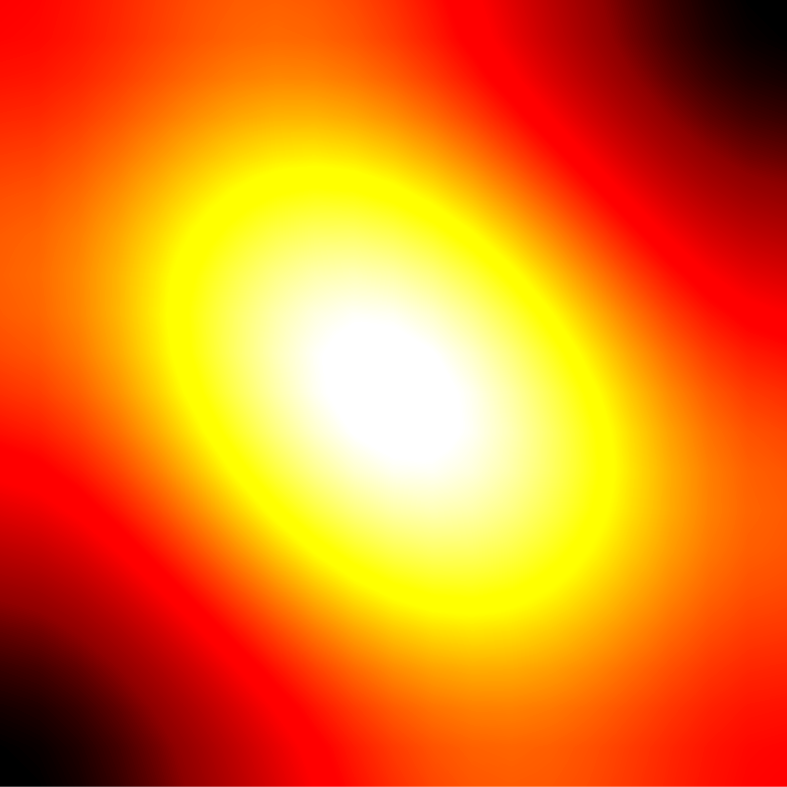
\includegraphics[width=1.0\linewidth,height=0.32\textheight,keepaspectratio]{data/synthetic_meshes/square_tessellation_2tri_Dirac_delta_10_v441_f800_funcvals_100iter.png}
		\caption{Sq2 v441\_f800 iter 100}\label{fig:sq2.f}
	\end{subfigure}}
	{\caption[Synthetic Square, 2 triangles, Dirac delta function]{A synthetic square, subdivided by triangles, with a Dirac delta function applied: (a) wireframe (b) colored by function value before filter (c) colored by function value after 1000 iterations
%GigaMesh~\cite{Mara10} with function values colored with the Improved Hot colorramp, exported as png after disabling the background grid [f7], maximizing the window, disabling screenshot cropping, as well as rejecting tiled rendering, finally cropping to content in GIMP.
	}\label{fig:sq2}}
\end{figure}
\todoCitation{}
\todoResearch{Why does sq2 10 need 100 iters to match sq 1 at 1 iters?}
\todoStyle{Why does sq2 1 iters 0 get differnt spacing?}
\todoStyle{Adjusting height, shrinks width => images no longer centered in their columns}

\subsubsection{Square grid, four triangles}

\subsubsection{Hexagonal grid}
\begin{figure}[ht]
\ffigbox
	{\begin{subfigure}[b]{0.48\linewidth}
		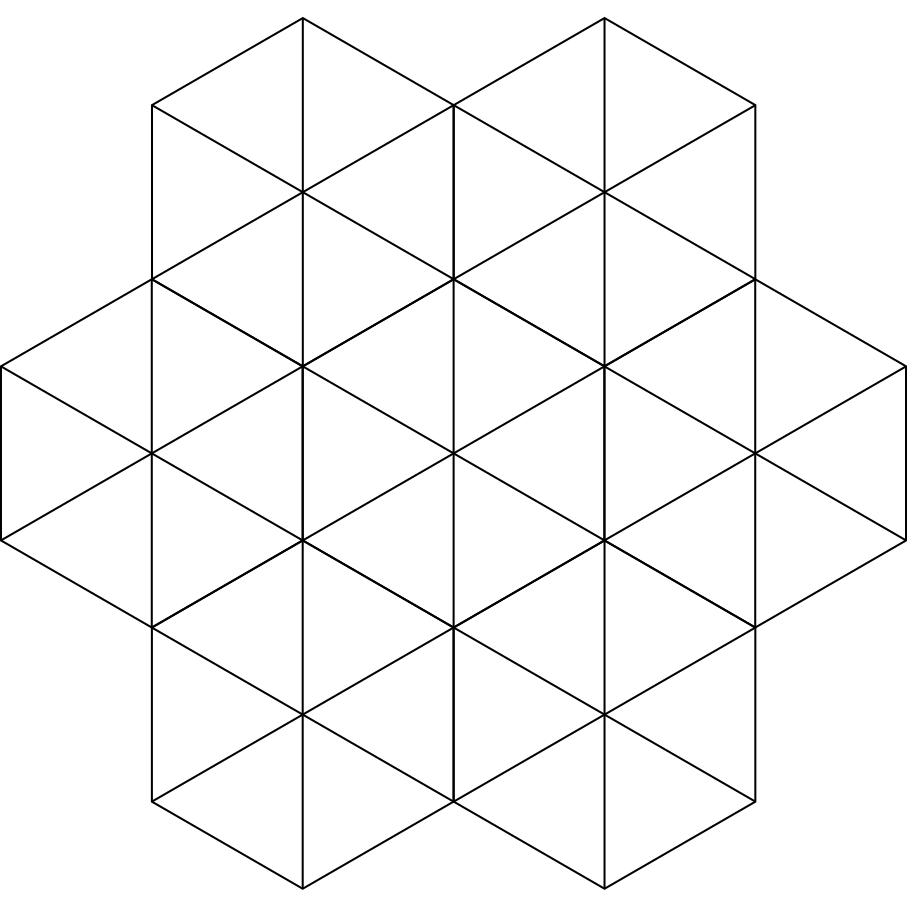
\includegraphics[width=1.0\linewidth,height=0.3\textheight,keepaspectratio]{data/synthetic_meshes/hexagonal_tessellation_Dirac_delta_1_v31_f42_wireframe.png}
		\caption{Hex v31\_f42 wireframe}\label{fig:hex.a}
	\end{subfigure}
	\begin{subfigure}[b]{0.48\linewidth}
		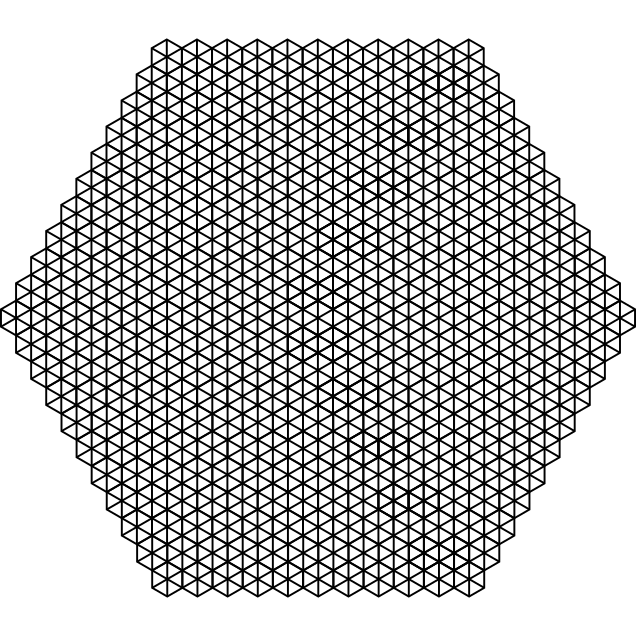
\includegraphics[width=1.0\linewidth,height=0.3\textheight,keepaspectratio]{data/synthetic_meshes/hexagonal_tessellation_Dirac_delta_10_v1057_f1986_wireframe.png}
		\caption{Hex v1057\_f1986 wireframe}\label{fig:hex.b}
	\end{subfigure}

	\bigskip
	\begin{subfigure}[b]{0.48\linewidth}
		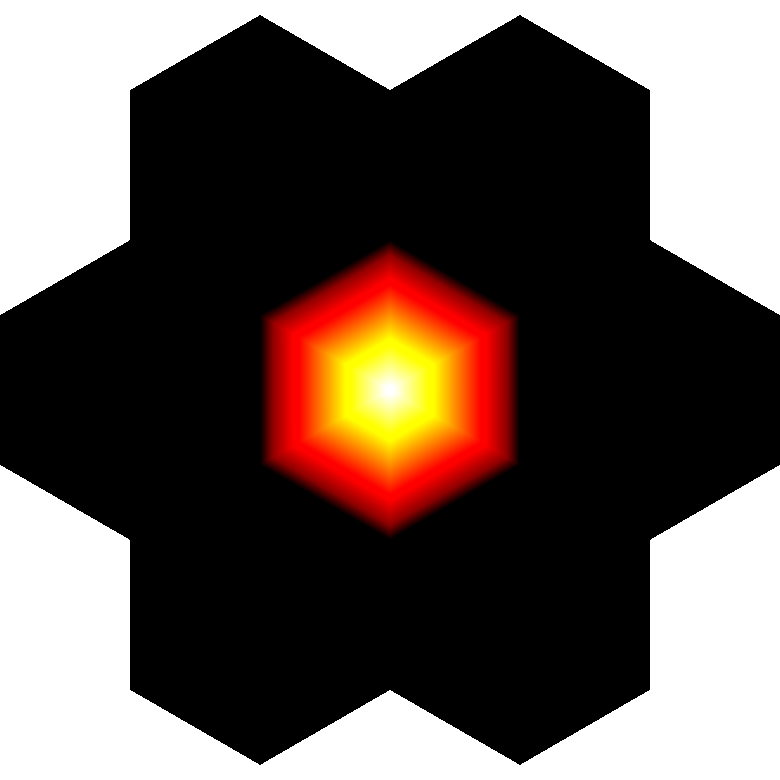
\includegraphics[width=1.0\linewidth,height=0.3\textheight,keepaspectratio]{data/synthetic_meshes/hexagonal_tessellation_Dirac_delta_1_v31_f42_funcvals_0iter_crop.png}
		\caption{Hex v31\_f42 iter 0}\label{fig:hex.c}
	\end{subfigure}
	\begin{subfigure}[b]{0.48\linewidth}
		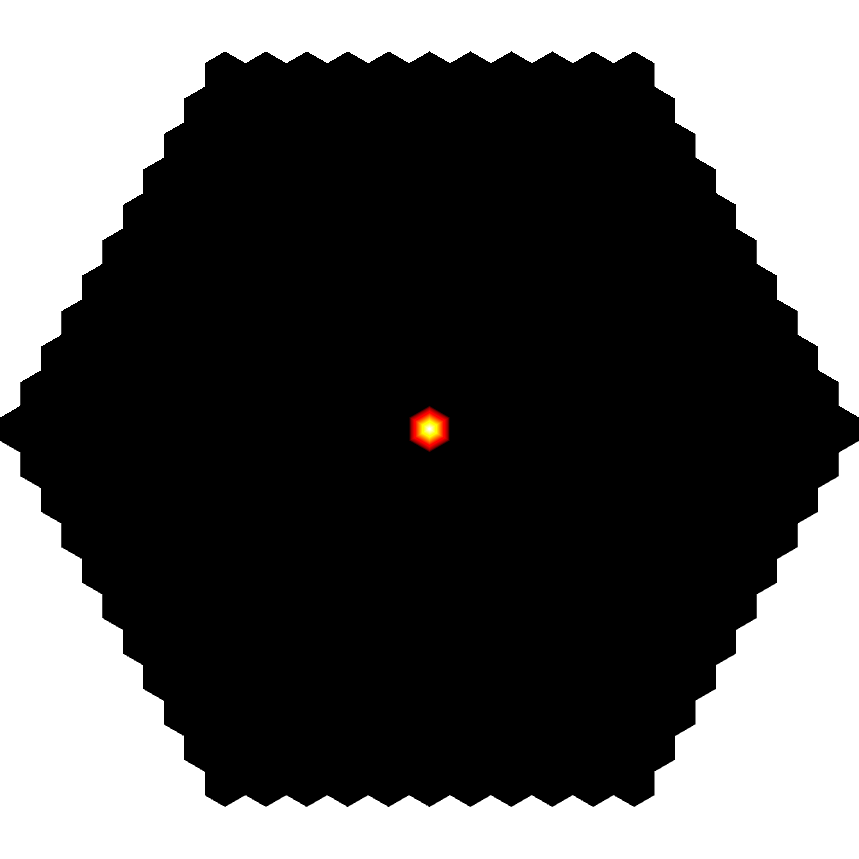
\includegraphics[width=1.0\linewidth,height=0.3\textheight,keepaspectratio]{data/synthetic_meshes/hexagonal_tessellation_Dirac_delta_10_v1057_f1986_funcvals_0iter_crop.png}
		\caption{Hex v1057\_f1986 iter 0}\label{fig:hex.d}
	\end{subfigure}

	\bigskip
	\begin{subfigure}[b]{0.48\linewidth}
		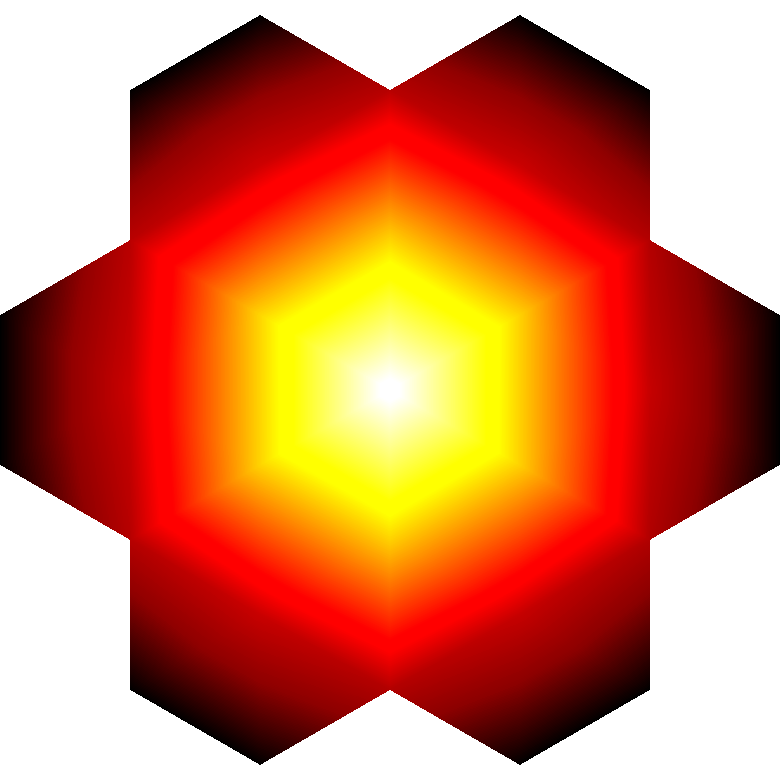
\includegraphics[width=1.0\linewidth,height=0.3\textheight,keepaspectratio]{data/synthetic_meshes/hexagonal_tessellation_Dirac_delta_1_v31_f42_funcvals_2iter_crop.png}
		\caption{Hex v31\_f42 iter 2}\label{fig:hex.e}
	\end{subfigure}
	\begin{subfigure}[b]{0.48\linewidth}
		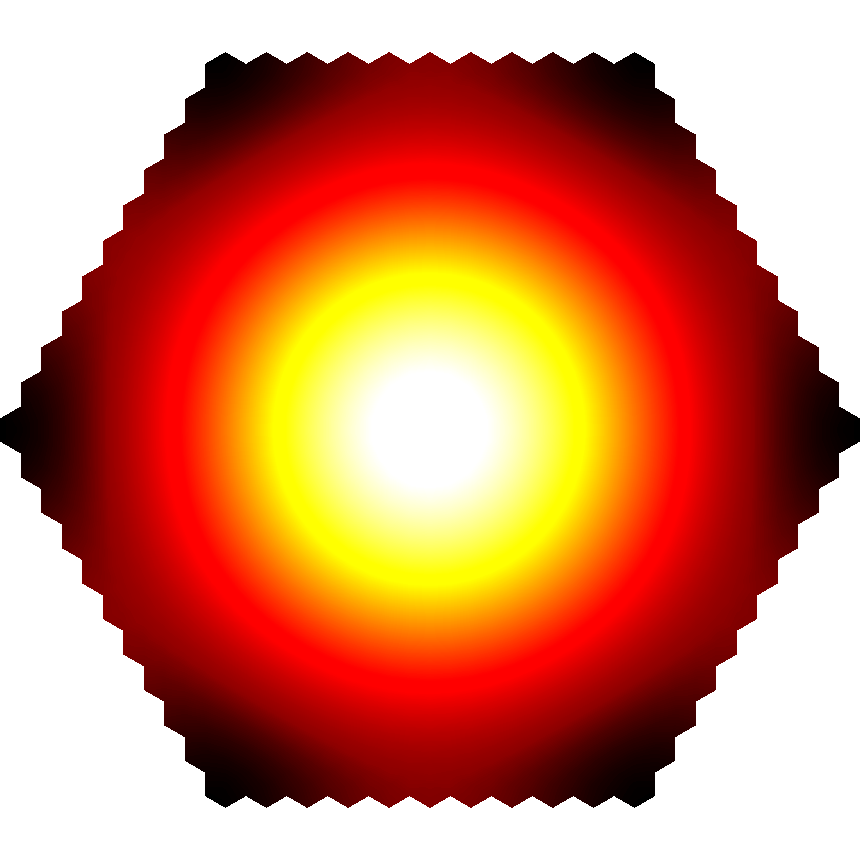
\includegraphics[width=1.0\linewidth,height=0.3\textheight,keepaspectratio]{data/synthetic_meshes/hexagonal_tessellation_Dirac_delta_10_v1057_f1986_funcvals_200iter_crop.png}
		\caption{Hex v1057\_f1986 iter 200}\label{fig:hex.f}
	\end{subfigure}}
	{\caption[Synthetic Hexagonal Tessellations, Dirac delta function]{A synthetic hexagonal tessellation, subdivided by triangles, with a Dirac delta function applied: (a) v31 f42 wireframe (b) v1057 f1986 wireframe (c) v31 f42 colored by function value before filter (d) v1057 f1986 colored by function value before filter (e) v31 f42 colored by function value after 2 iterations (e) v1057 f1986 colored by function value after 200 iterations.
% All using the colorramp "Hot (improved)"~\cite[p.~???]{Brewer2003}~\cite[p.~19]{Giga17}, visualized using GigaMesh~\cite{Mara10}, exported as png after disabling the background grid [f7], maximizing the window, disabling screenshot cropping, as well as rejecting tiled rendering, finally cropping to content in GIMP.
	}\label{fig:hex}}
\end{figure}
\todoCitation{}

\subsubsection{Random vertices within a circle}
\begin{figure}[ht]
\ffigbox
	{\begin{subfigure}[b]{0.48\linewidth}
		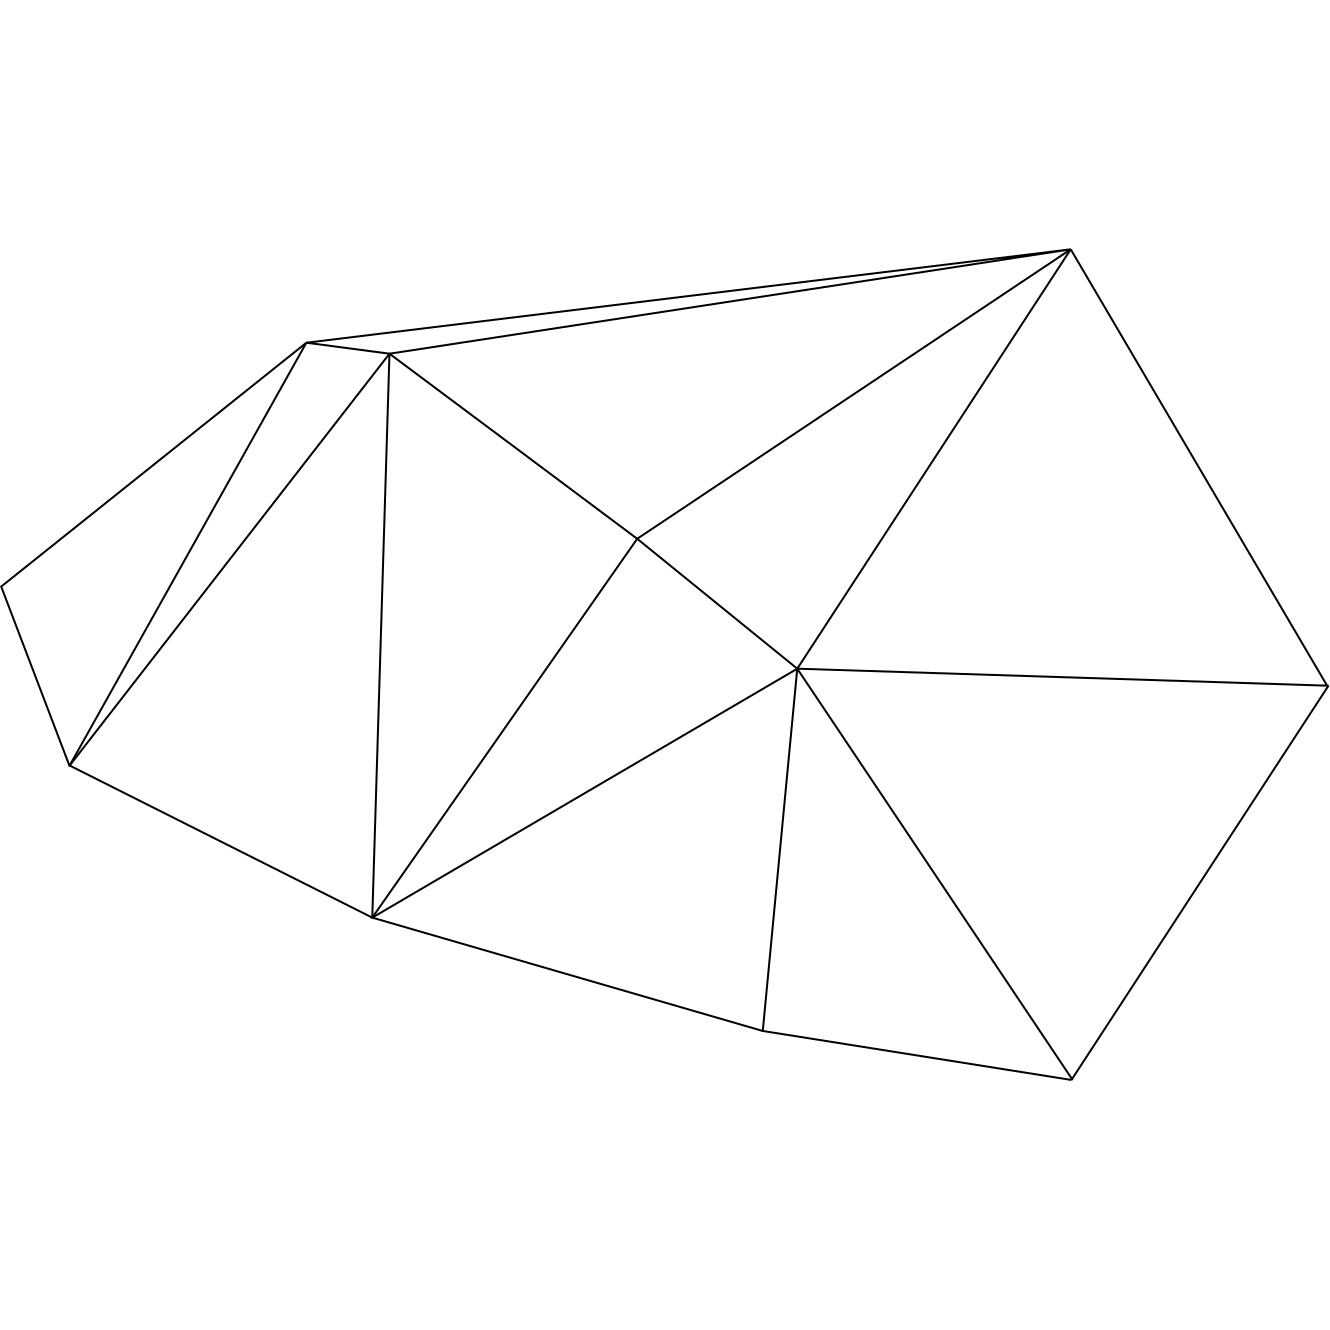
\includegraphics[width=1.0\linewidth,height=0.3\textheight,keepaspectratio]{data/synthetic_meshes/random_circle_tessellation_Dirac_delta_1_v11_f12_wireframe.png}
		\caption{R.Circ v11\_f12 wireframe}\label{fig:rcirc.a}
	\end{subfigure}
	\begin{subfigure}[b]{0.48\linewidth}
		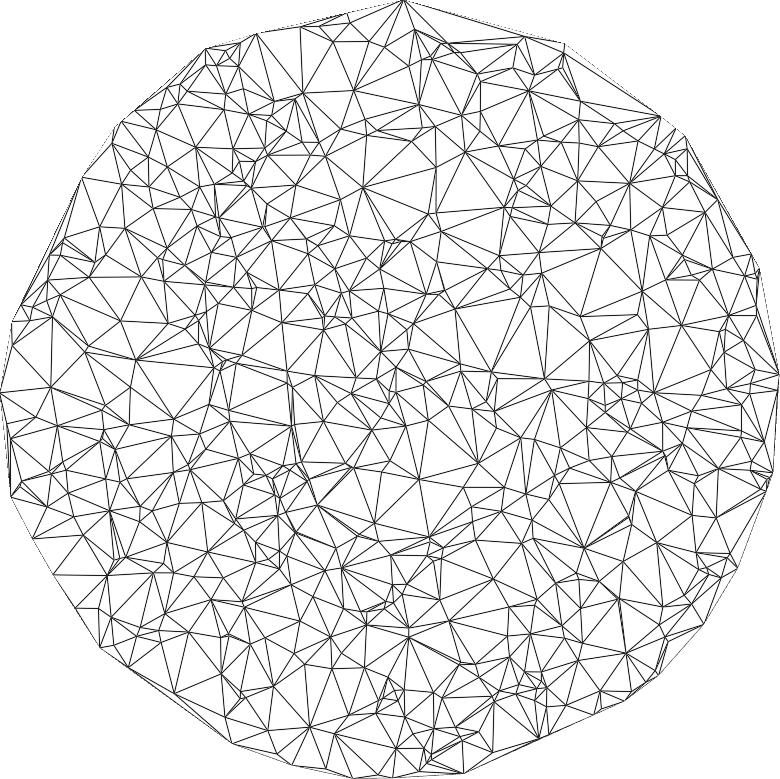
\includegraphics[width=1.0\linewidth,height=0.3\textheight,keepaspectratio]{data/synthetic_meshes/random_circle_tessellation_Dirac_delta_10_v641_f1252_wireframe.png}
		\caption{R.Circ v641\_f1252 wireframe}\label{fig:rcirc.b}
	\end{subfigure}

	\bigskip
	\begin{subfigure}[b]{0.48\linewidth}
		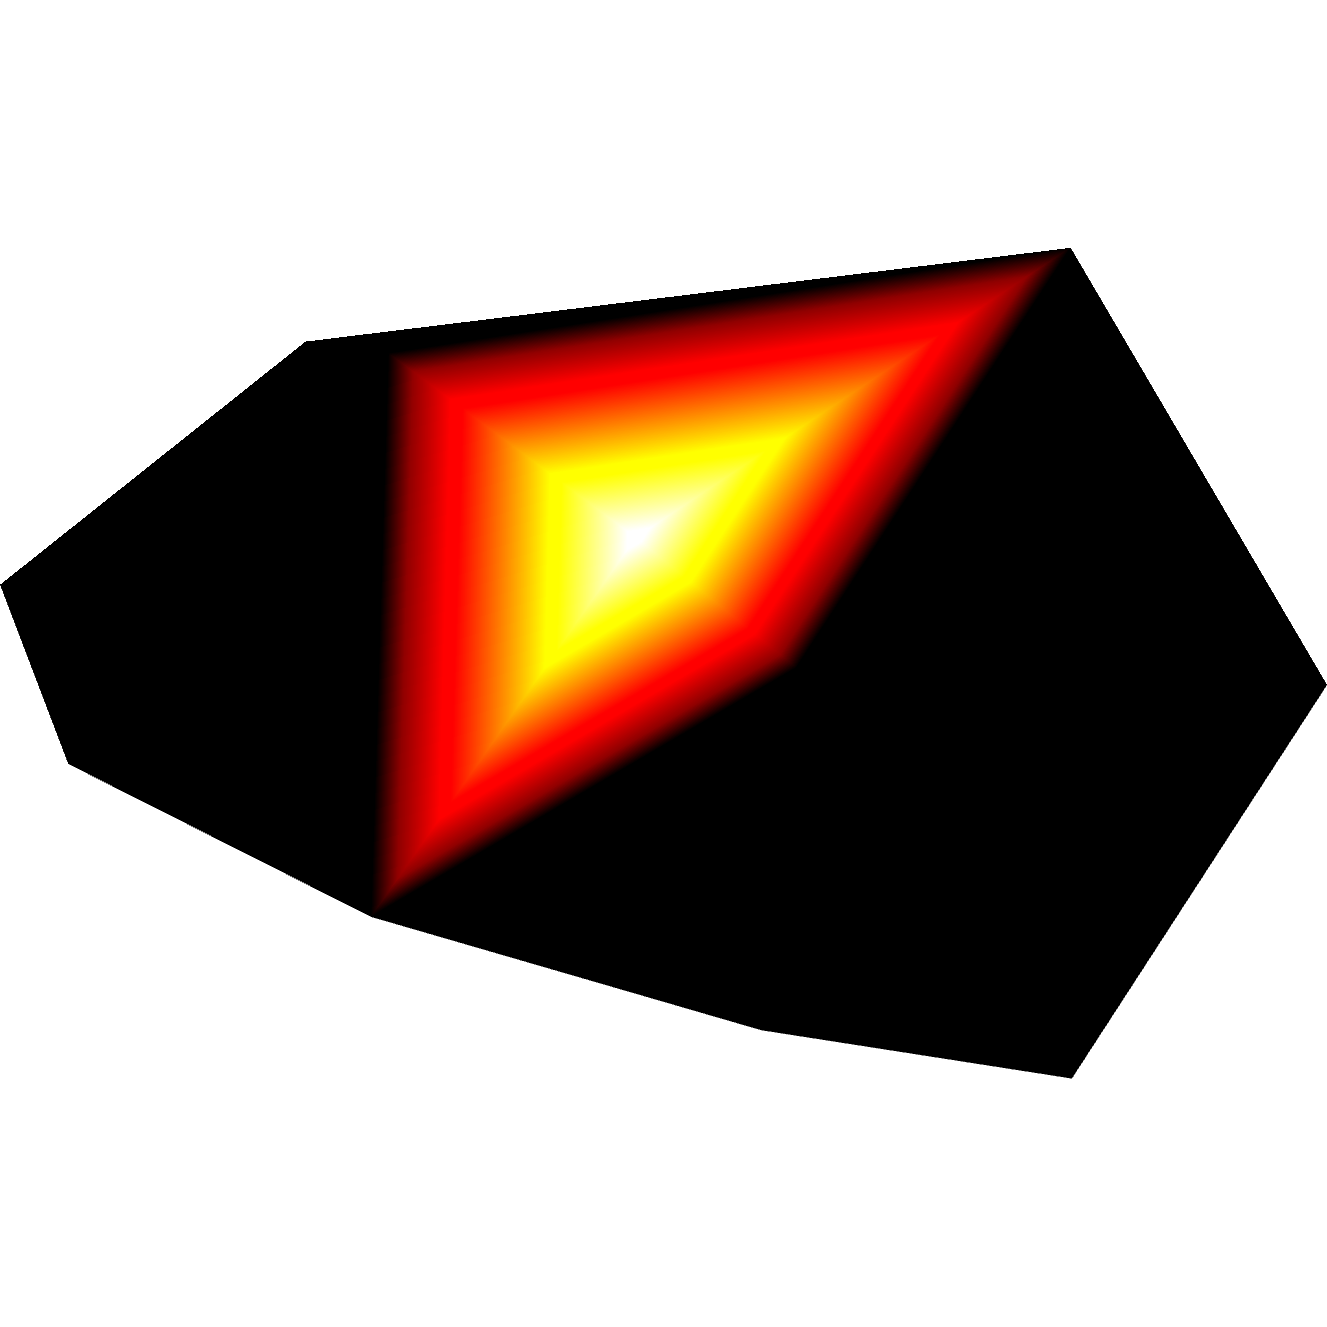
\includegraphics[width=1.0\linewidth,height=0.3\textheight,keepaspectratio]{data/synthetic_meshes/random_circle_tessellation_Dirac_delta_1_v11_f12_funcvals_0iter.png}
		\caption{R.Circ v11\_f12 iter 0}\label{fig:rcirc.c}
	\end{subfigure}
	\begin{subfigure}[b]{0.48\linewidth}
		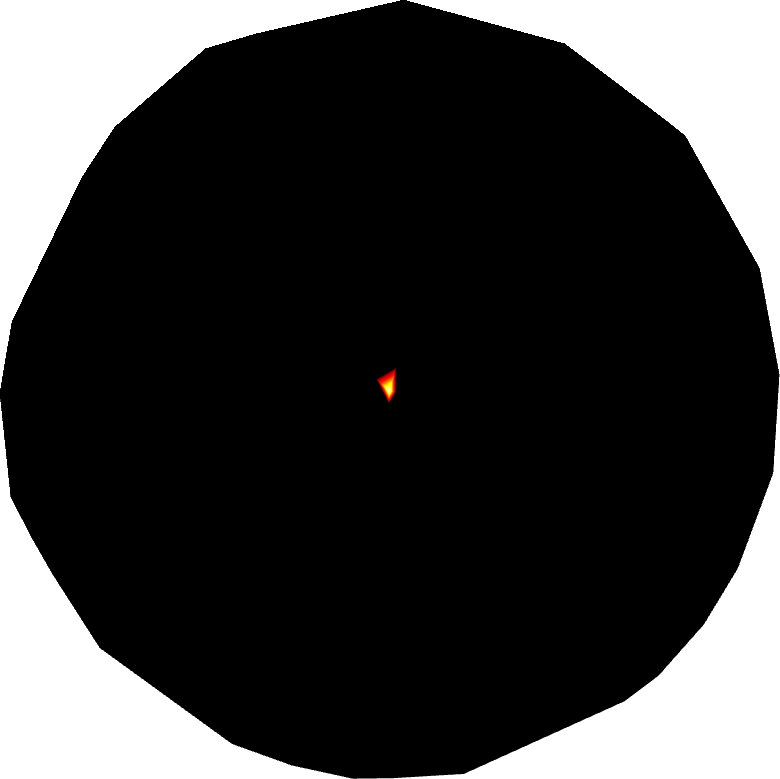
\includegraphics[width=1.0\linewidth,height=0.3\textheight,keepaspectratio]{data/synthetic_meshes/random_circle_tessellation_Dirac_delta_10_v641_f1252_funcvals_0iter.png}
		\caption{R.Circ v641\_f1252 iter 0}\label{fig:rcirc.d}
	\end{subfigure}

	\bigskip
	\begin{subfigure}[b]{0.48\linewidth}
		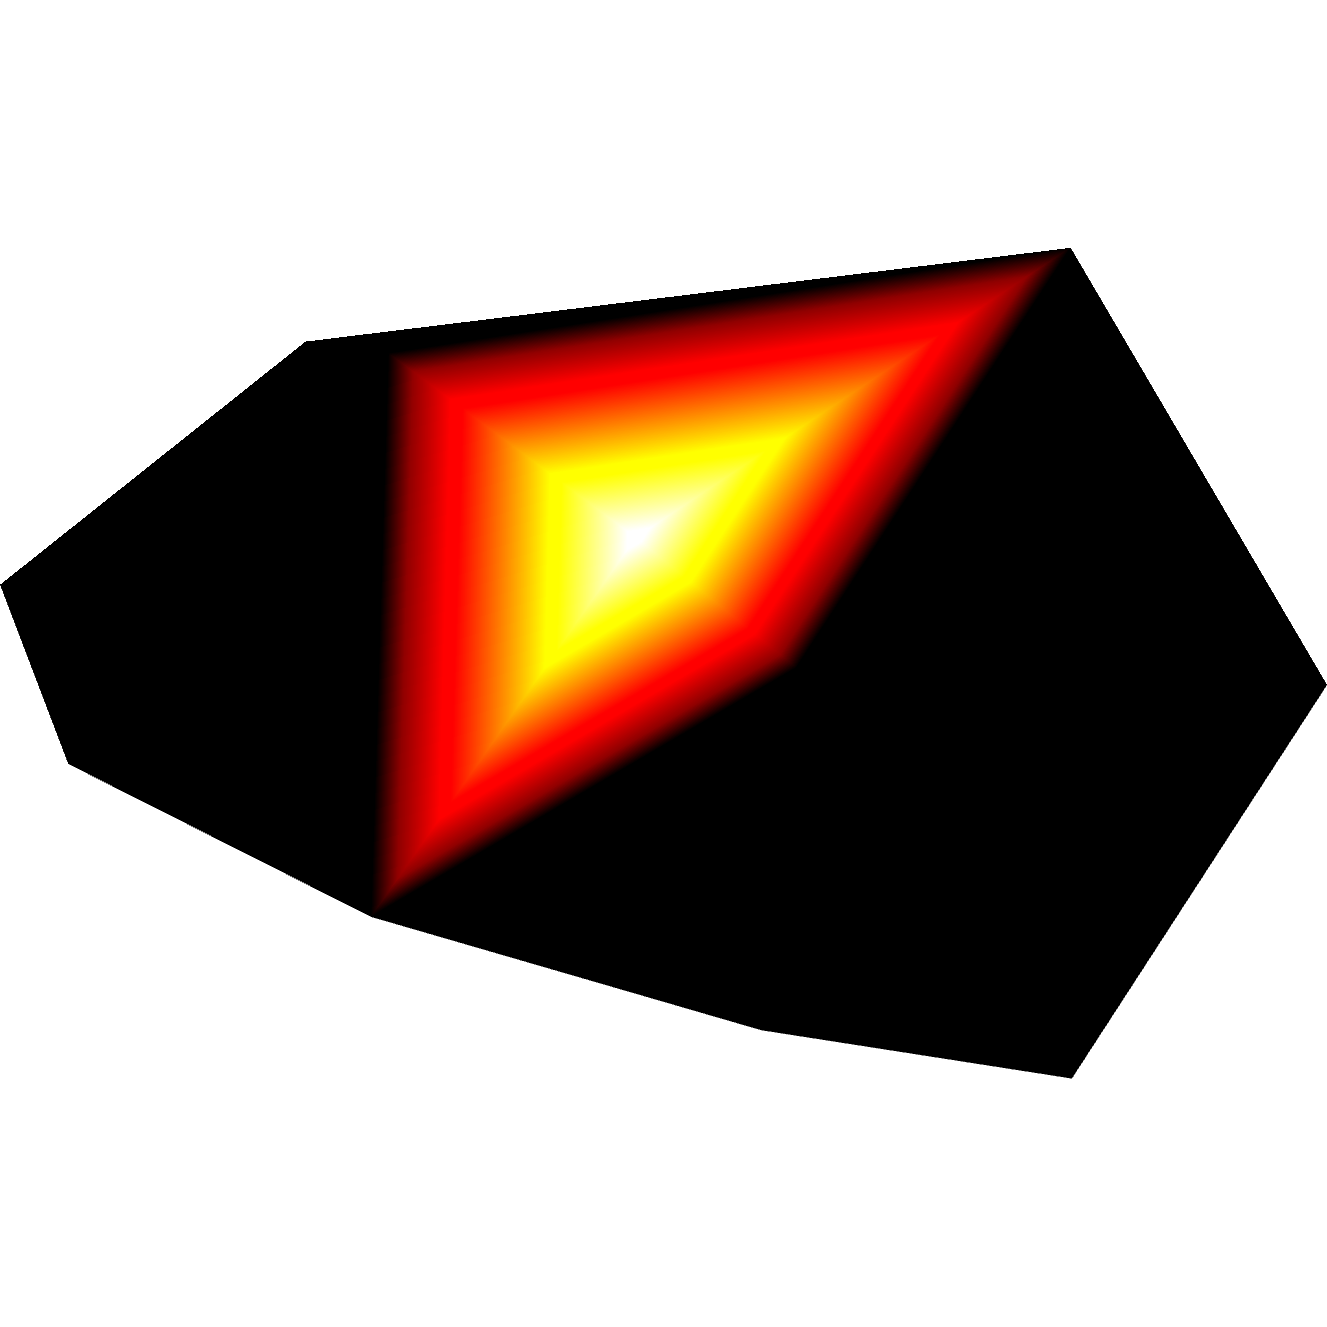
\includegraphics[width=1.0\linewidth,height=0.3\textheight,keepaspectratio,height=0.3\textheight,keepaspectratio]{data/synthetic_meshes/random_circle_tessellation_Dirac_delta_1_v11_f12_funcvals_0iter.png}
		\caption{R.Circ v11\_f12 iter 2}\label{fig:rcirc.e}
	\end{subfigure}
	\begin{subfigure}[b]{0.48\linewidth}
		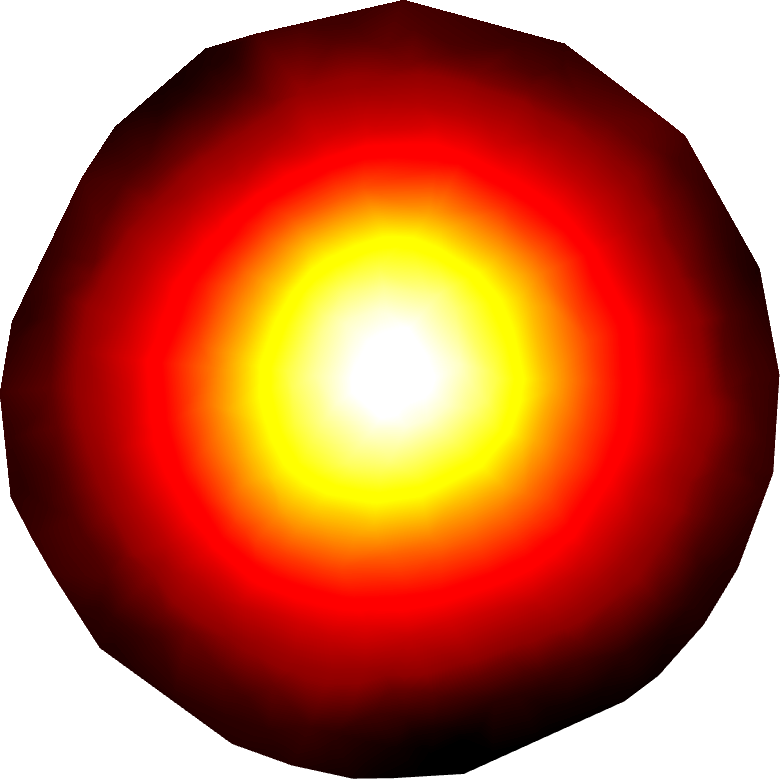
\includegraphics[width=1.0\linewidth,height=0.3\textheight,keepaspectratio,height=0.3\textheight,keepaspectratio]{data/synthetic_meshes/random_circle_tessellation_Dirac_delta_10_v641_f1252_funcvals_10000iter.png}
		\caption{R.Circ v641\_f1252 iter 10,000}\label{fig:rcirc.f}
	\end{subfigure}}
	{\caption[Synthetic random vertices equally distributed per radius, Dirac delta function]{A synthetic circle filled with random vertices equaly distributed per radius, triangulated by Delauney method~\cite[p.~??]{todoCitation}, with a Dirac delta function applied: (a) v11\_f12 wireframe (b) v641\_f1252 wireframe (c) v11\_f12 colored by function value before filter (d) v641\_f1252 colored by function value before filter (e) v11\_f12 colored by function value after 2 iterations (f) v641\_f1252 colored by function value after 10,000 iterations.
%All using the colorramp "Hot (improved)"~\cite[p.~???]{Brewer2003}~\cite[p.~19]{Giga17}, visualized using GigaMesh~\cite{Mara10}, exported as png after disabling the background grid [f7], maximizing the window, disabling screenshot cropping, as well as rejecting tiled rendering, finally cropping to content in GIMP.
}\label{fig:rcirc}}
\end{figure}
\todoCitation{}
\todoResearch{Why and who equally distributed}

%\subsection{Debossed H}
%In Figure \ref{fig:h}, we show a debossed capital letter H.\footnote{The H is
%as a nod to Heidelberg University and the cuniform script studied by the FCGL.}
%\begin{figure}[ht]
%\centering
%	\begin{subfigure}{.48\linewidth}
%		\centering
%		\resizebox{0.48\linewidth}{!}{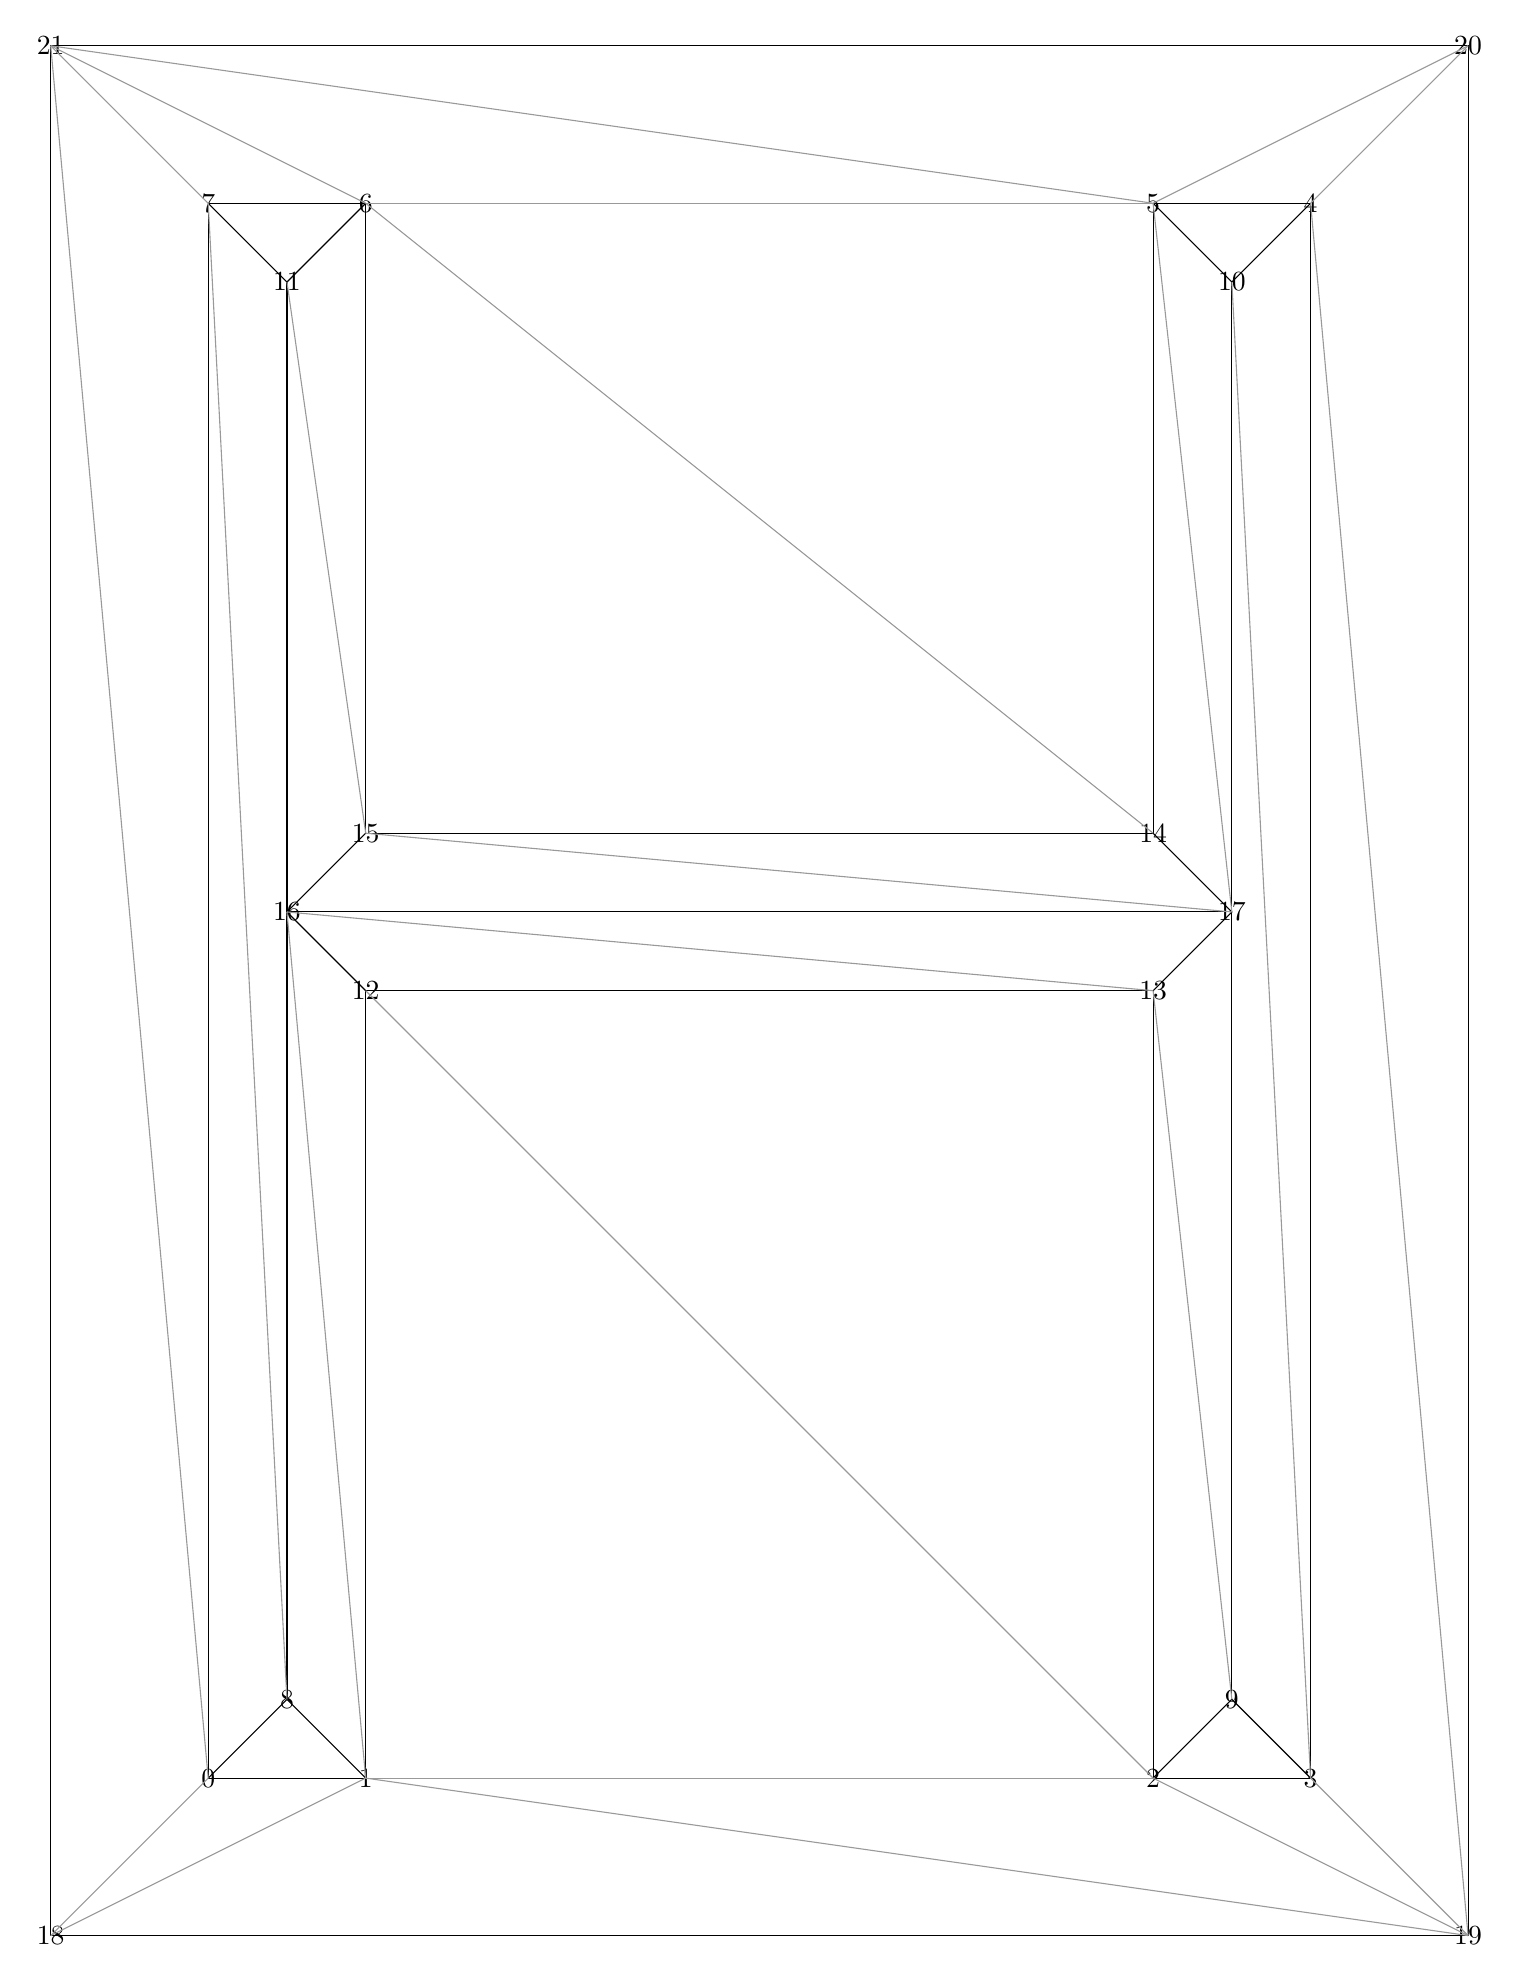
\begin{tikzpicture}
% Colors
\definecolor{outlineColor}{RGB}{0,0,0}
\definecolor{supportColor}{RGB}{153,153,153}
% Main H shape and Outline
\begin{scope}[outlineColor]
	\draw( 0, 0) node  {0} % 0
	  -- ( 2, 0) node  {1} % 1
	  -- ( 2,10) node {12} %12
	  -- (12,10) node {13} %13
	  -- (12, 0) node  {2} % 2
	  -- (14, 0) node  {3} % 3
	  -- (14,20) node  {4} % 4
	  -- (12,20) node  {5} % 5
	  -- (12,12) node {14} %14
	  -- ( 2,12) node {15} %15
	  -- ( 2,20) node  {6} % 6
	  -- ( 0,20) node  {7} % 7
	  -- cycle;  
	\draw( 0, 0) % 0
	  -- ( 1, 1) node  {8} % 8
	  -- ( 2, 0);% 1
	\draw(12, 0) % 2
	  -- (13, 1) node  {9} % 9
	  -- (14, 0);% 3
	\draw(14,20) % 4
	  -- (13,19) node {10} %10
	  -- (12,20);% 5
	\draw( 2,20) % 6
	  -- ( 1,19) node {11} %11
	  -- ( 0,20);% 7
	\draw( 2,10) %12
	  -- ( 1,11) node {16} %16
	  -- ( 2,12);%15
	\draw(12,10) %13
	  -- (13,11) node {17} %17
	  -- (12,12);%14
	\draw( 1, 1) % 8
	  -- ( 1,19);%11
	\draw(13, 1) % 9
	  -- (13,19);%10
	\draw( 1,11) %16
	  -- (13,11);%17
	\draw(-2,-2) node {18} %18
	  -- (16,-2) node {19} %19
	  -- (16,22) node {20} %20
	  -- (-2,22) node {21} %21
	  -- cycle;
\end{scope}
\begin{scope}[supportColor, thin]
	\draw( 0, 0) -- (-2,-2); % 0--18
	\draw( 0, 0) -- (-2,22); % 0--21
	\draw( 2, 0) -- (12, 0); % 1-- 2
	\draw( 2, 0) -- ( 1,11); % 1--16
	\draw( 2, 0) -- (-2,-2); % 1--18
	\draw( 2, 0) -- (16,-2); % 1--19
	\draw(12, 0) -- ( 2,10); % 2--12
	\draw(12, 0) -- (16,-2); % 2--19
	\draw(14, 0) -- (13,19); % 3--10
	\draw(14, 0) -- (16,-2); % 3--19
	\draw(14,20) -- (16,-2); % 4--19
	\draw(14,20) -- (16,22); % 4--20
	\draw(12,20) -- ( 2,20); % 5-- 6
	\draw(12,20) -- (13,11); % 5--17
	\draw(12,20) -- (16,22); % 5--20
	\draw(12,20) -- (-2,22); % 5--21
	\draw( 2,20) -- (12,12); % 6--14
	\draw( 2,20) -- (-2,22); % 6--21
	\draw( 0,20) -- ( 1, 1); % 7-- 8
	\draw( 0,20) -- (-2,22); % 7--21
	\draw(13, 1) -- (12,10); % 9--13
	\draw( 1,19) -- ( 2,12); %11--15
	\draw(12,10) -- ( 1,11); %13--16
	\draw( 2,12) -- (13,11); %15--17
\end{scope}
\end{tikzpicture}
}
%		\caption{HWireframe}\label{fig:h.a}
%	\end{subfigure}
%	\hfill
%	\begin{subfigure}{.48\linewidth}
%		\centering
%		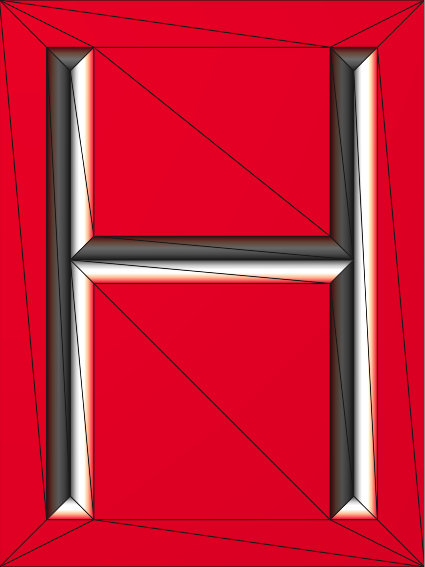
\includegraphics[width=0.48\linewidth]{data/synthetic_meshes/h_colored.png}
%		\caption{HColored}\label{fig:h.b}
%	\end{subfigure}
%	\caption[A debossed H, which contains 22 vertices and 36 faces.]{A debossed H,
%	which contains 22 vertices and 36 faces: (a) wireframe (b) colored by the
%	relation to its distance to an underlying plane, in RdGy
%	colorramp~\cite[p.~???]{Brewer2003}~\cite[p.~19]{Giga17}, visualized using the
%	GigaMesh~\cite{Mara10} framework with triangle edges rendered.}\label{fig:h}
%\end{figure}
To evaluate methods available for discrete surfaces, we can increase the number
of vertices of our synthetic wedge using five iterations of the mid-edge
subdivision scheme [PR97,
HW99].~\cite[p.~38]{Mara12}



\section{Acquired Data}
Acquired Data examples are actually recorded by sensors.
Something in Archaeology
Cuneiform Tablets
Mayan Tablets
Dynamic Earth models

\subsection{University Seal}
Unisiegel\_\- UAH\_\- Ebay-Siegel\_\- Uniarchiv\_\- HE2066-60\_\- 010614\_\- partial\_\- ASCII.ply
%\begin{figure}[ht]
%\ffigbox
%	{\begin{subfigure}[b]{0.48\linewidth}
%		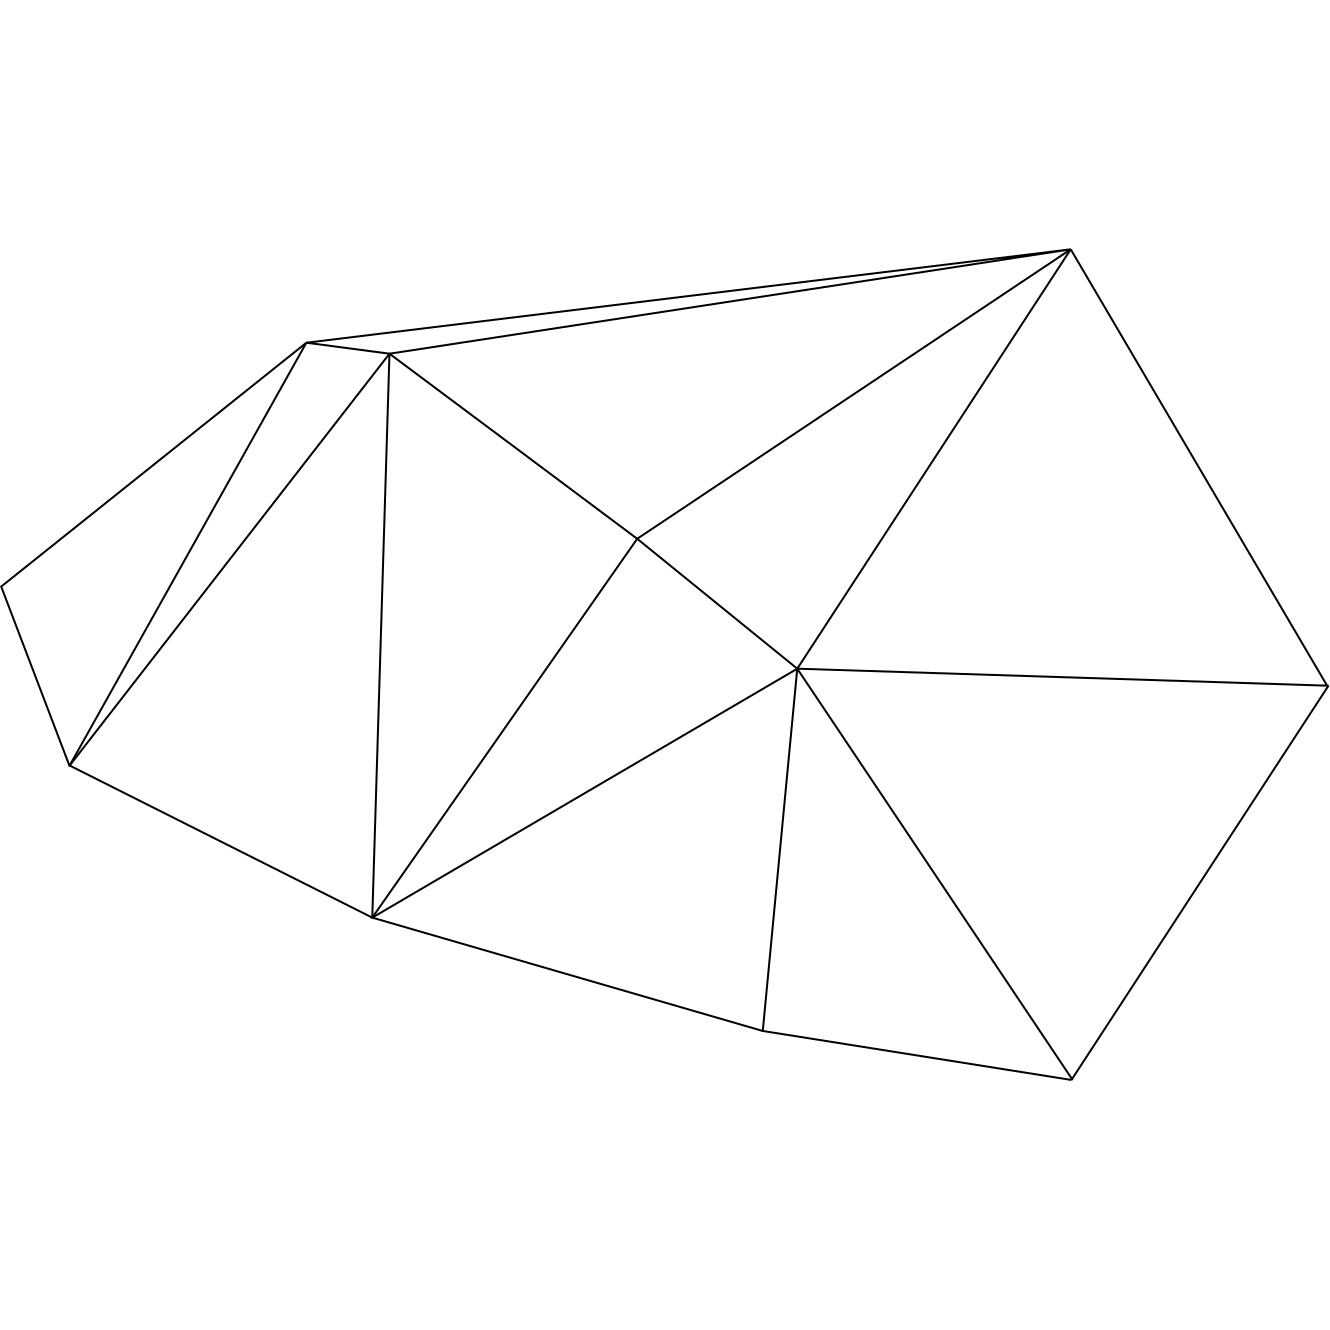
\includegraphics[width=1.0\linewidth,height=0.3\textheight,keepaspectratio]{data/synthetic_meshes/random_circle_tessellation_Dirac_delta_1_v11_f12_wireframe.png}
%		\caption{R.Circ v11\_f12 wireframe}\label{fig:rcirc.a}
%	\end{subfigure}
%	\begin{subfigure}[b]{0.48\linewidth}
%		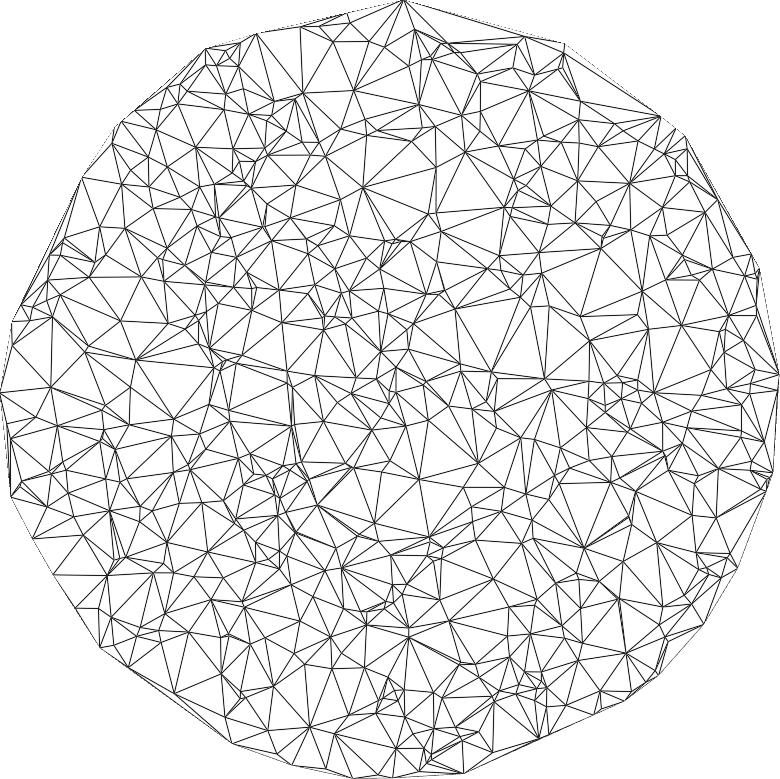
\includegraphics[width=1.0\linewidth,height=0.3\textheight,keepaspectratio]{data/synthetic_meshes/random_circle_tessellation_Dirac_delta_10_v641_f1252_wireframe.png}
%		\caption{R.Circ v641\_f1252 wireframe}\label{fig:rcirc.b}
%	\end{subfigure}
%
%	\bigskip
%	\begin{subfigure}[b]{0.48\linewidth}
%		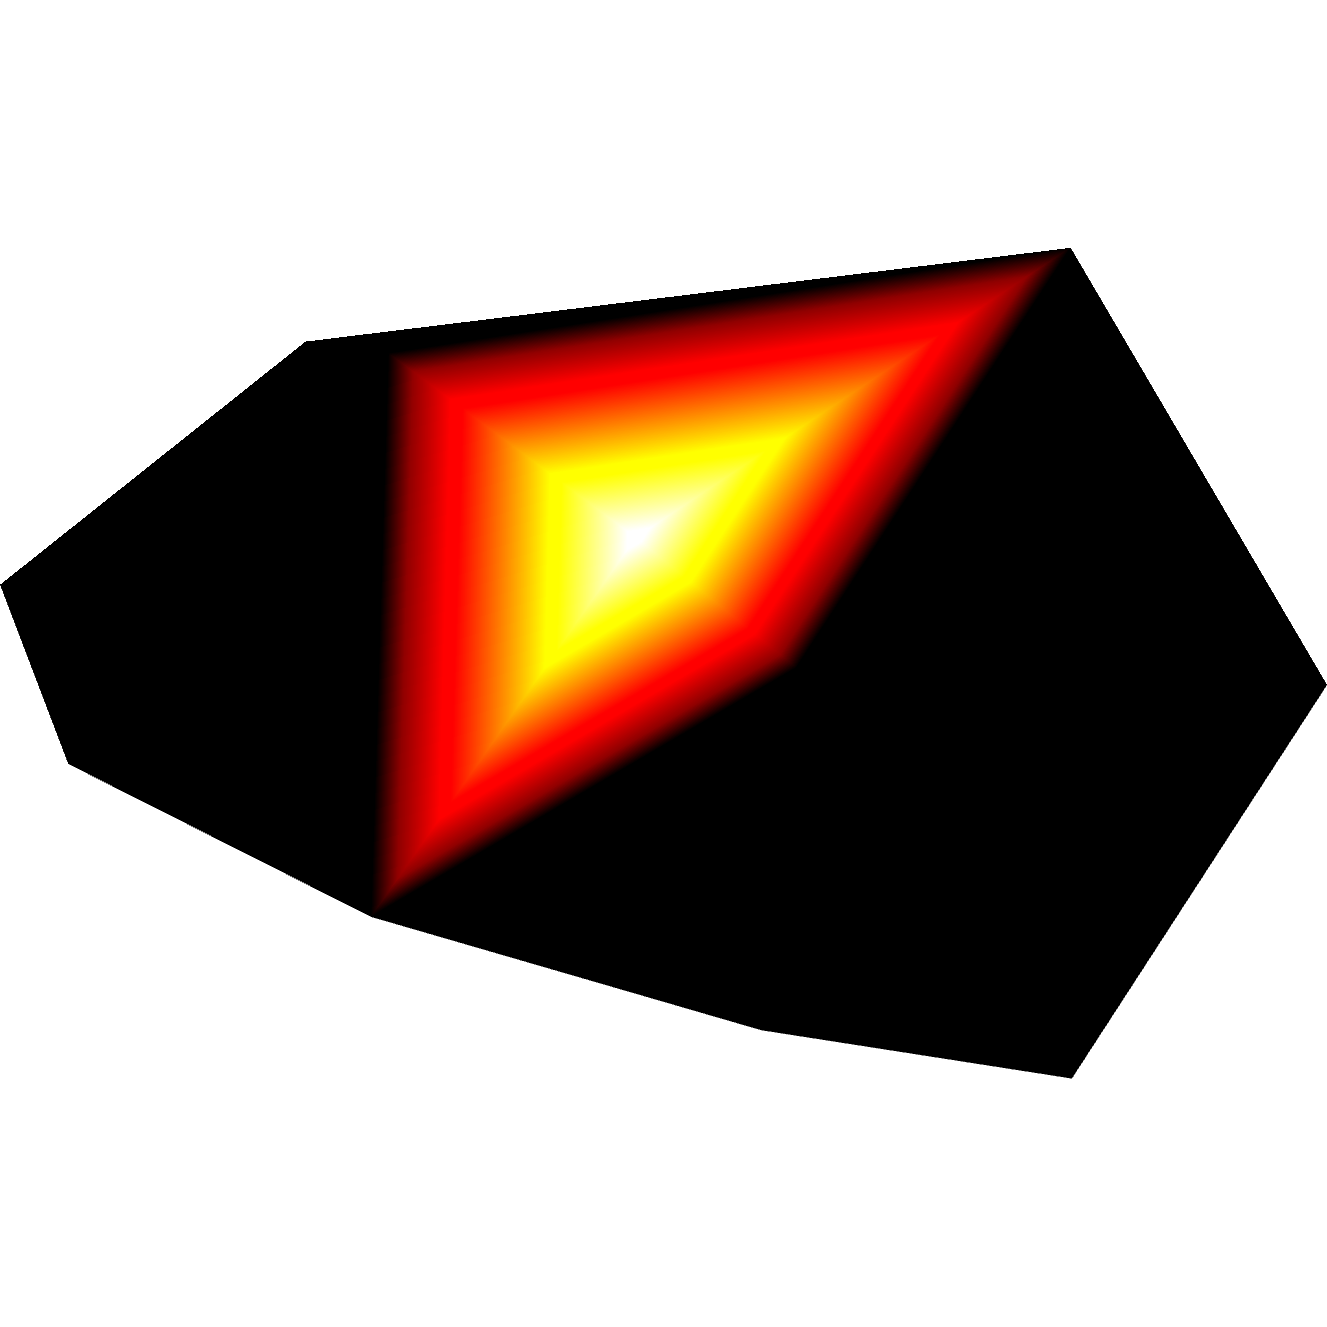
\includegraphics[width=1.0\linewidth,height=0.3\textheight,keepaspectratio]{data/synthetic_meshes/random_circle_tessellation_Dirac_delta_1_v11_f12_funcvals_0iter.png}
%		\caption{R.Circ v11\_f12 iter 0}\label{fig:rcirc.c}
%	\end{subfigure}
%	\begin{subfigure}[b]{0.48\linewidth}
%		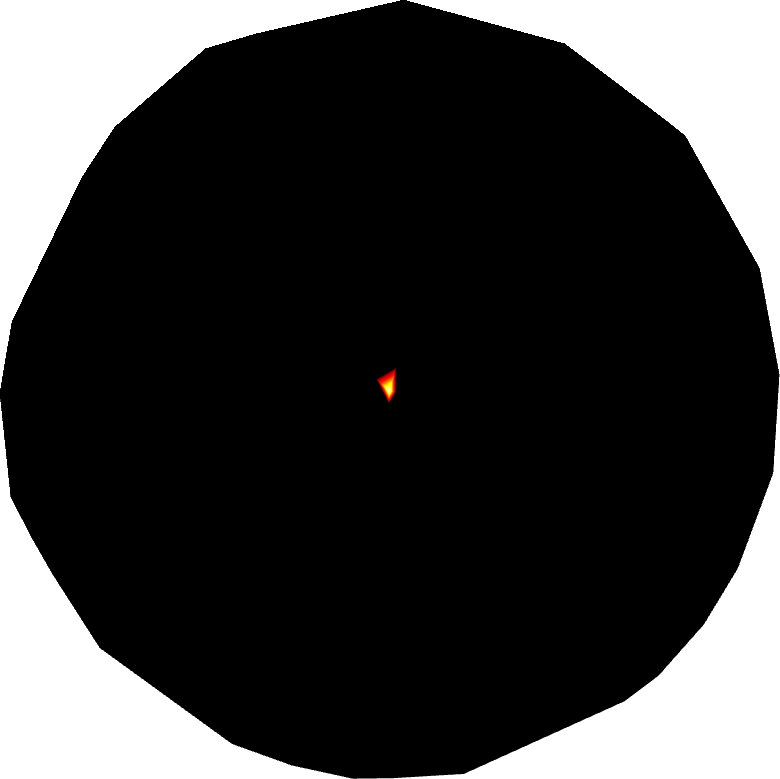
\includegraphics[width=1.0\linewidth,height=0.3\textheight,keepaspectratio]{data/synthetic_meshes/random_circle_tessellation_Dirac_delta_10_v641_f1252_funcvals_0iter.png}
%		\caption{R.Circ v641\_f1252 iter 0}\label{fig:rcirc.d}
%	\end{subfigure}
%
%	\bigskip
%	\begin{subfigure}[b]{0.48\linewidth}
%		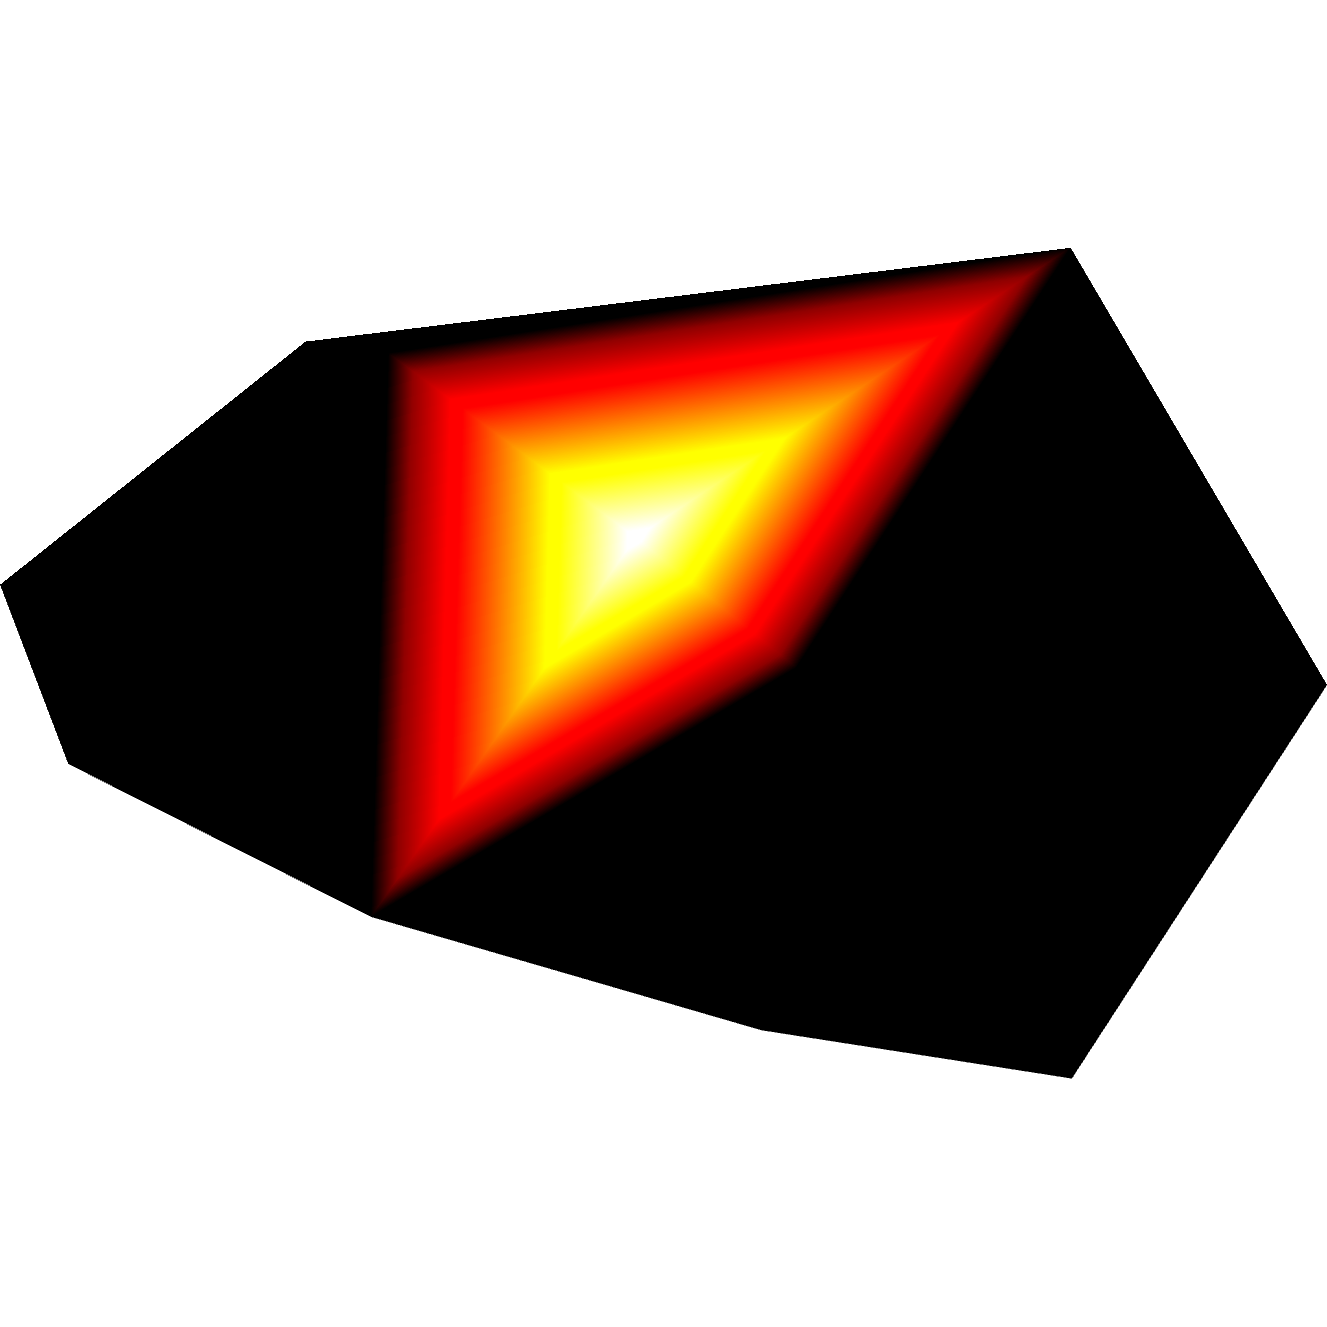
\includegraphics[width=1.0\linewidth,height=0.3\textheight,keepaspectratio]{data/synthetic_meshes/random_circle_tessellation_Dirac_delta_1_v11_f12_funcvals_0iter.png}
%		\caption{R.Circ v11\_f12 iter 2}\label{fig:rcirc.e}
%	\end{subfigure}
%	\begin{subfigure}[b]{0.48\linewidth}
%		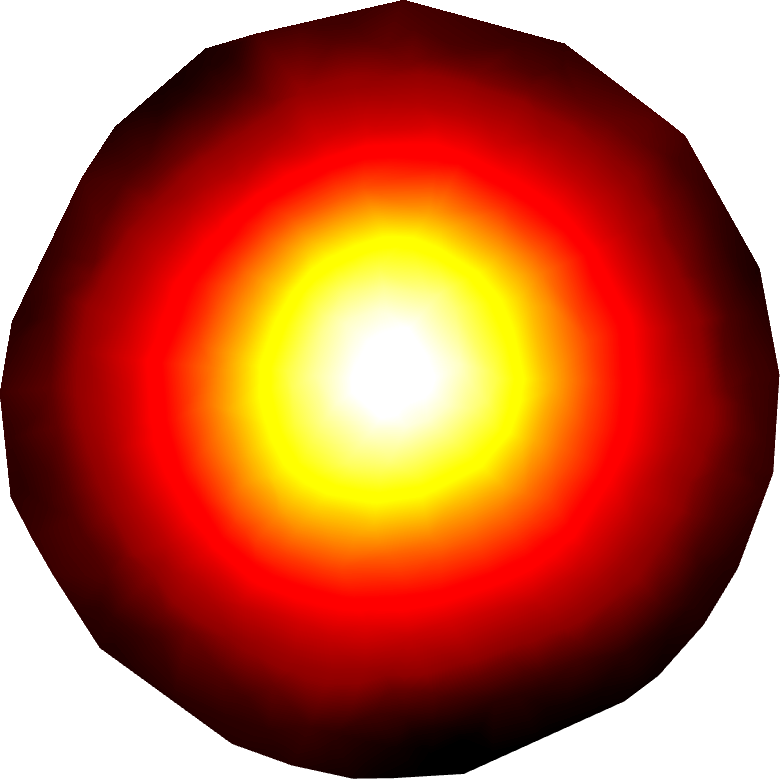
\includegraphics[width=1.0\linewidth,height=0.3\textheight,keepaspectratio]{data/synthetic_meshes/random_circle_tessellation_Dirac_delta_10_v641_f1252_funcvals_10000iter.png}
%		\caption{R.Circ v641\_f1252 iter 10,000}\label{fig:rcirc.f}
%	\end{subfigure}}
%	{\caption[Synthetic random vertices equally distributed per radius, Dirac delta function]{A synthetic circle filled with random vertices equaly distributed per radius, triangulated by Delauney method~\cite[p.~??]{todoCitation}, with a Dirac delta function applied: (a) v11\_f12 wireframe (b) v641\_f1252 wireframe (c) v11\_f12 colored by function value before filter (d) v641\_f1252 colored by function value before filter (e) v11\_f12 colored by function value after 2 iterations (f) v641\_f1252 colored by function value after 10,000 iterations.
%All using the colorramp "Hot (improved)"~\cite[p.~???]{Brewer2003}~\cite[p.~19]{Giga17}, visualized using GigaMesh~\cite{Mara10}, exported as png after disabling the background grid [f7], maximizing the window, disabling screenshot cropping, as well as rejecting tiled rendering, finally cropping to content in GIMP.
%}\label{fig:rcirc}}
%\end{figure}

\subsection{Mars Crater}
Mars dataset crater as a Digital Terrain Models (DTMs) Mention in Mara 3.6
Summary “Dali” inspired methodProcessing regular grids like Digital Terrain
Models (DTMs) will gain dramatic performance increases using the estimator,
while processing irregular grids with high curvatures will strongly benefit
from precise computation of the volume integral invariant.~\cite[p.~143]{Mara12}

\subsection{A Flat surface}
Flat surfaces have NOISE!
Figure~\ref{fig:ILATO}: ILATO\_1A\_SM2066-HE5-60\_070214\_merged\_GMO\_r1.00\_n4\_v256
\begin{figure}[ht]
\ffigbox
	{\begin{subfigure}[b]{0.48\linewidth}
		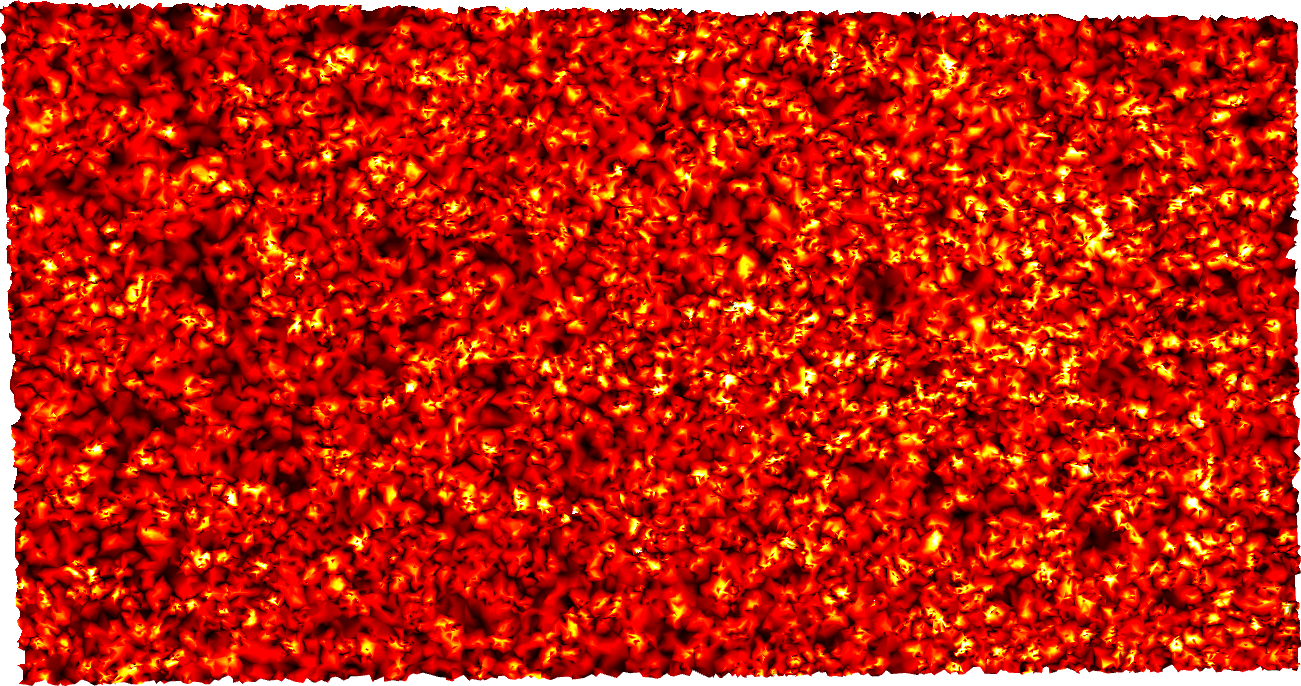
\includegraphics[width=1.0\linewidth,height=0.3\textheight,keepaspectratio]{data/acquired_meshes/ILATO_1A_SM2066-HE5-60_070214_merged_GMO_r1_n4_v256_funcvals_0iter.png}
		\caption{ILATO 0iter}\label{fig:ILATO.a}
	\end{subfigure}
	\begin{subfigure}[b]{0.48\linewidth}
		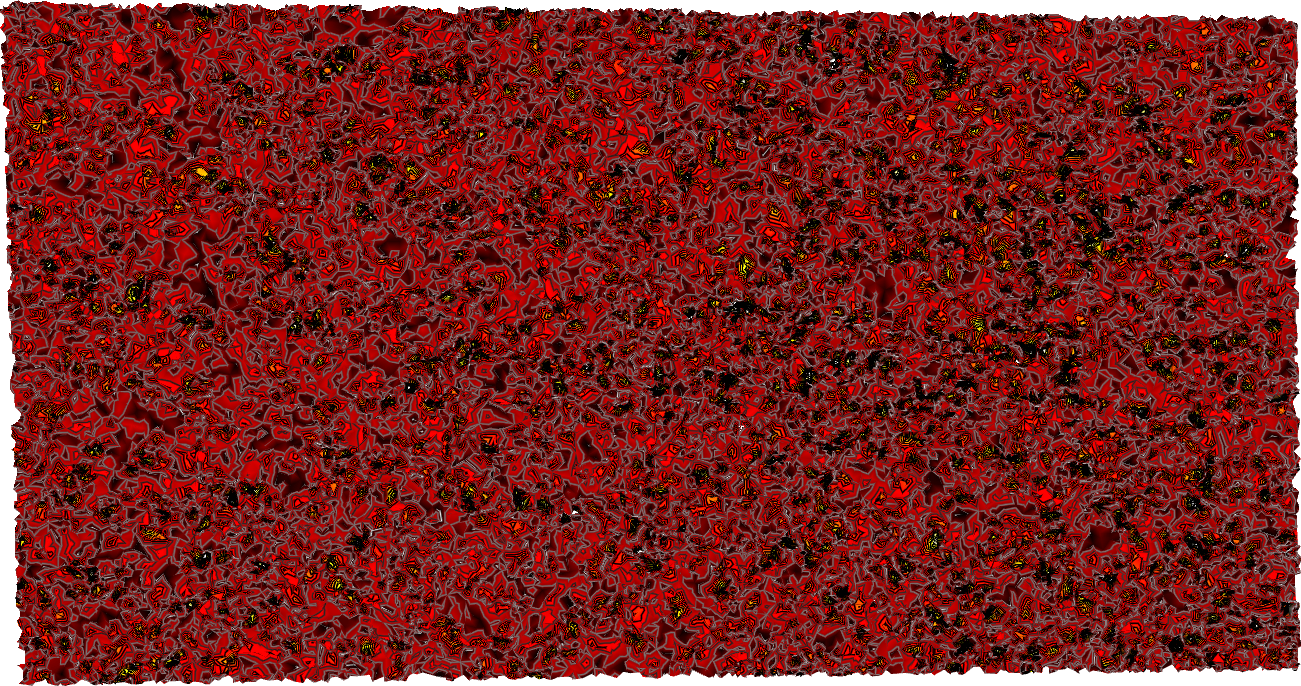
\includegraphics[width=1.0\linewidth,height=0.3\textheight,keepaspectratio]{data/acquired_meshes/ILATO_1A_SM2066-HE5-60_070214_merged_GMO_r1_n4_v256_funcvals_isolines_0iter.png}
		\caption{ILATO 0iter isolines}\label{fig:ILATO.b}
	\end{subfigure}

	\bigskip
	\begin{subfigure}[b]{0.48\linewidth}
		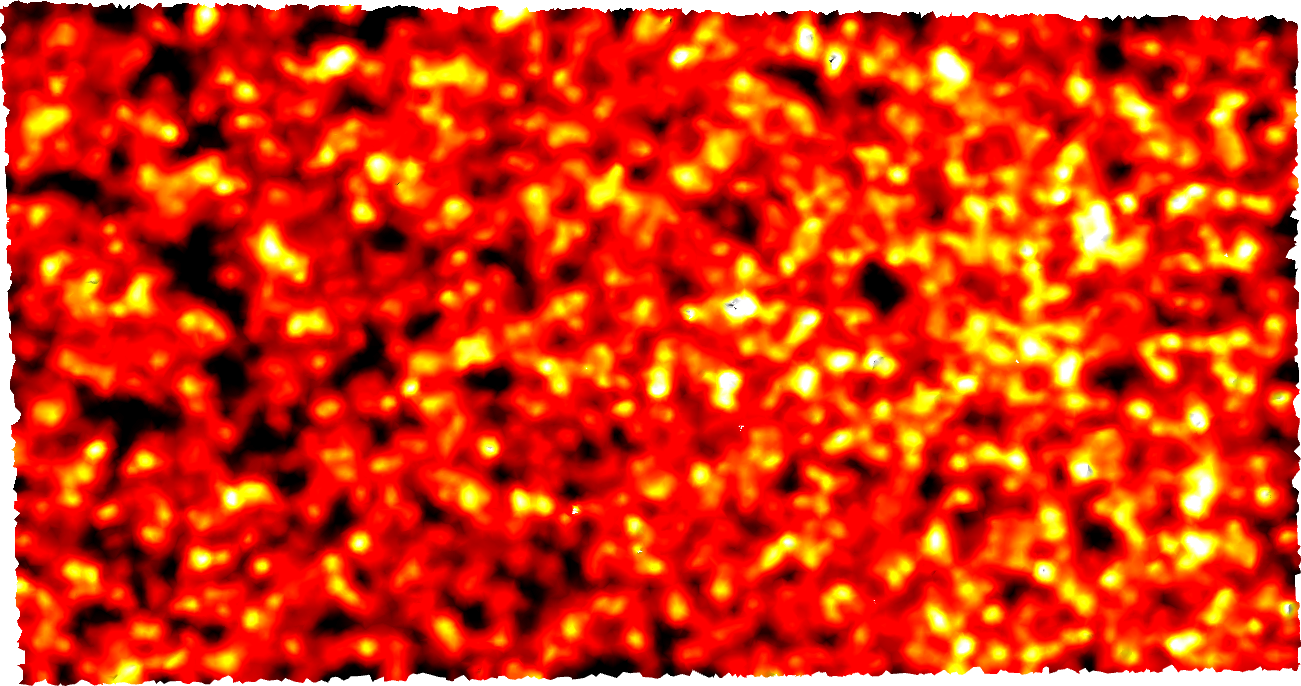
\includegraphics[width=1.0\linewidth,height=0.3\textheight,keepaspectratio]{data/acquired_meshes/ILATO_1A_SM2066-HE5-60_070214_merged_GMO_r1_n4_v256_funcvals_1000iter.png}
		\caption{ILATO 1000iter}\label{fig:ILATO.c}
	\end{subfigure}
	\begin{subfigure}[b]{0.48\linewidth}
		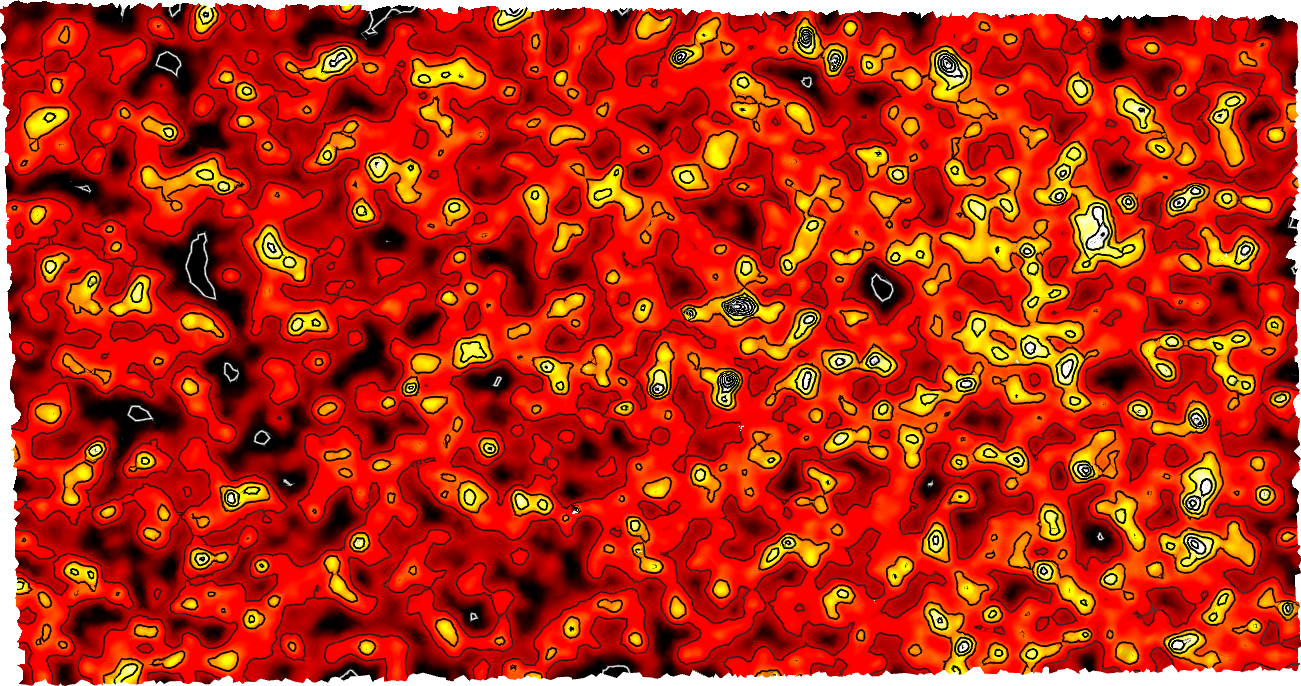
\includegraphics[width=1.0\linewidth,height=0.3\textheight,keepaspectratio]{data/acquired_meshes/ILATO_1A_SM2066-HE5-60_070214_merged_GMO_r1_n4_v256_funcvals_isolines_1000iter.png}
		\caption{ILATO 1000iter isolines}\label{fig:ILATO.d}
	\end{subfigure}

	\bigskip
	\begin{subfigure}[b]{0.48\linewidth}
		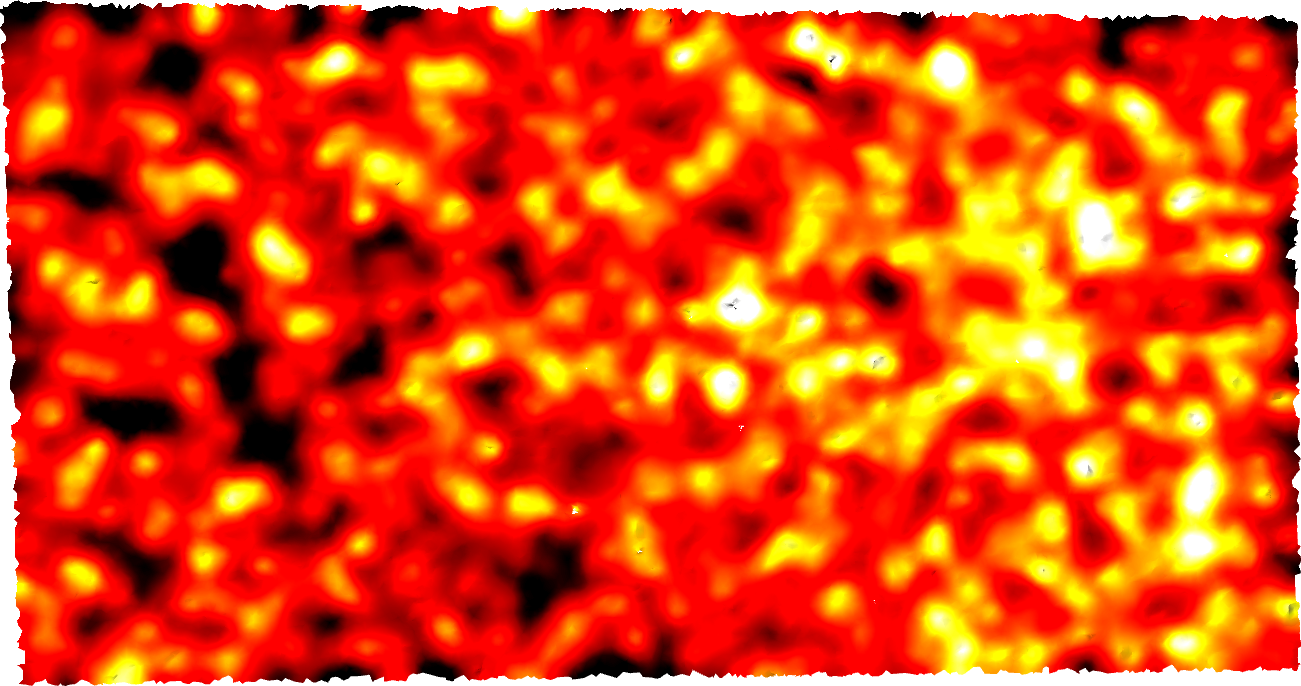
\includegraphics[width=1.0\linewidth,height=0.3\textheight,keepaspectratio]{data/acquired_meshes/ILATO_1A_SM2066-HE5-60_070214_merged_GMO_r1_n4_v256_funcvals_3000iter.png}
		\caption{ILATO 3000iter}\label{fig:ILATO.e}
	\end{subfigure}
	\begin{subfigure}[b]{0.48\linewidth}
		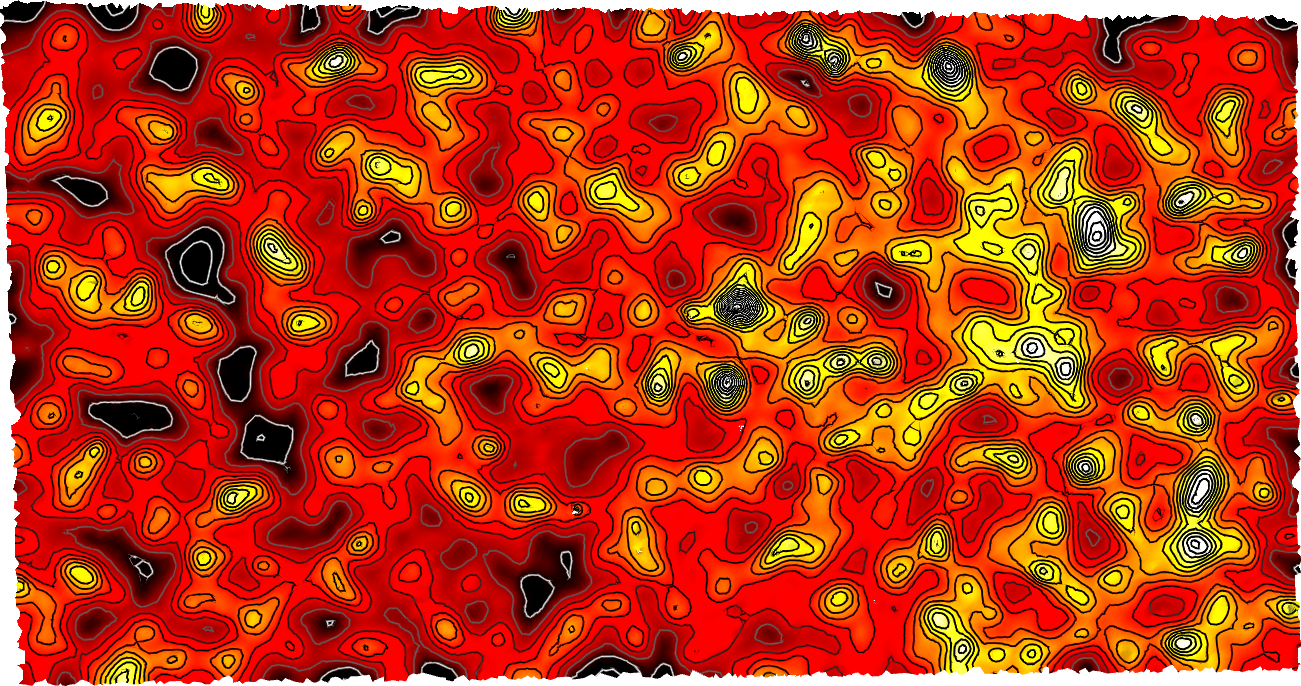
\includegraphics[width=1.0\linewidth,height=0.3\textheight,keepaspectratio]{data/acquired_meshes/ILATO_1A_SM2066-HE5-60_070214_merged_GMO_r1_n4_v256_funcvals_isolines_3000iter.png}
		\caption{ILATO 3000iter isolines}\label{fig:ILATO.f}
	\end{subfigure}}
	{\caption[ILATO]{ILATO\_1A\ldots}\label{fig:ILATO}}
\end{figure}

\subsection{Stanford Bunny}
Figure~\ref{fig:bun}: http://graphics.stanford.edu/data/3Dscanrep/ (Stanford Bunny)
\begin{figure}[ht]
\ffigbox
	{\begin{subfigure}[b]{0.48\linewidth}
		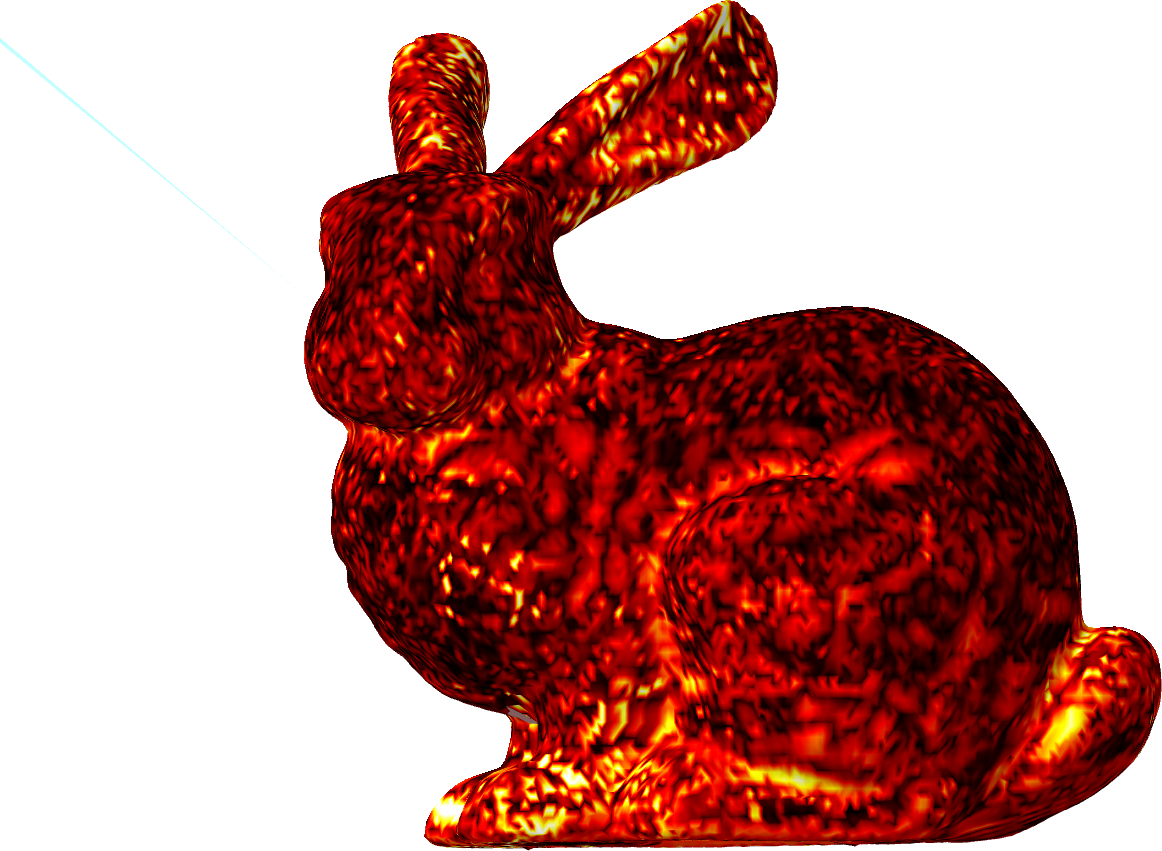
\includegraphics[width=1.0\linewidth,height=0.3\textheight,keepaspectratio]{data/acquired_meshes/bun_zipper_edited_r1_n4_v256_funcvals_0iter.png}
		\caption{Stanford Bunny 0iter}\label{fig:bun.a}
	\end{subfigure}
	\begin{subfigure}[b]{0.48\linewidth}
		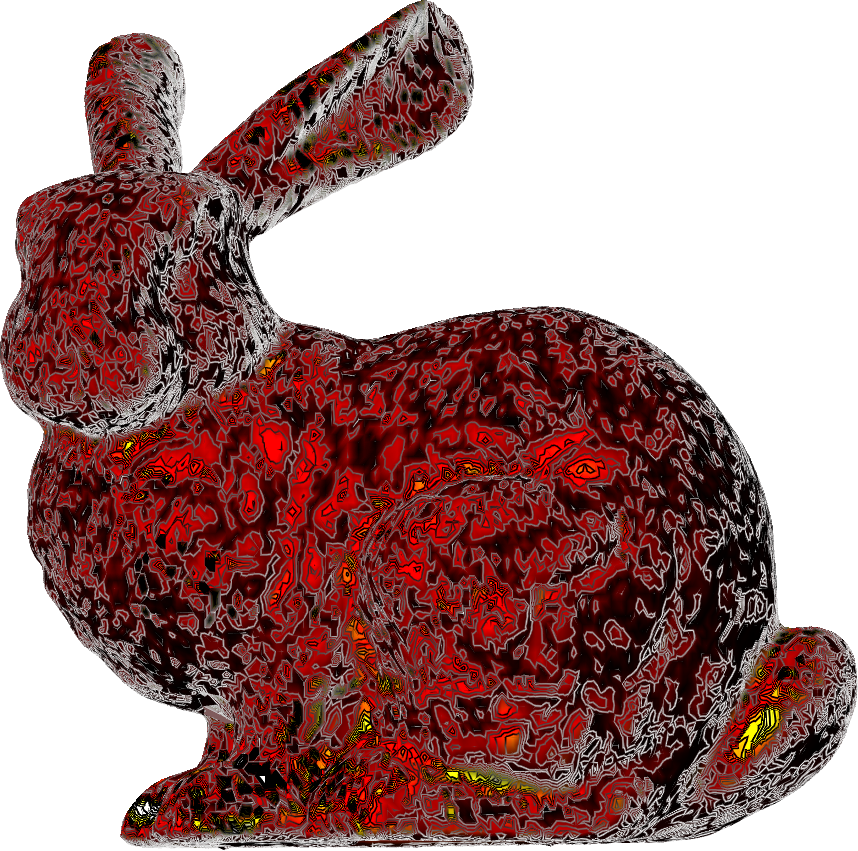
\includegraphics[width=1.0\linewidth,height=0.3\textheight,keepaspectratio]{data/acquired_meshes/bun_zipper_edited_r1_n4_v256_funcvals_isolines_0iter.png}
		\caption{Stanford Bunny 0iter isolines}\label{fig:bun.b}
	\end{subfigure}

	\bigskip
	\begin{subfigure}[b]{0.48\linewidth}
		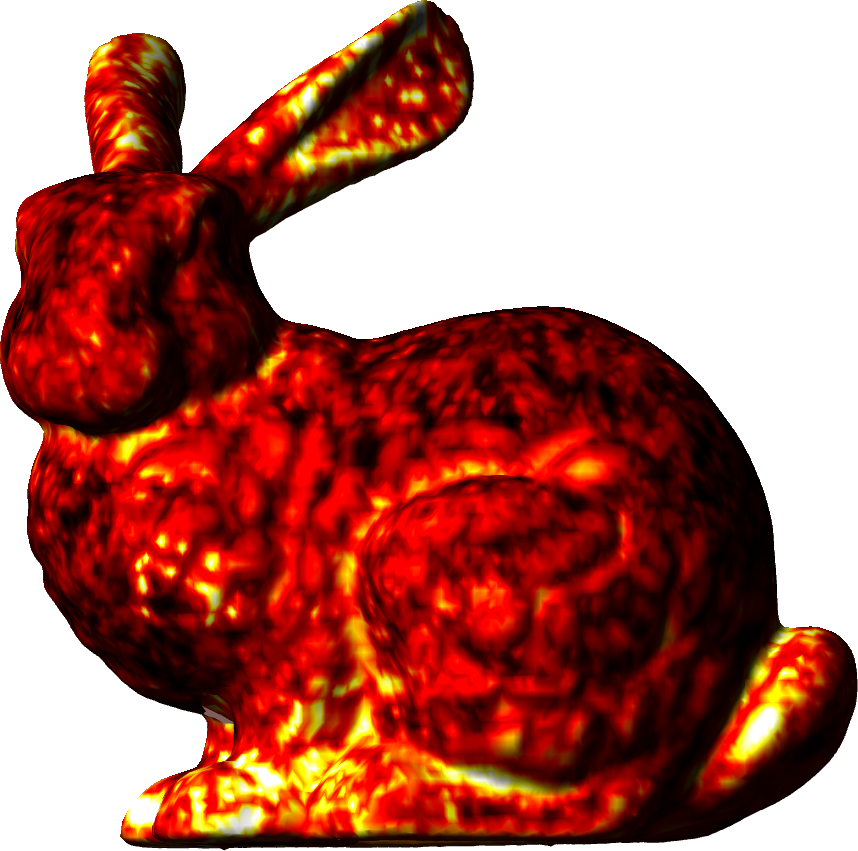
\includegraphics[width=1.0\linewidth,height=0.3\textheight,keepaspectratio]{data/acquired_meshes/bun_zipper_edited_r1_n4_v256_funcvals_10iter.png}
		\caption{Stanford Bunny 10iter}\label{fig:bun.c}
	\end{subfigure}
	\begin{subfigure}[b]{0.48\linewidth}
		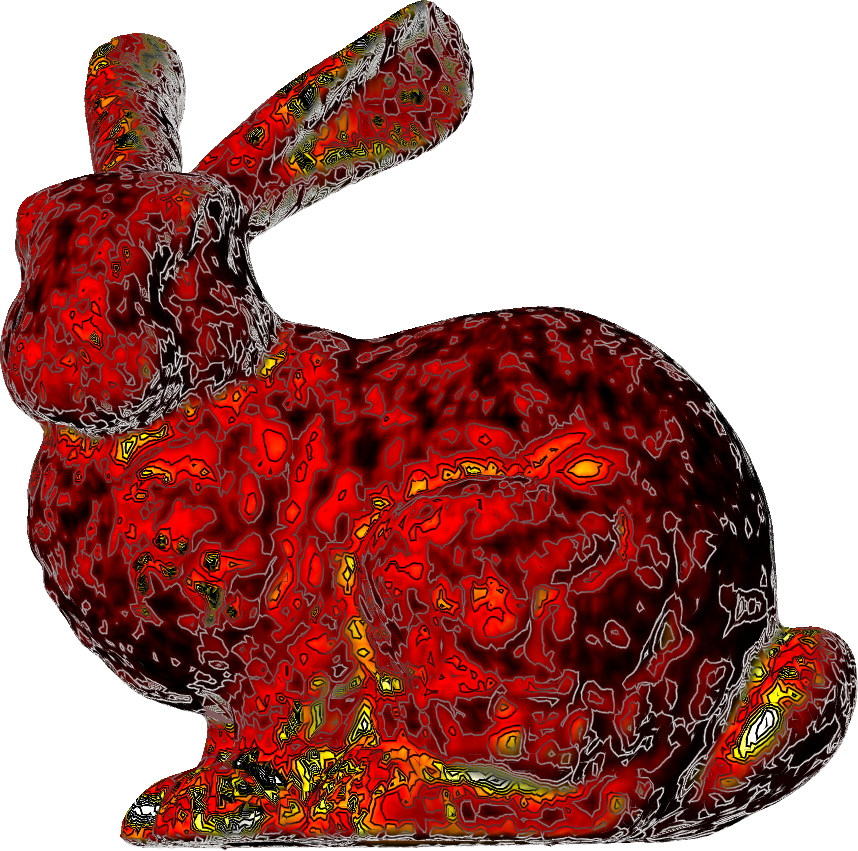
\includegraphics[width=1.0\linewidth,height=0.3\textheight,keepaspectratio]{data/acquired_meshes/bun_zipper_edited_r1_n4_v256_funcvals_isolines_10iter.png}
		\caption{Stanford Bunny 10iter isolines}\label{fig:bun.d}
	\end{subfigure}

	\bigskip
	\begin{subfigure}[b]{0.48\linewidth}
		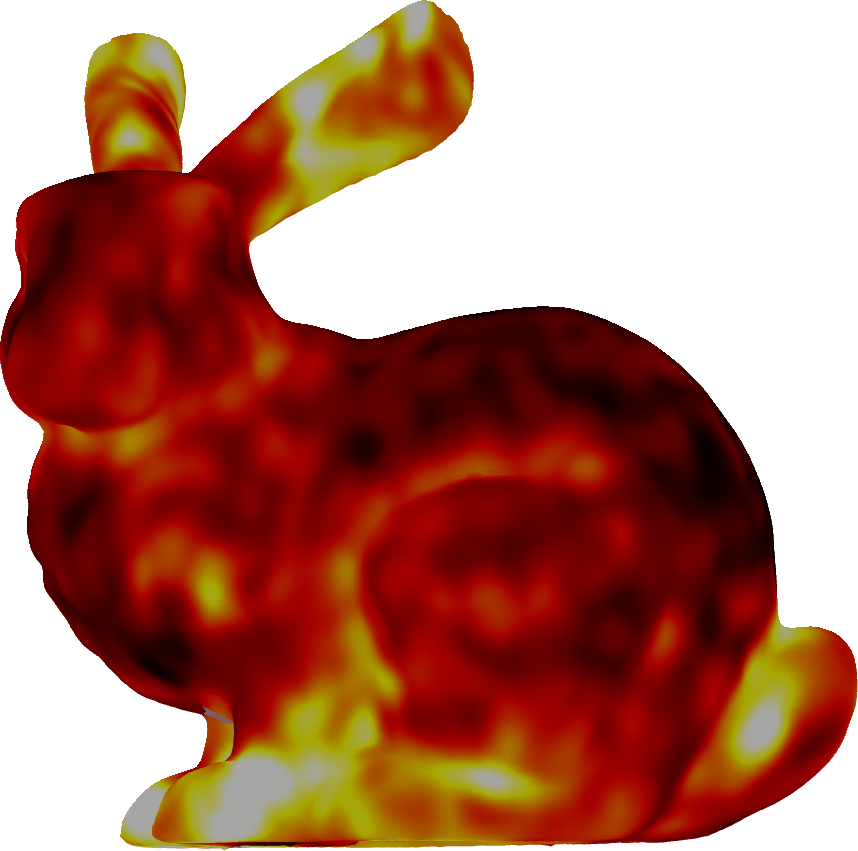
\includegraphics[width=1.0\linewidth,height=0.3\textheight,keepaspectratio]{data/acquired_meshes/bun_zipper_edited_r1_n4_v256_funcvals_100iter.png}
		\caption{Stanford Bunny Wireframe}\label{fig:bun.e}
	\end{subfigure}
	\begin{subfigure}[b]{0.48\linewidth}
		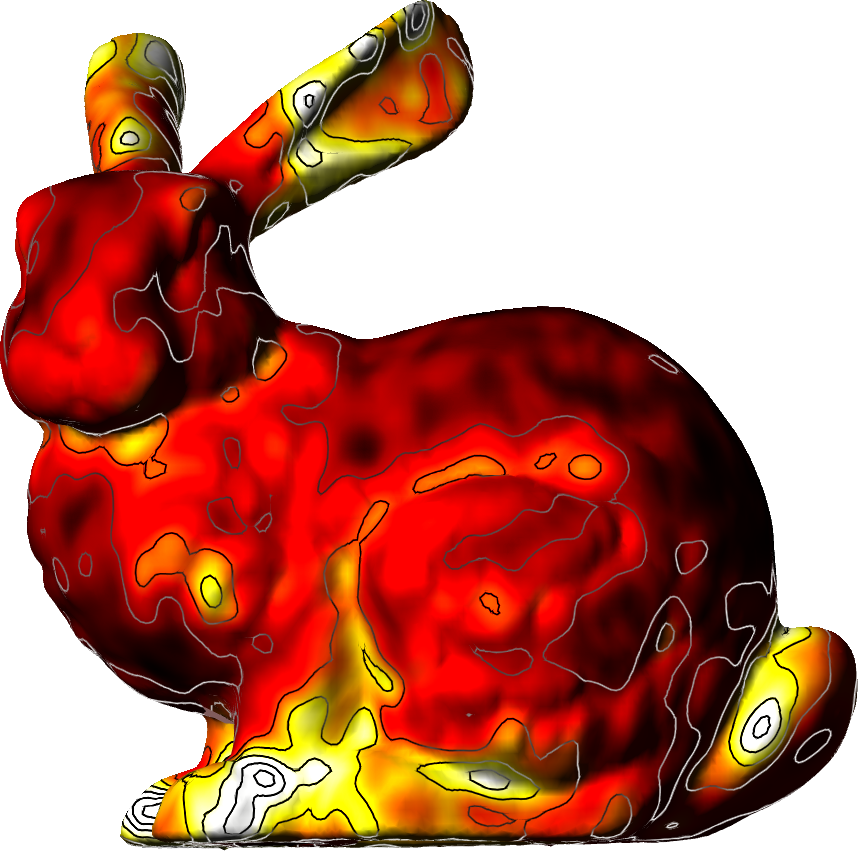
\includegraphics[width=1.0\linewidth,height=0.3\textheight,keepaspectratio]{data/acquired_meshes/bun_zipper_edited_r1_n4_v256_funcvals_isolines_100iter.png}
		\caption{Stanford Bunny 100iter isolines}\label{fig:bun.f}
	\end{subfigure}}
	{\caption[Stanford Bunny]{Stanford Bunny\ldots}\label{fig:bun}}
\end{figure}



\section{Evaluation}
\subsection{Compute Times}

Figure~\ref{fig:computeTimesLP} shows how compute times increase linearly with both mesh size and number of iterations in a very predictable way when total compute time is at least 0.1 seconds, and less predictable for shorter periods do to the nature of thread optimization at the processor level and variable memory read times.\todoResearch{add formula for timing (or at least ref to it) here.}\todoResearch{process time noise at very fast speeds}
\begin{figure}[ht]
	\centering
	\includegraphics[width=1.0\linewidth,height=1.0\textheight,keepaspectratio]{figures/computeTimesLinespoints.png}
	\RawCaption{\caption[Compute Times - Linespoints]{Compute Times of Applying
		the	One-Ring Filter for Selected Numbers of Iterations onto Acquired and
		Synthetic 3D Meshes of Varying Sizes}
		\label{fig:computeTimesLP}}
\end{figure}

Figure~\ref{fig:computeTimesS} shows how compute times increase with both meshsize and number of iterations.\todoCitation{wikipedia Euler characteristic Polyhedra}
\begin{figure}[ht]
	\centering
	\includegraphics[width=1.0\linewidth,height=1.0\textheight,keepaspectratio]{figures/computeTimesScatter.png}
	\RawCaption{\caption[Compute Times - Scatter]{Compute Times for Different
		Hardware Configurations by increaseing Mesh Size and Filter Iterations}
		\label{fig:computeTimesS}}
\end{figure}

\begin{figure}[ht]
	\centering
	\includegraphics[width=1.0\linewidth,height=1.0\textheight,keepaspectratio]{figures/numFacesByVerticesGoTo2.png}
	\RawCaption{\caption[Ratio of Faces / Vertices]{Ratio of Faces to Vertices by
		Increasing Vertex Count}
		\label{fig:ratioFacesVertices}}
\end{figure}





\section{Summary}
Lorem ipsum dolor sit amet, consectetur adipiscing elit. Morbi tincidunt eget
ipsum eu iaculis. Cras vel sem eu velit eleifend porta vel sit amet massa. Etiam
a posuere nunc. Aenean aliquam viverra dapibus. Aliquam ac eros a purus feugiat
rhoncus. Donec faucibus ut nibh ut cursus. Aliquam erat volutpat. Proin efficitur
nulla sit amet iaculis condimentum. Cras placerat leo vitae venenatis feugiat. In
hac habitasse platea dictumst. Orci varius natoque penatibus et magnis dis
parturient montes, nascetur ridiculus mus. In aliquet sagittis dui eu pulvinar.
Morbi a arcu eu dolor sagittis varius. Aliquam dignissim tortor sed tortor
suscipit, eget imperdiet mauris convallis.

\chapter{Distribution}
CLI - commandline interface only
Focus on theoretical work 
And specifics regarding CUDA considerations regarding its limitations
MAYBE 1 page
Dependencies
Linux vs Windows



\section{Standalone Precompiled Binary}
CLI - commandline interface only



\section{Integration with Legacy Code (GigaMesh)}
CLI - commandline interface or GUI - graphical user interface are possible
\begin{enumerate}
\item Make GigaMesh CUDA aware
	\begin{enumerate}
	\item Update Makefile to include nvcc compiler and new source files
	\item second item
	\end{enumerate}
\item second item
\end{enumerate}
Before CUDA 5.0, if a programmer wanted to call particle::advance() from a CUDA 
kernel launched in main.cpp, the compiler required the main.cpp compilation unit 
to include the implementation of particle::advance() as well any subroutines it 
calls (v3::normalize() and v3::scramble() in this case). In complex C++ 
applications, the call chain may go deeper than the two-levels that our example 
illustrates. Without device object linking, the developer may need to deviate 
from the conventional application structure to accommodate this compiler 
requirement. Such changes are difficult for existing applications in which 
changing the structure is invasive and/or undesirable.~\cite{Cuda14}
In order to use the full functionality of GigaMesh a batch program has to be run 
for generating feature vectors. These vectors contain additional information per 
vertex concerning surface and volume of a set of spheres intersecting the mesh. 
See [MKJB10] for more background information on the Multi Scale Integral 
Invariant (MSII) filtering technique. This operation is rather time consuming 
(it takes hours or even days of computing time) and therefore better runs 
without graphical user interface. Although generating feature vectors is quite 
robust against solo vertices, singularities, non-manifolds and holes, you should 
first clean up your mesh data to get a proper result. So switch to the advanced 
task of polishing your mesh in section 4.1 and return to this section when you 
have got a cleaned mesh. If you do not want to manipulate your mesh you may 
continue directly. Open a terminal and type and change to the mesh-folder by 
typing cd GigaMesh/mesh (note that GigaMesh stands for the GigaMesh installation 
folder). Then start the program nohup ./meshgeneratorfeaturevectors25d\_threads 
-f [-r 2] \& and use nohup at the beginning of the command and \& at the end to 
ensure that the job runs in the background. This is because this step can take 
several hours and you do not want to block the terminal.~\cite[p.~19]{Giga17}



\section{Summary}
Lorem ipsum dolor sit amet, consectetur adipiscing elit. Morbi tincidunt eget 
ipsum eu iaculis. Cras vel sem eu velit eleifend porta vel sit amet massa. Etiam 
a posuere nunc. Aenean aliquam viverra dapibus. Aliquam ac eros a purus feugiat 
rhoncus. Donec faucibus ut nibh ut cursus. Aliquam erat volutpat. Proin efficitur 
nulla sit amet iaculis condimentum. Cras placerat leo vitae venenatis feugiat. In 
hac habitasse platea dictumst. Orci varius natoque penatibus et magnis dis 
parturient montes, nascetur ridiculus mus. In aliquet sagittis dui eu pulvinar. 
Morbi a arcu eu dolor sagittis varius. Aliquam dignissim tortor sed tortor 
suscipit, eget imperdiet mauris convallis.

\chapter{Conclusions}
\section{Summary}
Lorem ipsum dolor sit amet, consectetur adipiscing elit. Morbi tincidunt eget 
ipsum eu iaculis. Cras vel sem eu velit eleifend porta vel sit amet massa. Etiam 
a posuere nunc. Aenean aliquam viverra dapibus. Aliquam ac eros a purus feugiat 
rhoncus. Donec faucibus ut nibh ut cursus. Aliquam erat volutpat. Proin efficitur 
nulla sit amet iaculis condimentum. Cras placerat leo vitae venenatis feugiat. In 
hac habitasse platea dictumst. Orci varius natoque penatibus et magnis dis 
parturient montes, nascetur ridiculus mus. In aliquet sagittis dui eu pulvinar. 
Morbi a arcu eu dolor sagittis varius. Aliquam dignissim tortor sed tortor 
suscipit, eget imperdiet mauris convallis.

Aliquam in justo ut est eleifend facilisis vitae nec mi. Suspendisse pellentesque, 
ligula ut mattis volutpat, ex risus scelerisque ligula, at ornare arcu augue ut r
isus. Integer non pellentesque quam, quis laoreet nisi. Donec aliquam leo mi, vel 
consectetur magna vestibulum eu. Ut quis efficitur metus. Donec consequat mi nec 
pellentesque rhoncus. Phasellus sit amet laoreet quam. Quisque dictum ex non elit 
aliquet lobortis. Quisque molestie egestas dolor vel interdum. In fermentum sit 
amet mi non venenatis. In ut tempus arcu.

Donec arcu eros, vestibulum maximus volutpat nec, euismod a purus. Nullam bibendum 
eros posuere sem sollicitudin, vitae porttitor ex scelerisque. Sed nisi felis, 
consectetur sed lacinia vitae, egestas non nibh. Curabitur a ex sed neque lacinia 
tempor sit amet consectetur ipsum. Sed et eros dictum, dictum magna lacinia, 
elementum lacus. Praesent enim tortor, semper ut egestas at, faucibus quis metus. 
Aliquam mattis, lorem et ultrices mattis, erat neque bibendum est, nec condimentum 
ex tellus sit amet diam. In sollicitudin placerat diam, lobortis efficitur leo. 
Integer id erat tellus. Ut quis odio velit. Nulla facilisi. Donec mollis 
scelerisque lobortis. Nam eu felis sed purus feugiat semper ac ac ante. Maecenas 
faucibus odio diam, id tristique orci placerat sed. Ut vel ex metus. Maecenas 
tempus velit gravida nulla viverra, in suscipit enim mattis.


\section{Future Work}
What they are and why I did not.
OpenMP
PThreads
(already impl’d in GigaMesh)
OpenCL
Pipelining memory reads/calculations exploit more concurrency
Thread indexing 3D vs 1D
Determine is using $\Dm$ vs $\bar{\Dm}$ has any effect, especially on one-ring neighborhood with a relatively large $\Dm$ on mesh with a very small $\bar{\Dm}$ 

%
\appendix
\chapter{Maybe some appendix please?}
Lorem ipsum dolor sit amet, consectetur adipiscing elit. Morbi tincidunt eget 
ipsum eu iaculis. Cras vel sem eu velit eleifend porta vel sit amet massa. Etiam 
a posuere nunc. Aenean aliquam viverra dapibus. Aliquam ac eros a purus feugiat 
rhoncus. Donec faucibus ut nibh ut cursus. Aliquam erat volutpat. Proin efficitur 
nulla sit amet iaculis condimentum. Cras placerat leo vitae venenatis feugiat. In 
hac habitasse platea dictumst. Orci varius natoque penatibus et magnis dis 
parturient montes, nascetur ridiculus mus. In aliquet sagittis dui eu pulvinar. 
Morbi a arcu eu dolor sagittis varius. Aliquam dignissim tortor sed tortor 
suscipit, eget imperdiet mauris convallis.

Aliquam in justo ut est eleifend facilisis vitae nec mi. Suspendisse pellentesque, 
ligula ut mattis volutpat, ex risus scelerisque ligula, at ornare arcu augue ut r
isus. Integer non pellentesque quam, quis laoreet nisi. Donec aliquam leo mi, vel 
consectetur magna vestibulum eu. Ut quis efficitur metus. Donec consequat mi nec 
pellentesque rhoncus. Phasellus sit amet laoreet quam. Quisque dictum ex non elit 
aliquet lobortis. Quisque molestie egestas dolor vel interdum. In fermentum sit 
amet mi non venenatis. In ut tempus arcu.

Donec arcu eros, vestibulum maximus volutpat nec, euismod a purus. Nullam bibendum 
eros posuere sem sollicitudin, vitae porttitor ex scelerisque. Sed nisi felis, 
consectetur sed lacinia vitae, egestas non nibh. Curabitur a ex sed neque lacinia 
tempor sit amet consectetur ipsum. Sed et eros dictum, dictum magna lacinia, 
elementum lacus. Praesent enim tortor, semper ut egestas at, faucibus quis metus. 
Aliquam mattis, lorem et ultrices mattis, erat neque bibendum est, nec condimentum 
ex tellus sit amet diam. In sollicitudin placerat diam, lobortis efficitur leo. 
Integer id erat tellus. Ut quis odio velit. Nulla facilisi. Donec mollis 
scelerisque lobortis. Nam eu felis sed purus feugiat semper ac ac ante. Maecenas 
faucibus odio diam, id tristique orci placerat sed. Ut vel ex metus. Maecenas 
tempus velit gravida nulla viverra, in suscipit enim mattis.

\chapter{Just another appendix.}
Lorem ipsum dolor sit amet, consectetur adipiscing elit. Morbi tincidunt eget 
ipsum eu iaculis. Cras vel sem eu velit eleifend porta vel sit amet massa. Etiam 
a posuere nunc. Aenean aliquam viverra dapibus. Aliquam ac eros a purus feugiat 
rhoncus. Donec faucibus ut nibh ut cursus. Aliquam erat volutpat. Proin efficitur 
nulla sit amet iaculis condimentum. Cras placerat leo vitae venenatis feugiat. In 
hac habitasse platea dictumst. Orci varius natoque penatibus et magnis dis 
parturient montes, nascetur ridiculus mus. In aliquet sagittis dui eu pulvinar. 
Morbi a arcu eu dolor sagittis varius. Aliquam dignissim tortor sed tortor 
suscipit, eget imperdiet mauris convallis.

Aliquam in justo ut est eleifend facilisis vitae nec mi. Suspendisse pellentesque, 
ligula ut mattis volutpat, ex risus scelerisque ligula, at ornare arcu augue ut r
isus. Integer non pellentesque quam, quis laoreet nisi. Donec aliquam leo mi, vel 
consectetur magna vestibulum eu. Ut quis efficitur metus. Donec consequat mi nec 
pellentesque rhoncus. Phasellus sit amet laoreet quam. Quisque dictum ex non elit 
aliquet lobortis. Quisque molestie egestas dolor vel interdum. In fermentum sit 
amet mi non venenatis. In ut tempus arcu.

Donec arcu eros, vestibulum maximus volutpat nec, euismod a purus. Nullam bibendum 
eros posuere sem sollicitudin, vitae porttitor ex scelerisque. Sed nisi felis, 
consectetur sed lacinia vitae, egestas non nibh. Curabitur a ex sed neque lacinia 
tempor sit amet consectetur ipsum. Sed et eros dictum, dictum magna lacinia, 
elementum lacus. Praesent enim tortor, semper ut egestas at, faucibus quis metus. 
Aliquam mattis, lorem et ultrices mattis, erat neque bibendum est, nec condimentum 
ex tellus sit amet diam. In sollicitudin placerat diam, lobortis efficitur leo. 
Integer id erat tellus. Ut quis odio velit. Nulla facilisi. Donec mollis 
scelerisque lobortis. Nam eu felis sed purus feugiat semper ac ac ante. Maecenas 
faucibus odio diam, id tristique orci placerat sed. Ut vel ex metus. Maecenas 
tempus velit gravida nulla viverra, in suscipit enim mattis.

%
\backmatter
\printindex
\bibliography{thesis}{}
\bibliographystyle{plain}
\todoRemove{remove todoCitation from bibliography}
\todoStyle{should bibliographystyle be plain?}

\end{document}

